\special{pdf:minorversion 7}
\PassOptionsToPackage{dvipsnames}{xcolor}
\documentclass[12pt,letterpaper,twoside]{report}

\usepackage[todonotes={textsize=scriptsize}, final]{changes}
\usepackage[left=1in, right=1in, top=1in, bottom=1in]{geometry}
\usepackage{setspace}
\usepackage{layout}
\usepackage{parskip}
\usepackage{amsmath}
\usepackage{amssymb}
\usepackage[T1]{fontenc}
\usepackage{fontspec}
\setmainfont{XCharter}
\usepackage{unicode-math}
\setmathfont{XCharter-Math.otf}
\setsansfont{IBMPlexSans}[
    Extension = .otf,
    UprightFont = *-Regular,
    BoldFont = *-SemiBold,
    ItalicFont = *-Italic,
    BoldItalicFont = *-SemiBoldItalic,
    Scale = MatchLowercase
]
\setmonofont{IBMPlexMono}[Scale=MatchLowercase]
\usepackage{multicol}
\usepackage{multirow}
\usepackage{pdfpages}
\usepackage{pdflscape}
\usepackage{afterpage}
\usepackage{graphicx}
% \DeclareGraphicsExtensions{.png,.pdf}
\DeclareGraphicsExtensions{.pdf,.png}
\usepackage{tabularx}
% \usepackage{expl3}
% \usepackage{calc}
\usepackage[version=4]{mhchem}
\usepackage{siunitx}
\usepackage{bm}
\usepackage[dvipsnames]{xcolor}
\usepackage{caption}
\usepackage{subcaption}
\usepackage[sf,bf]{titlesec}
\usepackage{colortbl}
\usepackage{enumitem}
\usepackage{listings}
\usepackage{booktabs}
\usepackage{gensymb}
\usepackage[font=itshape]{quoting}
\usepackage{wrapfig}
\usepackage{fancyhdr}
\usepackage{lipsum}
\usepackage[final]{draftwatermark}
\usepackage{soul}
\usepackage[
    style=ieee,
    citestyle=numeric-comp,
    urldate=iso]{biblatex}
% \usepackage{datetime}
\usepackage{nameref}
\usepackage{hyperref}
\usepackage{tablefootnote}
\usepackage{todonotes}
\onehalfspacing
\definecolor{McGillRed}{cmyk}{0, 1, 0.9, 0}
\hypersetup{
    colorlinks=true,
    linkcolor=cyan,
    anchorcolor=cyan,
    citecolor=cyan,
    filecolor=cyan,
    urlcolor=cyan
}
\setdeletedmarkup{\textcolor{McGillRed}{\sout{#1}}}
% \setdeletedmarkup{\textcolor{McGillRed}{#1}}
\definechangesauthor[color=violet, name={Emmanuel Duplay}]{ED}
\definechangesauthor[color=cyan, name={Barry Zandbergen}]{BZ}
\definechangesauthor[color=McGillRed, name={Andrew Higgins}]{AH}

% \input{titlesec.tex}
\addbibresource{ref.bib}

\title{Laser-Powered Rocket Engine: small-scale experimental investigation}
\author{Gabriel Dubé}
\date{0000-00-00}

\renewcommand{\headrulewidth}{0pt}
\renewcommand{\chaptermark}[1]{\markboth{\MakeUppercase{\thechapter.\ #1}}{}}
\renewcommand{\sectionmark}[1]{\markright{\MakeUppercase{\thesection.\ #1}}}

\renewcommand{\chapterautorefname}{Chapter}
\renewcommand{\sectionautorefname}{Section}

\newcommand{\shotsettings}[4]{\texttt{#1}: #2~ms, \textit{f}/#3, ND#4}

\newcommand{\dd}[2]{\frac{\mathrm{d}#1}{\mathrm{d}#2}}
\newcommand{\ddi}[2]{\mathrm{d}#1/\mathrm{d}#2}

\newcommand{\blankpage}{%
    \null
    \thispagestyle{empty}%
    \addtocounter{page}{-1}%
    \newpage}

% Track changes commands
% \newcommand{\change}[1]{\textcolor{McGillRed}{#1}}
% \newenvironment{changeblock}{\color{McGillRed}}{}
% \renewcommand{\change}[1]{#1}  % Comment out to suppress changes
% \renewenvironment{changeblock}{}{}  % Comment out to suppress changes

\fancypagestyle{fancy}{
    \fancyhf{}
    \fancyhfinit{\sffamily}
    \lhead{\leftmark}
    \rhead{\rightmark}
    % \lfoot{AE5050}
    % \rfoot{\thepage}
    \fancyfoot[LE,RO]{\thepage}
    %\fancyfoot[RE,LO]{AE5050}
}

\fancypagestyle{plain}{
    \fancyhf{}
    \fancyfoot[C]{\sffamily \thepage}
    
}

\pagestyle{fancy}

\SetWatermarkText{\sffamily \textbf{DRAFT}}
\SetWatermarkFontSize{2cm}
\SetWatermarkColor[gray]{0.85}
    
\definecolor{bggray}{gray}{0.97}
\definecolor{txtgray}{gray}{0.3}

\lstdefinestyle{mystyle}{
    backgroundcolor=\color{bggray},   
    commentstyle=\color{MidnightBlue},
    keywordstyle=\color{Plum},
    numberstyle=\scriptsize\ttfamily\color{Gray},
    stringstyle=\color{RedOrange},
    % identifierstyle=\color{Turquoise},
    basicstyle=\ttfamily\color{txtgray},
    breakatwhitespace=false,         
    breaklines=true,                 
    captionpos=t,                    
    keepspaces=true,                 
    numbers=left,                    
    numbersep=5pt,                  
    showspaces=false,                
    showstringspaces=false,
    showtabs=false,                  
    tabsize=2
}

\lstset{style=mystyle}
\newenvironment{plainchp}[1]
    {
        \newgeometry{left=4.2cm,right=4.2cm}
        \fancypagestyle{abstractplain}{
            \fancyhf{}
            \fancyfootoffset[lh]{0pt}
            \fancyfoot[C]{\sffamily \thepage}  
        }
        \pagestyle{abstractplain}
        
        \phantomsection
        \begin{center}
            \sffamily \Large \caps{\textbf{\MakeUppercase{#1}}}
        \end{center}
        \vspace{0.2cm}
        \markboth{\MakeUppercase{#1}}{}
    }
    {
        \restoregeometry
        \pagestyle{fancy}
    }

\newenvironment{statement}[1]
    {
        \vspace{\parskip}
        \begin{center}\begin{minipage}{0.85\textwidth}
            {\sffamily \footnotesize \color{cyan}\caps{\MakeUppercase{#1}}}\\\itshape
    }
    {
        \end{minipage}\end{center}
        \vspace{\parskip}
    }

\sisetup{detect-all}

\begin{document}
    \setlength{\parindent}{0pt}
    \setlength{\headheight}{15pt}
    % 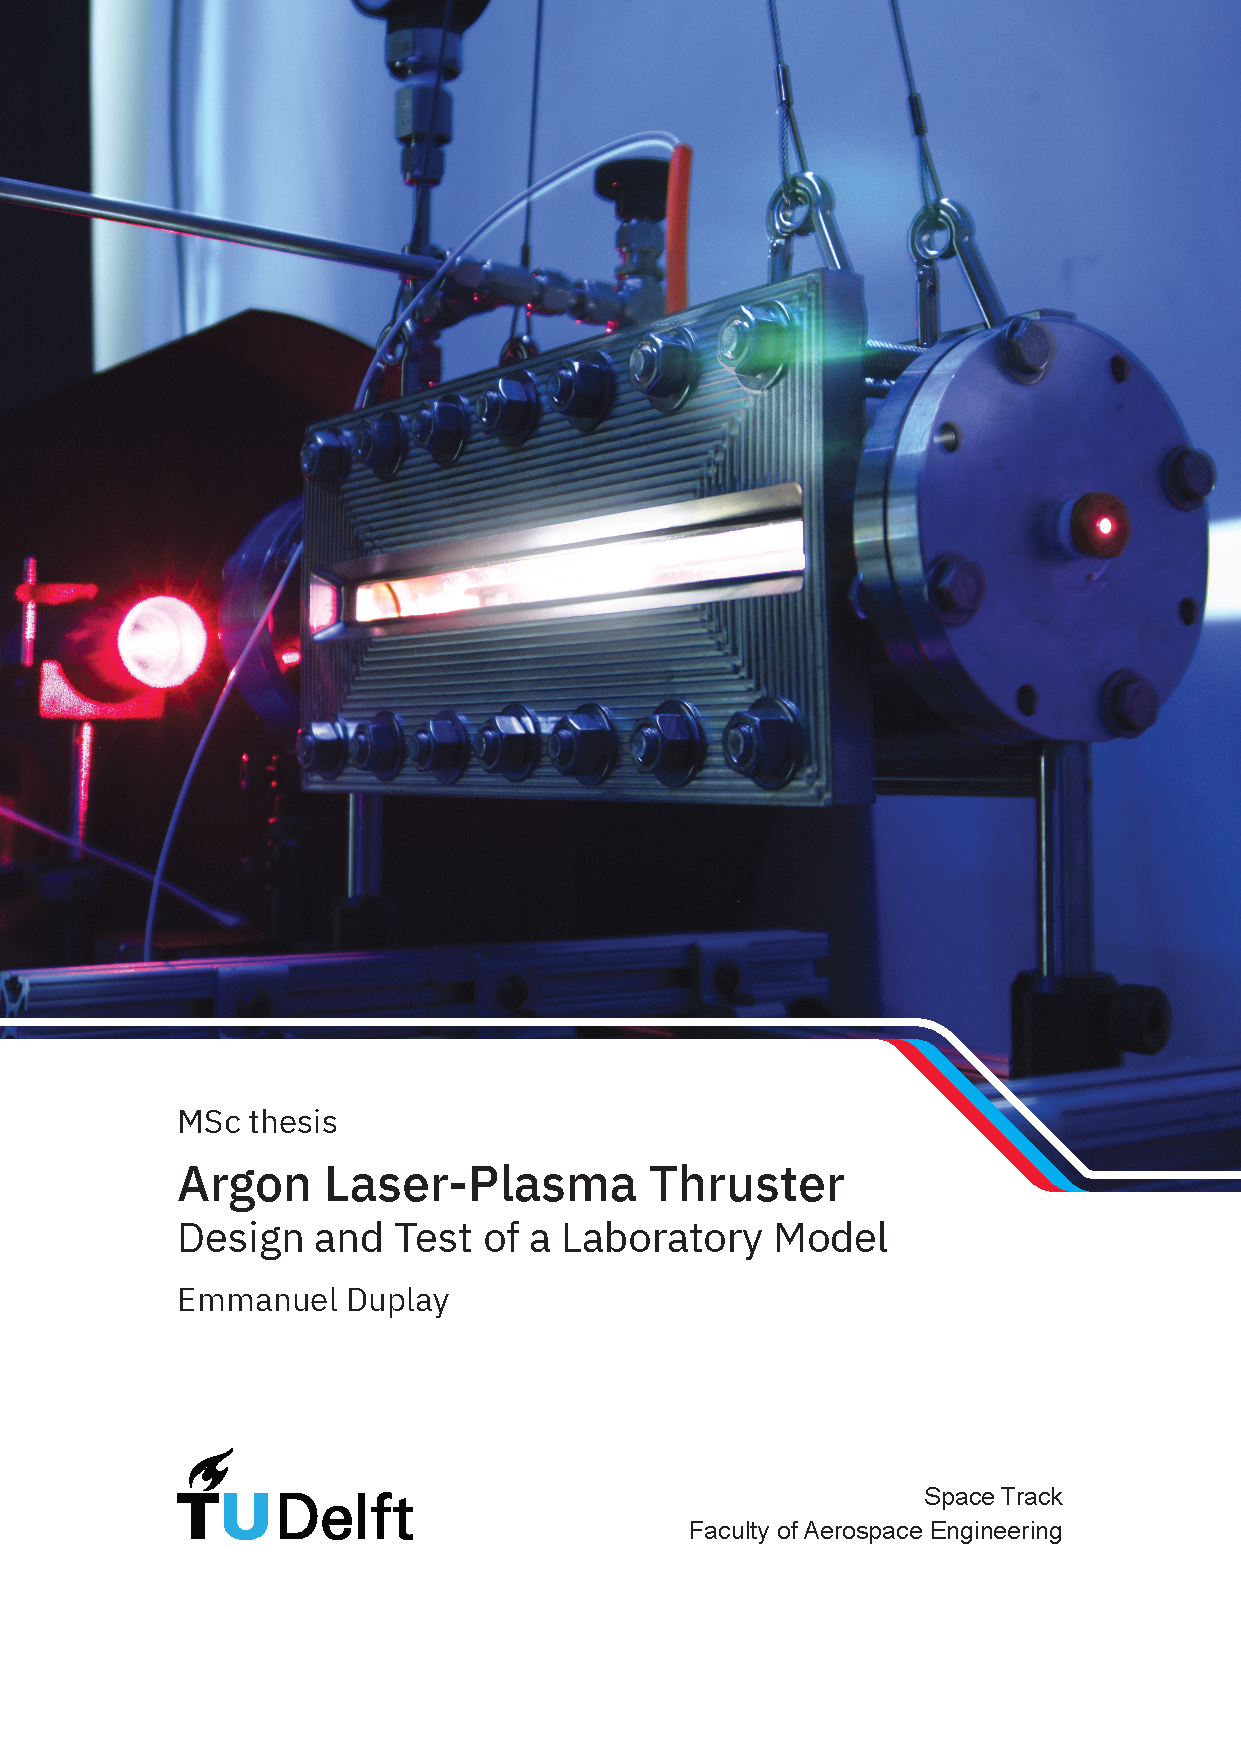
\includepdf{assets/cover.pdf}
    \begin{titlepage}
  \thispagestyle{empty}
  \sffamily
  \begin{center}
    
\includegraphics[width=0.5\textwidth]{assets/McGill_logo.pdf} \\
    \vspace*{2cm}
    
    \huge
    \textbf{Design and validation of an Argon Laser Thermal Propulsion Thruster Powered by a Fiber Laser}
    
    \large
    % \textit{Small-scale experimental investigation}     

    
    \vspace{1.5cm}    
    \textbf{Gabriel Roland Dubé}\\

    
    \vspace{0.5cm}
    Department of Mechanical Engineering\\
    McGill University, Montreal\\

    \vspace{1.5cm}
    April 2025\\
    \vspace{1.5cm}
    
    A thesis submitted to McGill University \\
    in partial fulfillment of the requirements of the degree of\\
    \textbf{Master of Science}\\
    
    %\vskip 10mm
    \vfill

    {\color{red}\hrule}

    \copyright Gabriel Roland Dubé, 2025
            
  \end{center}
\end{titlepage}

    % \newpage
    % % \layout*
    % {   \sffamily
    %     \thispagestyle{empty}
    %     \vspace*{\fill}
    %     % Text width: \the\textwidth  \\ % DELETE THIS LINE BEFORE SUBMITTING
    %     % Text height: \the\textheight  % DELETE THIS LINE BEFORE SUBMITTING

    %     The code used for this project (including the \LaTeX\hspace{0.67ex}source) is available on \\ \url{https://github.com/eeduplay/MScThesis}

    %     The author can be contacted by email at \href{mailto:gdub529@gmail.com}{gdub529@gmail.com}

    %     Cover image: Composite photograph approximating (with some artistic license) the appearance of the second generation laser-thermal thruster model operating in the laboratory.
    % }
    \pagenumbering{roman}
    
    
    \hypersetup{linkcolor=black}
    \tableofcontents
    
    \listoffigures
    \addcontentsline{toc}{chapter}{List of Figures}
    
    \listoftables
    \addcontentsline{toc}{chapter}{List of Tables}
    \hypersetup{linkcolor=cyan}
    
    %\chapter*{Nomenclature}
\setlength{\columnsep}{1cm}
\newenvironment{nomtable}
    {
        \centering
        \tabularx{\columnwidth}{r>{\raggedright\arraybackslash}X}
    }
    {
        \endtabularx
    }
\newenvironment{nomlist}
    {
        \begin{itemize}[leftmargin=1.5cm]
            \raggedright
            \setlength{\parsep}{0pt}
            \setlength{\itemsep}{-4pt}
    }
    {
        \end{itemize}
    }
\addcontentsline{toc}{chapter}{Nomenclature}
\markboth{\MakeUppercase{Nomenclature}}{}
\begin{multicols*}{2}
    % \setlength{\columnseprule}{1pt}
    \section*{Abbreviations}

    \begin{nomlist}
        \item[AEC   ] Atomic Energy Commission
        \item[AIAA  ] American Institute of Aeronautics and Astronautics
        \item[CFD   ] Computational Fluid Dynamics
        \item[CFL   ] Courant--Friedrichs--Lewy
        \item[DE    ] Directed-Energy 
        \item[DOE   ] (US) Department of Energy
        \item[FTCS  ] Forward Time Centered Space
        \item[HET   ] Hall-Effect Thruster
        \item[ITER  ] International Thermonuclear Experimental Reactor
        \item[LEP   ] Laser-Electric Propulsion
        \item[LSC   ] Laser-Supported Combustion
        \item[LSP   ] Laser-Sustained Plasma
        \item[LTP   ] Laser-Thermal Propulsion
        \item[NSTX] National Spherical Torus eXperiment
        \item[OOP] Object-Oriented Programming
        \item[OTV]  Orbital Transfer Vehicle 
        \item[PDE] Partial Differential Equation
        \item[PPPL  ] Princeton Plasma Physics Laboratory
        \item[SOR   ] Successive Over-Relaxation
        \item[TUD   ] Technische Universiteit Delft
    \end{nomlist}

    \section*{Latin symbols}
    \begin{nomlist}
        \item[$C$]             Courant number
        \item[$c_p$]           Specific heat of enthalpy
        \item[$D$]             Diameter
        \item[$d$]             Distance
        \item[$g_0$]           Standard gravity (9.80665~\unit{m/s^2}) 
        \item[$h$          ]   Enthalpy
        \item[$I$          ]   Local laser flux [W/m$^2$]
        \item[$I_\text{sp}$]   Specific impulse [s]
        \item[$k_L$        ]   Radiation absorption factor [1/m]
        \item[$m$]             Mass
        \item[$\mathcal{M}$]   Molar mass
        \item[$p$          ]   Pressure
        \item[$R$]             Gas constant
        \item[$r$          ]   Radial coordinate
        \item[$T$          ]   Temperature
        \item[$t$          ]   Time
        \item[$u$          ]   Axial velocity
        \item[$v$]             Velocity 
        \item[$z$          ]   Axial coordinate
    \end{nomlist}

    \section*{Greek symbols}
    \begin{nomlist}
        \item[$\alpha$]    Ionization mole fraction
        \item[$\beta$]     Dissociation mole fraction
        \item[$\theta$]    Azimuthal coordinate
        \item[$\kappa$]    Conductivity
        \item[$\lambda$]   Wavelength
        \item[$\rho$  ]    Density
        \item[$\phi$  ]    Radiation emission [W/m$^3$]
    \end{nomlist}

    \section*{Subscripts}
    \begin{nomlist}
        \item[c]   Thrust chamber
        \item[e]   Laser emitter
        \item[ex]  Exhaust
        \item[f]   Focusing length
        \item[g]   Specific (gas constant)
        \item[$i$] index along $x$ or $z$
        \item[$j$] index along $y$ or $r$
        \item[r]   Laser receiver
        \item[u]   Universal (gas constant)
    \end{nomlist}

    % \section*{Superscripts}
    % \begin{nomlist}
    %     \item[$n$]  time index
    % \end{nomlist}

\end{multicols*}

    \newpage
    \begin{plainchp}{Executive Summary}
    \addcontentsline{toc}{chapter}{Executive Summary}

    \lipsum[2-5]

\end{plainchp}
    % LTeX: language=fr

\begin{plainchp}{Résumé}
    \addcontentsline{toc}{chapter}{Résumé}

    Pour des missions spatiales ambitieuses comme le transit rapide d'humains vers Mars, les méthodes de propulsion conventionnelles ne sont pas à la hauteur. La propulsion laser-thermique (LTP) utilise des lasers pour chauffer le gaz propulseur, générant ainsi de la poussée avec une impulsion spécifique potentiellement plus grande que les moteurs fusées traditionnels. Deux propulseurs LTP à l'échelle du laboratoire ont été testés dans cette thèse, désignés Version 1 (V1) et Version 2 (V2). Version 1 a permis les essais initiaux et la visualisation de la propagation de l'onde du plasma soutenu par laser (LSP). Un prototype d'un propulseur réel, Version 2 a été optimisé pour les essais de poussée. Le processus de conception du propulseur amélioré V2 est également présenté. Ces deux propulseurs seront alimentés par un laser à fibre de \qty{1.07}{μm} ayant une puissance ondes continues (CW) de \qty{300}{W} et une puissance à ondes quasi continues (QCW) de \qty{3}{kW}. L'argon a été utilisé comme gaz propulseur à une pression de \qty{20}{bar}, sélectionné pour sa facilité d'ionisation. Utilisant une bobine de type automobile, l'amorçage par étincelle du LSP QCW a été implémenté avec succès dans V1 et V2. L'ensemencement de l'argon avec du dioxyde d'azote (\ce{NO2}) à des pressions partielles comprises entre \qtyrange{.12}{.55}{bar} a montré que le gaz absorbait plus du double de l'énergie laser par rapport au propergol d'argon pur. Pour augmenter le flux laser vers le plasma, un système optique composé de deux lentilles a été conçu. Différentes lentilles ont été comparées à l'aide d'un logiciel de traçage de rayons (WinLens3D). Un LSP CW a été obtenu avec V2, d'une durée de \qty{85.1}{ms}. Cela représente une durée de vie 1.7 fois plus longue que la longueur d'impulsion QCW maximale de \qty{50.0}{ms} à cette puissance. La poussée moyenne à froid de V2 était de \qty{0.96}{N}. Afin d'interpréter les résultats expérimentaux, un modèle de transfert de chaleur zéro dimension (0D) a été écrit en Python, en utilisant le Bremsstrahlung comme mécanisme de radiation. Enfin, des pistes d'amélioration du propulseur V2 et du support de poussée sont présentées pour permettre à terme un essai de poussée à chaud CW.
    
\end{plainchp}
    % \newgeometry{left=4.2cm,right=4.2cm}
% \fancypagestyle{abstractplain}{
%     \fancyhf{}
%     \fancyfootoffset[lh]{0pt}
%     \fancyfoot[C]{\sffamily \thepage}  
% }
% \pagestyle{abstractplain}

% \phantomsection
% \begin{center}
%     \sffamily \Large \textbf{\caps{PREFACE}}
% \end{center}
%     \addcontentsline{toc}{chapter}{Preface}
%     \markboth{\MakeUppercase{Preface}}{}
%     \label{chp:preface}
%     \vspace{0.2cm}
%     This report documents the work done during my three month internship at the Princeton Plasma Physics Laboratory (PPPL). This project stems from a collaboration between McGill University and the PPPL, following the publication of \citetitle*{duplay_design_2022}, a mission design paper I worked on while finishing my undergraduate studies at McGill. This opportunity to collaborate arose about a month before the start of the summer, as I was still struggling to find an internship, so I would like to thank my former supervisor Andrew Higgins for arranging this experience. I would also like to thank Zhuofan Bao and Paria Makaremi-Esfarjani for their assistance with parts of this project. Finally, thanks to Ahmed Diallo, my supervisor at the PPPL, for inviting me to the PPPL and being a wonderful host.

% \restoregeometry
% \pagestyle{fancy}

\begin{plainchp}{Preface}
    \addcontentsline{toc}{chapter}{Preface}
    This report documents the work done during my three month internship at the Princeton Plasma Physics Laboratory (PPPL). This project stems from a collaboration between McGill University and the PPPL, following the publication of \citetitle*{duplay_design_2022}, a mission design paper I worked on while finishing my undergraduate studies at McGill. This opportunity to collaborate arose about a month before the start of the summer, as I was still struggling to find an internship, so I would like to thank my former supervisor Andrew Higgins for arranging this experience. I would also like to thank Zhuofan Bao and Paria Makaremi-Esfarjani for their assistance with parts of this project. Finally, thanks to Ahmed Diallo, my supervisor at the PPPL, for inviting me to the PPPL and being a wonderful host.
\end{plainchp}
    \afterpage{\blankpage}
    \newpage
    \pagenumbering{arabic}

    % \chapter*{Unnumbered Chapter}
% \addcontentsline{toc}{chapter}{Unnumbered Chapter}  % Uncomment to include in ToC
% \markboth{\MakeUppercase{Unnumbered Chapter}}{} 
    %UNCOMMENT THESE!!!!
    \chapter{Introduction} \label{chp:intro}
    
    \section{Motivation}

        In 2016, the Breakthrough Starshot initiative was proposed based on the work of \textcite{lubinRoadmapInterstellarFlight2016}. This mission involves sending \qty{1}{g} space probes to Alpha Centauri at \qty{20}{\%} the speed of light, using massive ground-based laser arrays. This could be enabled by a Moore's law in fiber laser technology, with a rapid doubling of power and a similar exponential decrease in costs. 
        
        As a near-term stepping stone using a smaller array, the laser can be coupled to a gas, reducing efficiency but increasing thrust. This process, Laser-Thermal Propulsion (LTP), would allow rapid interplanetary transfers, notably to Mars. The concept of LTP was first suggested by \textcite{kantrowitzRelevanceSpace1971} as a way to decrease launch costs and continues to be of interest. A conceptual design of an LTP spacecraft was proposed by \textcite{duplayDesignRapidTransit2022a}, with a similar architecture to Breakthrough Starshot: a \qty{10}{m} laser array beams \qty{100}{MW} of power to an orbiting spacecraft for injection burns. With a \qty{1}{ton} payload, \qty{6}{kN} of thrust and \qty{3000}{s} of $I_\mathrm{sp}$, a \qty{1}{h} laser beaming maneuver gives \qty{14}{km/s} of delta-V to the spacecraft, which reaches Mars in 45 days.

        \begin{figure}[!ht]
            \centering
            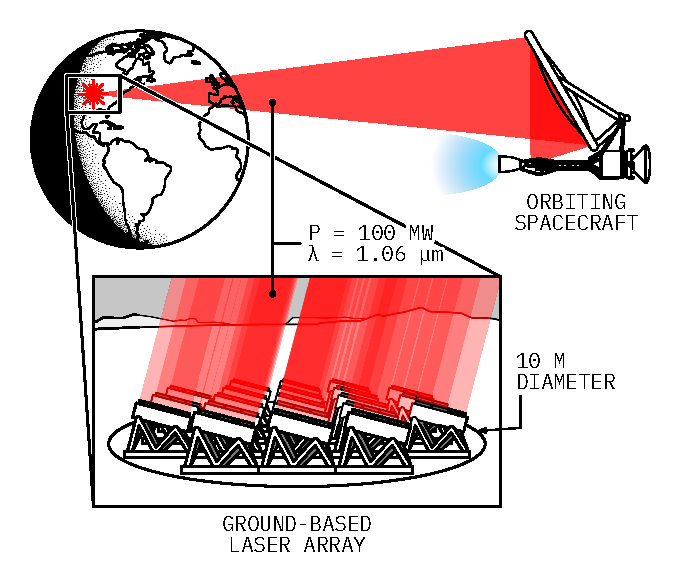
\includegraphics[width=0.4\textwidth]{assets/2 background/ltp_architecture.pdf}
            \caption{LTP architecture (\textcite{duplayArgonLaserPlasmaThruster2024a})}
            \label{fig:LTP architecture}
        \end{figure}

        In the thrust chamber of the vehicle, hydrogen is introduced. The laser is focused inside the chamber and is absorbed by the gas via inverse Bremsstrahlung, creating a Laser-Supported Plasma (LSP) core. Colder hydrogen flows around the LSP core and is heated by it to \qty{10000}{K}. The hot gas is then exhausted though a conventional converging-diverging nozzle at the exhaust velocity, imparting thrust to the vehicle.

        \begin{figure}[!ht]
            \centering
            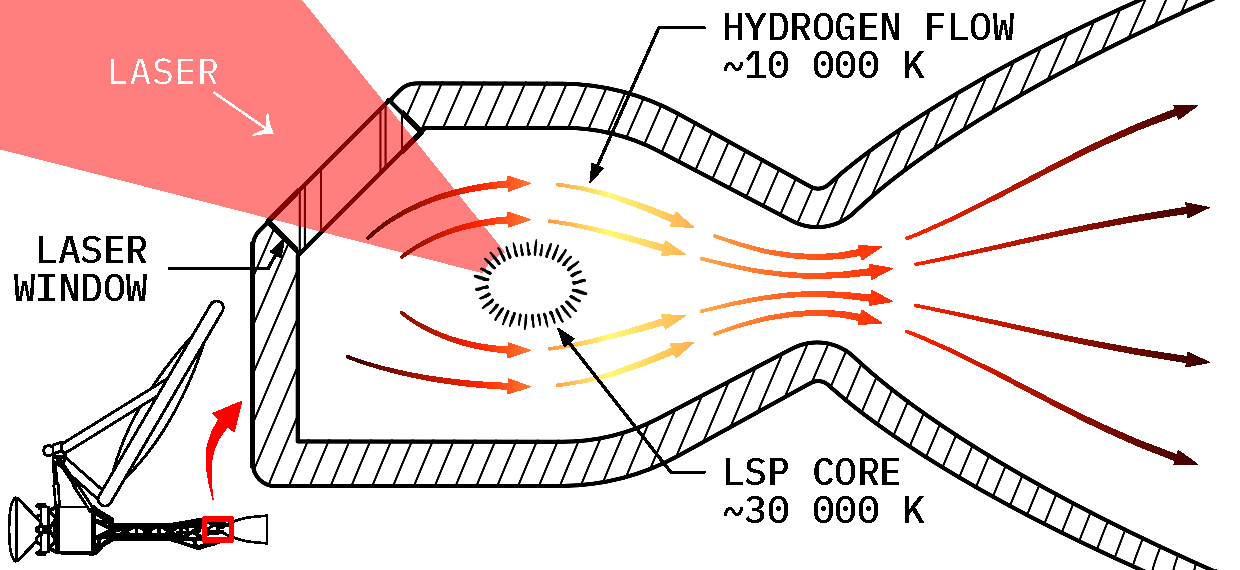
\includegraphics[width=0.6\textwidth]{assets/2 background/chamber.pdf}
            \caption{Overview of LTP system (\textcite{duplayArgonLaserPlasmaThruster2024a})}
            \label{fig:LTP system overview}
        \end{figure}

        In a conventional chemical rocket engine, the energy source is the oxidizer and the fuel, which are reacted together to release energy. They are transported with the rocket and set the temperature of the combustion reaction (typically \qtyrange{2000}{3000}{K}), which is directly related to the exhaust velocity.
        
        Separating the power source used for propulsion (here, the laser) from the spacecraft itself allows crucial weight savings, either increasing the payload mass fraction or decreasing transit time. Using a laser also allows for much greater thrust chamber temperatures than chemical propulsion, as the temperature of these plasmas is typically \qtyrange{15000}{30000}{K}. This gives in turn greater exhaust velocities. This propulsion method could therefore be an order of magnitude more efficient than our current rocket engines if certain engineering problems can be solved.

        Increasing the amount of energy deposited by the laser into the working gas remains a topic of active research and is a significant hurdle for the operational use of LTP. The two main conversion efficiencies are:
        \begin{enumerate}
            \item Absorption of the laser energy by the plasma
            \item Heat transfer from the plasma to the working gas (e.g. propellant)
        \end{enumerate}
        A selection of past LSP experiments will now be presented, with an emphasis on these efficiencies. As the efficiencies chosen are different from source to source, these will be defined where applicable.
    
    \section{Literature review}

        %Russian work: 1960s-2000s?

        The experimental basis of LTP was developed by \textcite{generalovContinuousOpticalDischarge1970} in 1970. For the first time, an LSP was generated with a \qty{150}{W} \ce{CO2} laser operating at \qty{10.6}{μm} wavelength. In this case, the LSP was initiated by a second, \qty{10}{kW} pulsed \ce{CO2} laser.
        
        %American work: 1970s-1990s?

        Work was done in the mid-1970s by \textcite{shojiLaserheatedRocketThruster1977,shojiPerformanceHeatTransfer1976a} to design a small-scale \qty{10}{kW} and full-scale \qty{5000}{kW} LTP engine. Carbon-seeded hydrogen was chosen to capture the plasma's radiation, which was mostly in the UV wavelength. \qty{20}{\%} of the laser power would be lost by convection and radiation to the walls in the \qty{10}{kW} thruster, with an additional \qty{5}{\%} of laser power lost by radiation through the thruster window. However, this was not tested. The \qty{10}{kW} prototype (\autoref{fig:Shoji apparatus}) was built and delivered to NASA at the conclusion of their effort.
        \begin{figure}[!ht]
            \centering
            \begin{subfigure}[t]{0.45\textwidth}
                \centering
                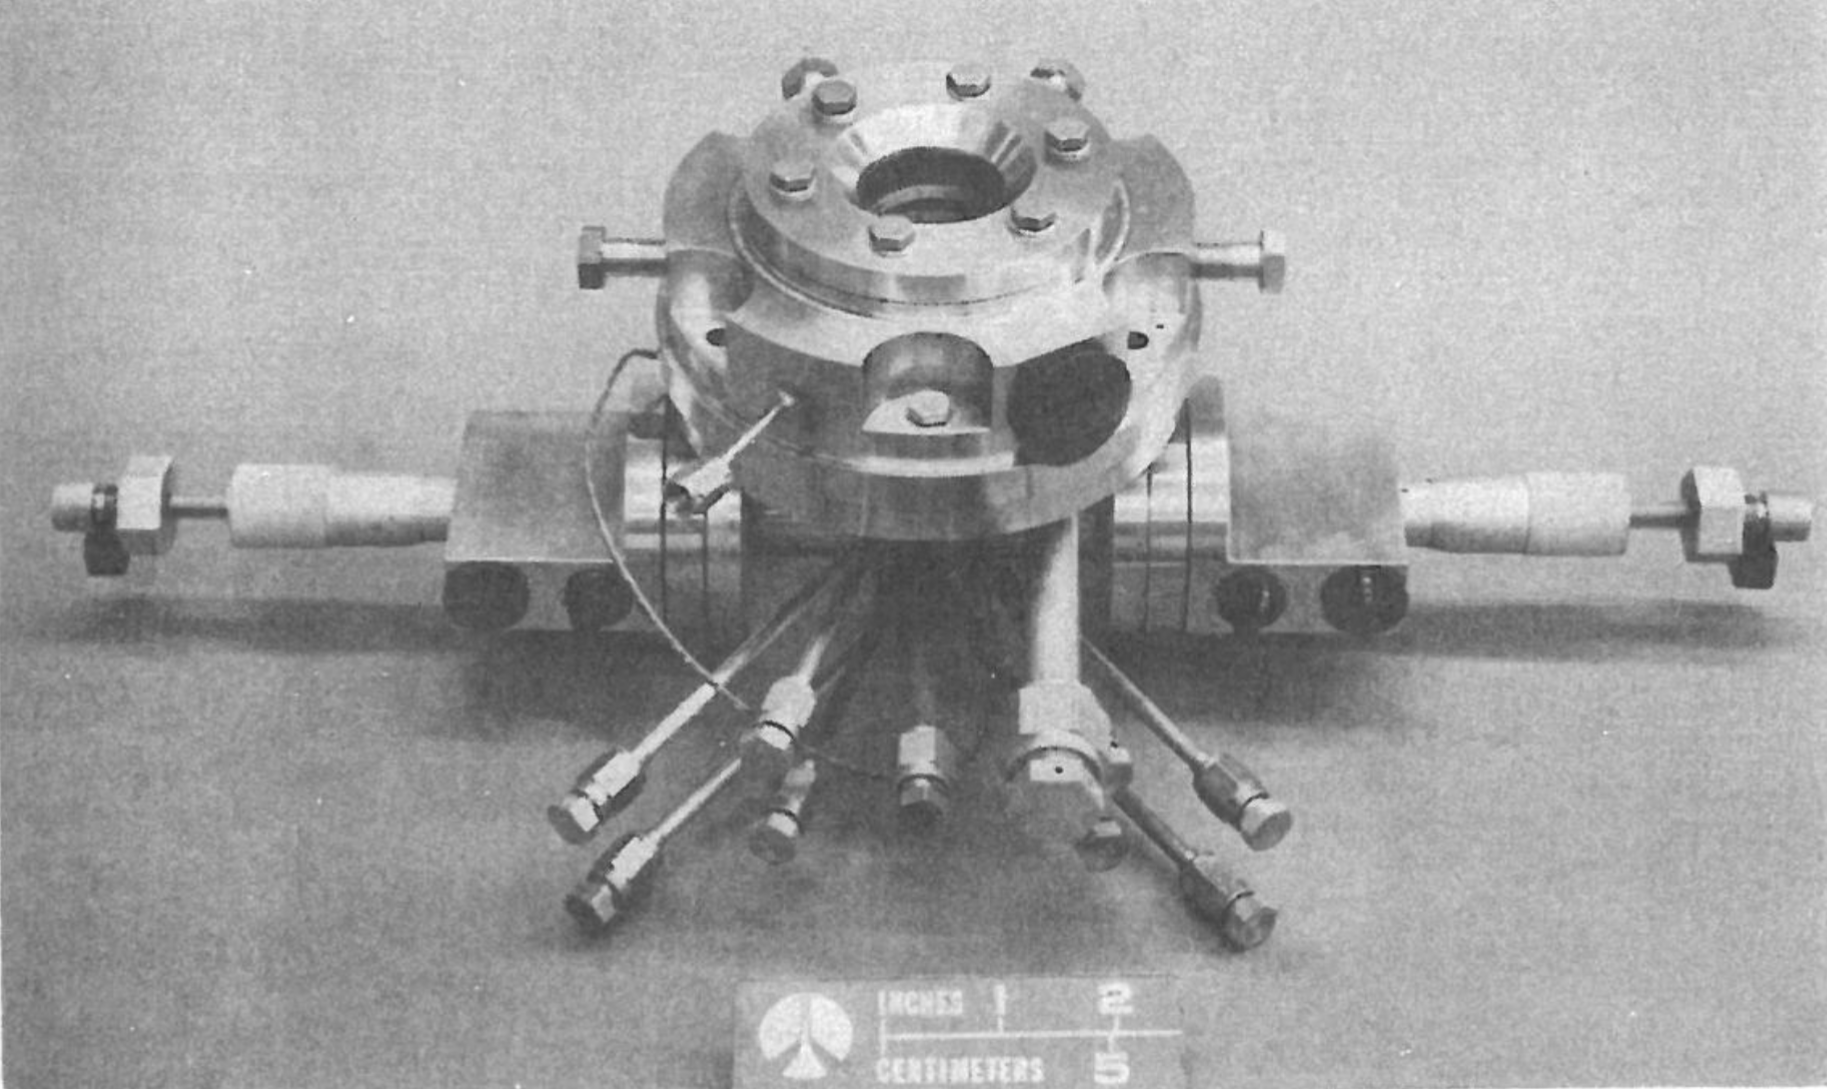
\includegraphics[width=\textwidth]{assets/2 background/Shoji_assy.png}
                \caption{\qty{10}{kW} thruster from \textcite{shojiPerformanceHeatTransfer1976a}}
                \label{fig:Shoji apparatus}
                \end{subfigure}
            \hfill
            \begin{subfigure}[t]{0.45\textwidth}
                \centering
                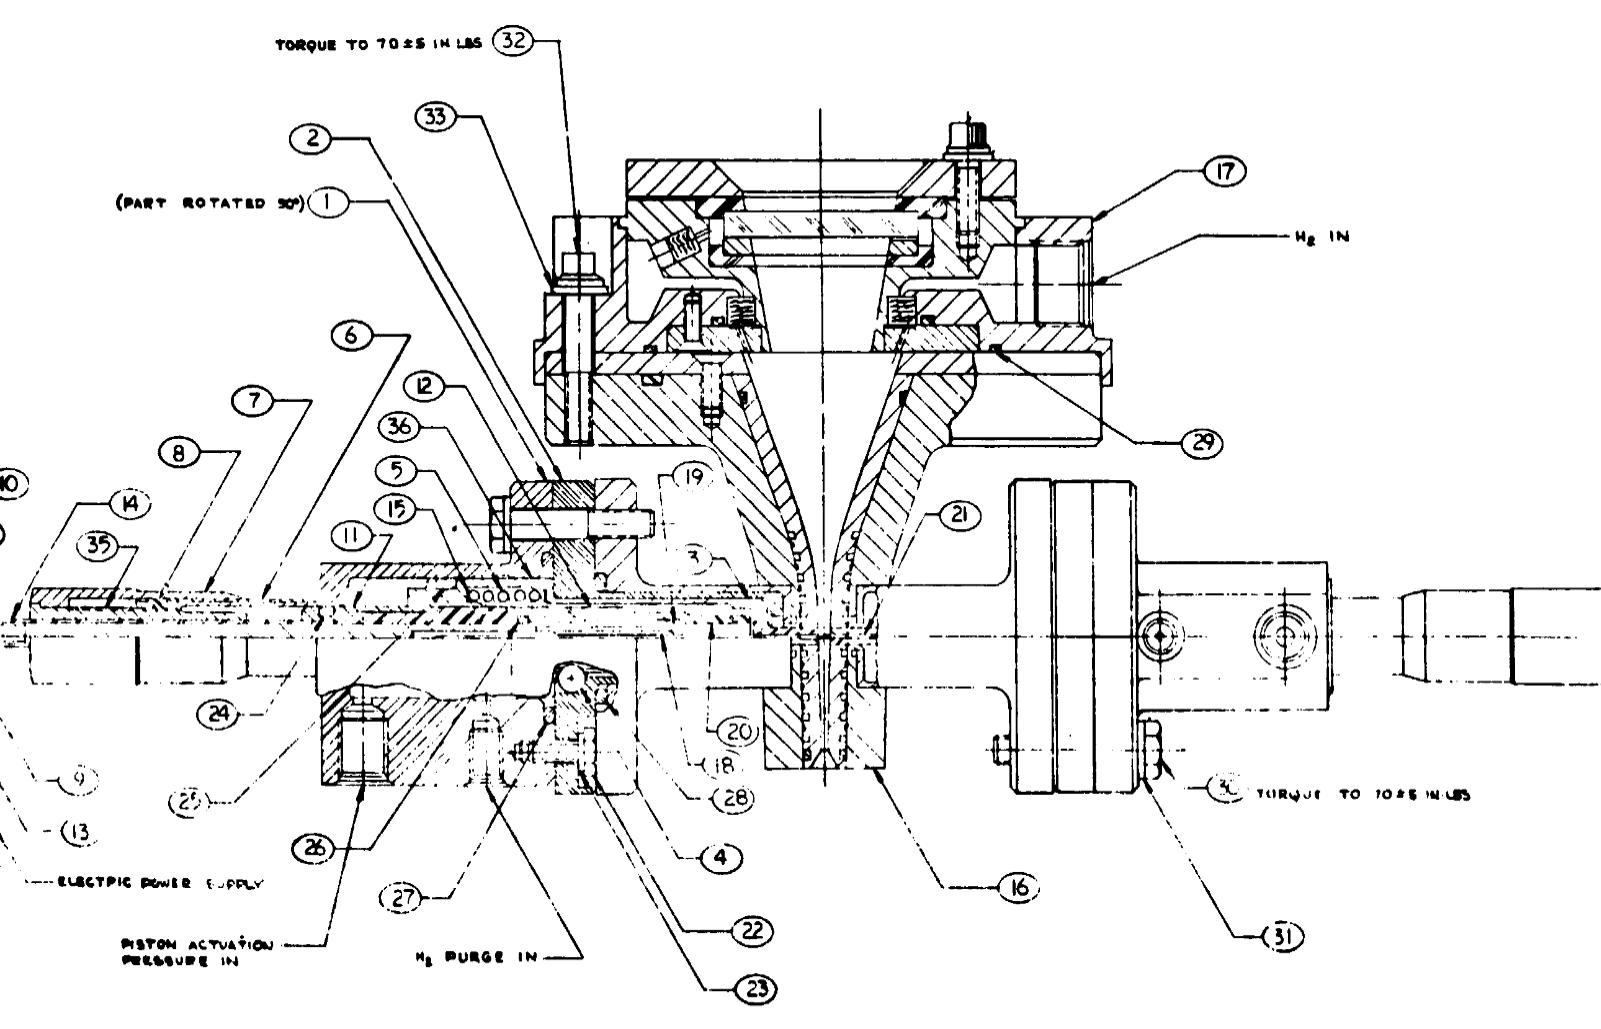
\includegraphics[width=\textwidth]{assets/2 background/Shoji cross-section.png}
                \caption{Cross-section drawing of \qty{10}{kW} thruster from \textcite{shojiLaserheatedRocketThruster1977} (original is of poor quality)}
                \label{fig:Shoji cross-section}
            \end{subfigure}
            \caption{Thruster designed by \textcite{shojiLaserheatedRocketThruster1977}}
            \label{fig:Shoji apparatussies}
        \end{figure}

        In the 1980s, \textcite{keeferPowerAbsorptionLasersustained1986a} studied LSP in a forced convective flow environment. Using a \qty{1.5}{kW} \ce{CO2} laser with power levels of \qtyrange{360}{840}{W} and pressures of \qtyrange{1.3}{2.3}{atm}, with varying argon flow velocities, the temperature field of the plasma was measured. From the temperature field, and assuming local thermodynamic equilibrium, the power absorbed by the plasma and the power radiated from it can be calculated.
        \begin{figure}[!ht]
            \centering
            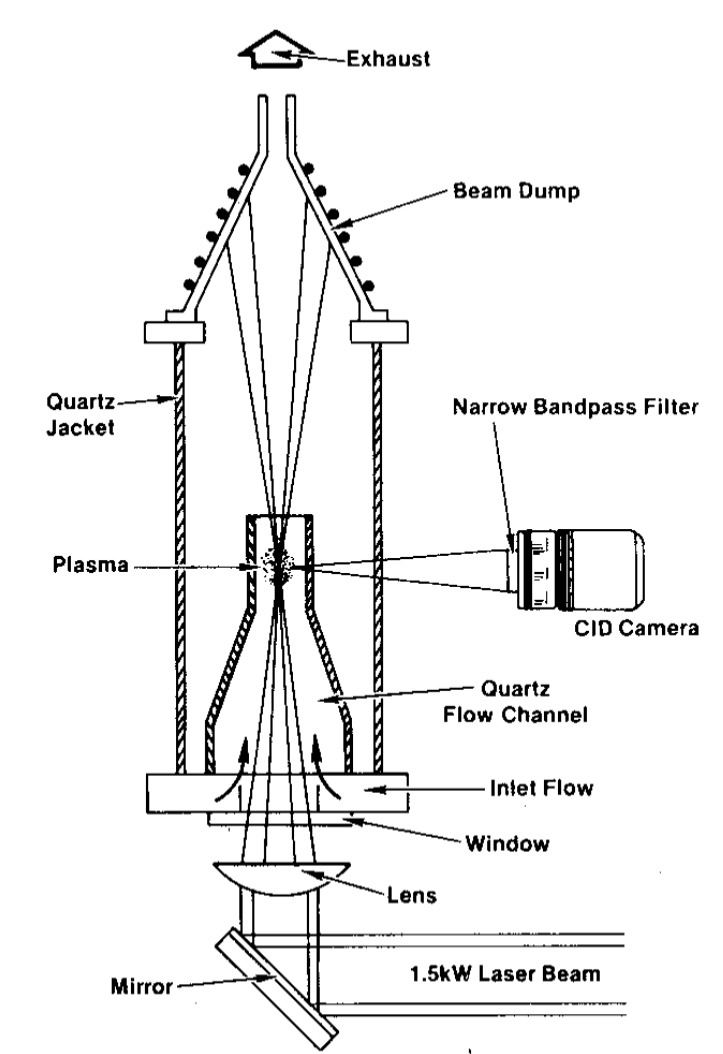
\includegraphics[width=0.4\textwidth]{assets/2 background/UTSI (Keefer) Apparatus.png}
            \caption{Experimental apparatus from \textcite{keeferPowerAbsorptionLasersustained1986a}}
            \label{fig:Keefer apparatus}
        \end{figure}
        \autoref{fig:Keefer apparatus} shows the apparatus used for these measurements. An inner quartz flow channel contained the plasma, while an outer quartz jacket contained the pressure. The plasma was initiated by laser heating of a tungsten rod, which was removed after initiation. Downstream, a water-cooled copper beam dump absorbed the energy of the laser and the heated argon flow, but was not used for measurements. The plasma's temperature was obtained through analyzing digital images. This temperature field was then used to calculate the power absorption and the radiation loss. The power absorbed by the plasma was between \qtyrange{23}{61}{\%} of incident laser power, while radiation loss was between \qtyrange{51}{80}{\%} of the absorbed power.

        Contemporary to \textcite{keeferPowerAbsorptionLasersustained1986a}, Mazumder and Krier headed a group at the University of Illinois that advanced the field of LTP. \textcite{krierContinuousWaveLaser1986a} reported laser absorption in an argon plasma approaching \qty{80}{\%}. \autoref{fig:Krier apparatus} shows the apparatus that was used by \textcite{krierContinuousWaveLaser1986a}, \textcite{zerkleLasersustainedArgonPlasmas1990} and \textcite{chenEmissionSpectroscopyCw1989a}. This vertical cylindrical flow chamber was made of 304 steel and had an internal diameter of 5 inches. A water-cooled calorimeter was used as a beam dump for the \qty{10}{kW} \ce{CO_2} laser. The laser energy not collected by the beam dump was assumed to be absorbed by the plasma, as the radiation reflected off the plasma is less than \qty{2}{\%} at these electron number densities. Moveable thermocouples gave two-dimensional maps of the flow surrounding the plasma core. The direct laser heating of the thermocouples and their carriage was taken into account.
        \begin{figure}[!ht]
            \centering
            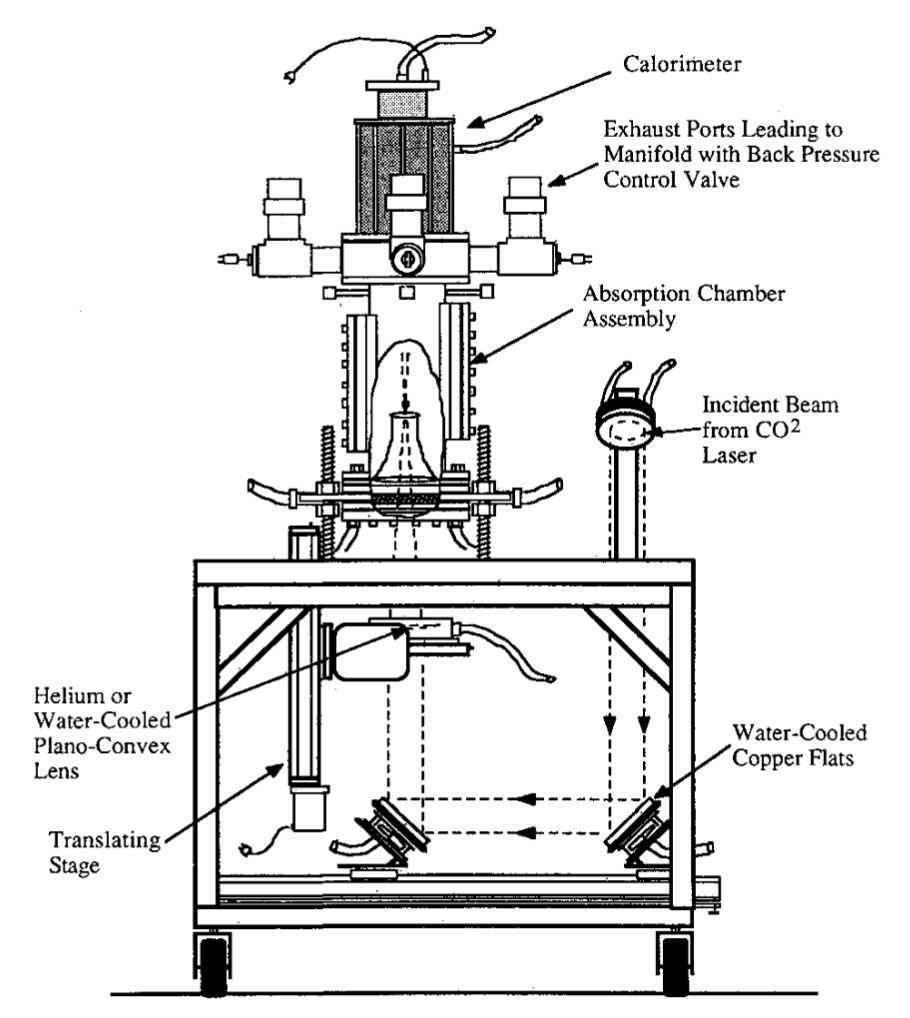
\includegraphics[width=0.5\textwidth]{assets/2 background/Illinois (Krier) Apparatus.png}
            \caption{Experimental apparatus from \textcite{zerkleLasersustainedArgonPlasmas1990}}
            \label{fig:Krier apparatus}
        \end{figure}
        These two-dimensional temperature maps \todo{INSERT EXPLANATION HERE}. Thermal efficiency was between \qtyrange{6}{25}{\%}, with radiative losses of \qty{64}{\%} and \qty{30}{\%}, 
        respectively. Thermal efficiency was defined as:


        \[\eta_\mathrm{th} =  \frac{\text{Power retained by the gas}}{\text{Incident laser power}}\]
        The minimum maintenance intensity of the plasma was also estimated at \qtyrange{0.1}{0.3}{MW/cm^2}.

        Further work by \textcite{zerkleLasersustainedArgonPlasmas1990} with the apparatus shown in \autoref{fig:Krier apparatus} reported absorption from \qtyrange{55}{97}{\%} and thermal efficiency from \qtyrange{11}{46}{\%}. This was done in \qtylist{1 2.5}{atm} of flowing argon, with laser powers up to \qty{7}{kW}. \textcite{chenEmissionSpectroscopyCw1989a} again increased the thermal efficiency of this apparatus, with \qtyrange{41}{62}{\%} of the laser energy being retained by the gas as thermal energy. This was among the highest thermal efficiencies measured by an LSP experiment. Here, \qty{86}{\%} of the laser's energy is absorbed by the LSP. This was attained with a \qty{5}{kW} \ce{CO2} laser, with flow speeds between \qtyrange{2}{10}{m/s}. They discuss that greater thermal efficiency is due to greater laser power, a high enough flow speed and a greater laser focusing $f$ number.

        Based on work by the Illinois group, an LTP engine demonstrator was tested in 1995 by \textcite{blackLaserPropulsion10kW1995} with a \qty{10}{kW} \ce{CO2} laser. This was planned to be a step towards a full-scale thruster. More than 100 thruster firings were completed, lasting 1 to 2 minutes each. The \qty{10}{kW} thruster is presented in \autoref{fig:Black apparatus}. It is mounted in a vacuum chamber to a thrust measurement assembly. Efficiency was calculated from:
        \[ \eta = \frac{F^2}{2 \dot{m} P_\mathrm{L}} \]
        with $P_\mathrm{L}$ the input laser power at the thruster window. Both argon and hydrogen were used. Argon propellant produced \qty{200}{s} of $I_\mathrm{sp}$ and a peak efficiency of 0.24. With hydrogen propellant, an $I_\mathrm{sp}$ of \qty{350}{s} and a peak efficiency of 0.37 were reported.
        \begin{figure}[!ht]
            \centering
            \begin{subfigure}[t]{0.3\textwidth}
                \centering
                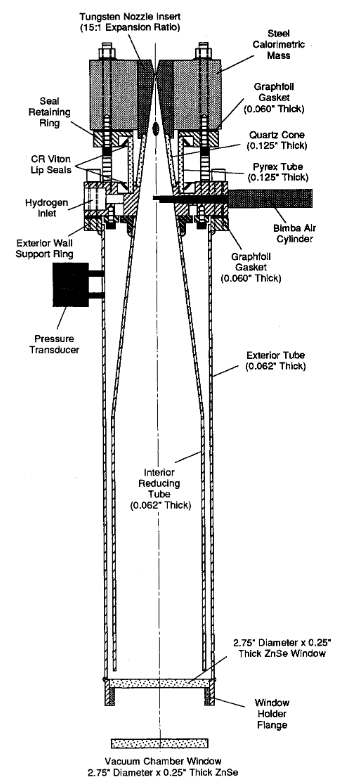
\includegraphics[width=\textwidth]{assets/2 background/BlackKrier thruster.png}
                \caption{\qty{10}{kW} thruster}
                \label{fig:Black apparatus}
            \end{subfigure}
            \hfill
            \begin{subfigure}[t]{0.45\textwidth}
                \centering
                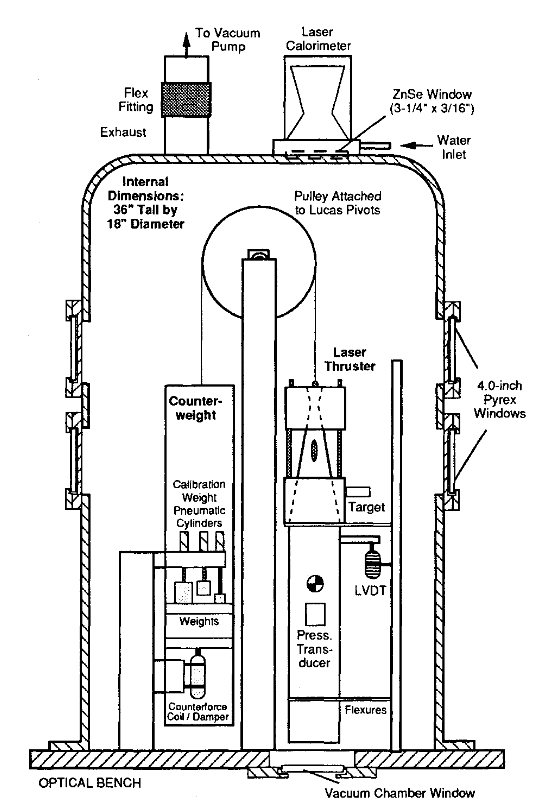
\includegraphics[width=\textwidth]{assets/2 background/Black thrust measurement assy.png}
                \caption{Thrust measurement assembly}
                \label{fig:Black thrust measurement}
            \end{subfigure}
            \caption{Apparatus used in \textcite{blackLaserPropulsion10kW1995}}
            \label{fig:Black apparatussies}
        \end{figure}
        A preliminary design for the full-scale \qty{100}{kW} thruster was also presented, with a predicted specific impulse of \qty{1000}{s}, thrust of \qty{4.5}{N} and a conversion efficiency of \qty{80}{\%}.

        %Chinese and Japanese work: 1980s-2020s

        In the early 2000s, \textcite{toyodaThrustPerformanceCW2002} built and tested two different thruster models, presented in \autoref{fig:Toyoda apparatussies}. These thrusters, using argon or nitrogen heated by LSP, were powered by a \qty{2}{kW} \ce{CO2} laser. The LSPs were initiated by a retractable tungsten rod at the laser's focus. Thrust measurements were done both in atmospheric pressure and in vacuum. This comparative study showed that confining the plasma into a smaller chamber increased heat transfer and therefore, efficiency. \textcite{toyodaThrustPerformanceCW2002} defined the energy conversion efficiency as the amount of laser power that is converted into usable kinetic energy for thrust. It is calculated as\footnote{As mentioned by \textcite{duplayArgonLaserPlasmaThruster2024a}, there appears to be a typographical error in the reference as the units are inconsistent. The corrected equation is presented here.}:
        \[ \eta_\mathrm{e} =  \frac{F^2_\mathrm{hot} -F^2_\mathrm{cold}}{2 \dot{m} P}\]
        Where $F_\mathrm{hot}$ is the thrust with laser on, $F_\mathrm{cold}$ is the cold flow thrust (laser off) and $P$ is incident laser power. An energy conversion efficiency of 37\% and an $I_\mathrm{sp}$ of \qty{113}{s} were measured with the second model \autoref{fig:Toyoda apparatus 2} in vacuum with argon propellant. The pressure ratio, defined as the chamber pressure divided by the nozzle exit pressure, was 420. A water cooling system measured the heat loss to the walls to be 55\% of incident laser power, with a final 8\% being ``other loss". Heat loss to the walls was expected to be recycled with regenerative cooling in a real-world application.

        \begin{figure}[!ht]
            \centering
            \begin{subfigure}[t]{0.45\textwidth}
                \centering
                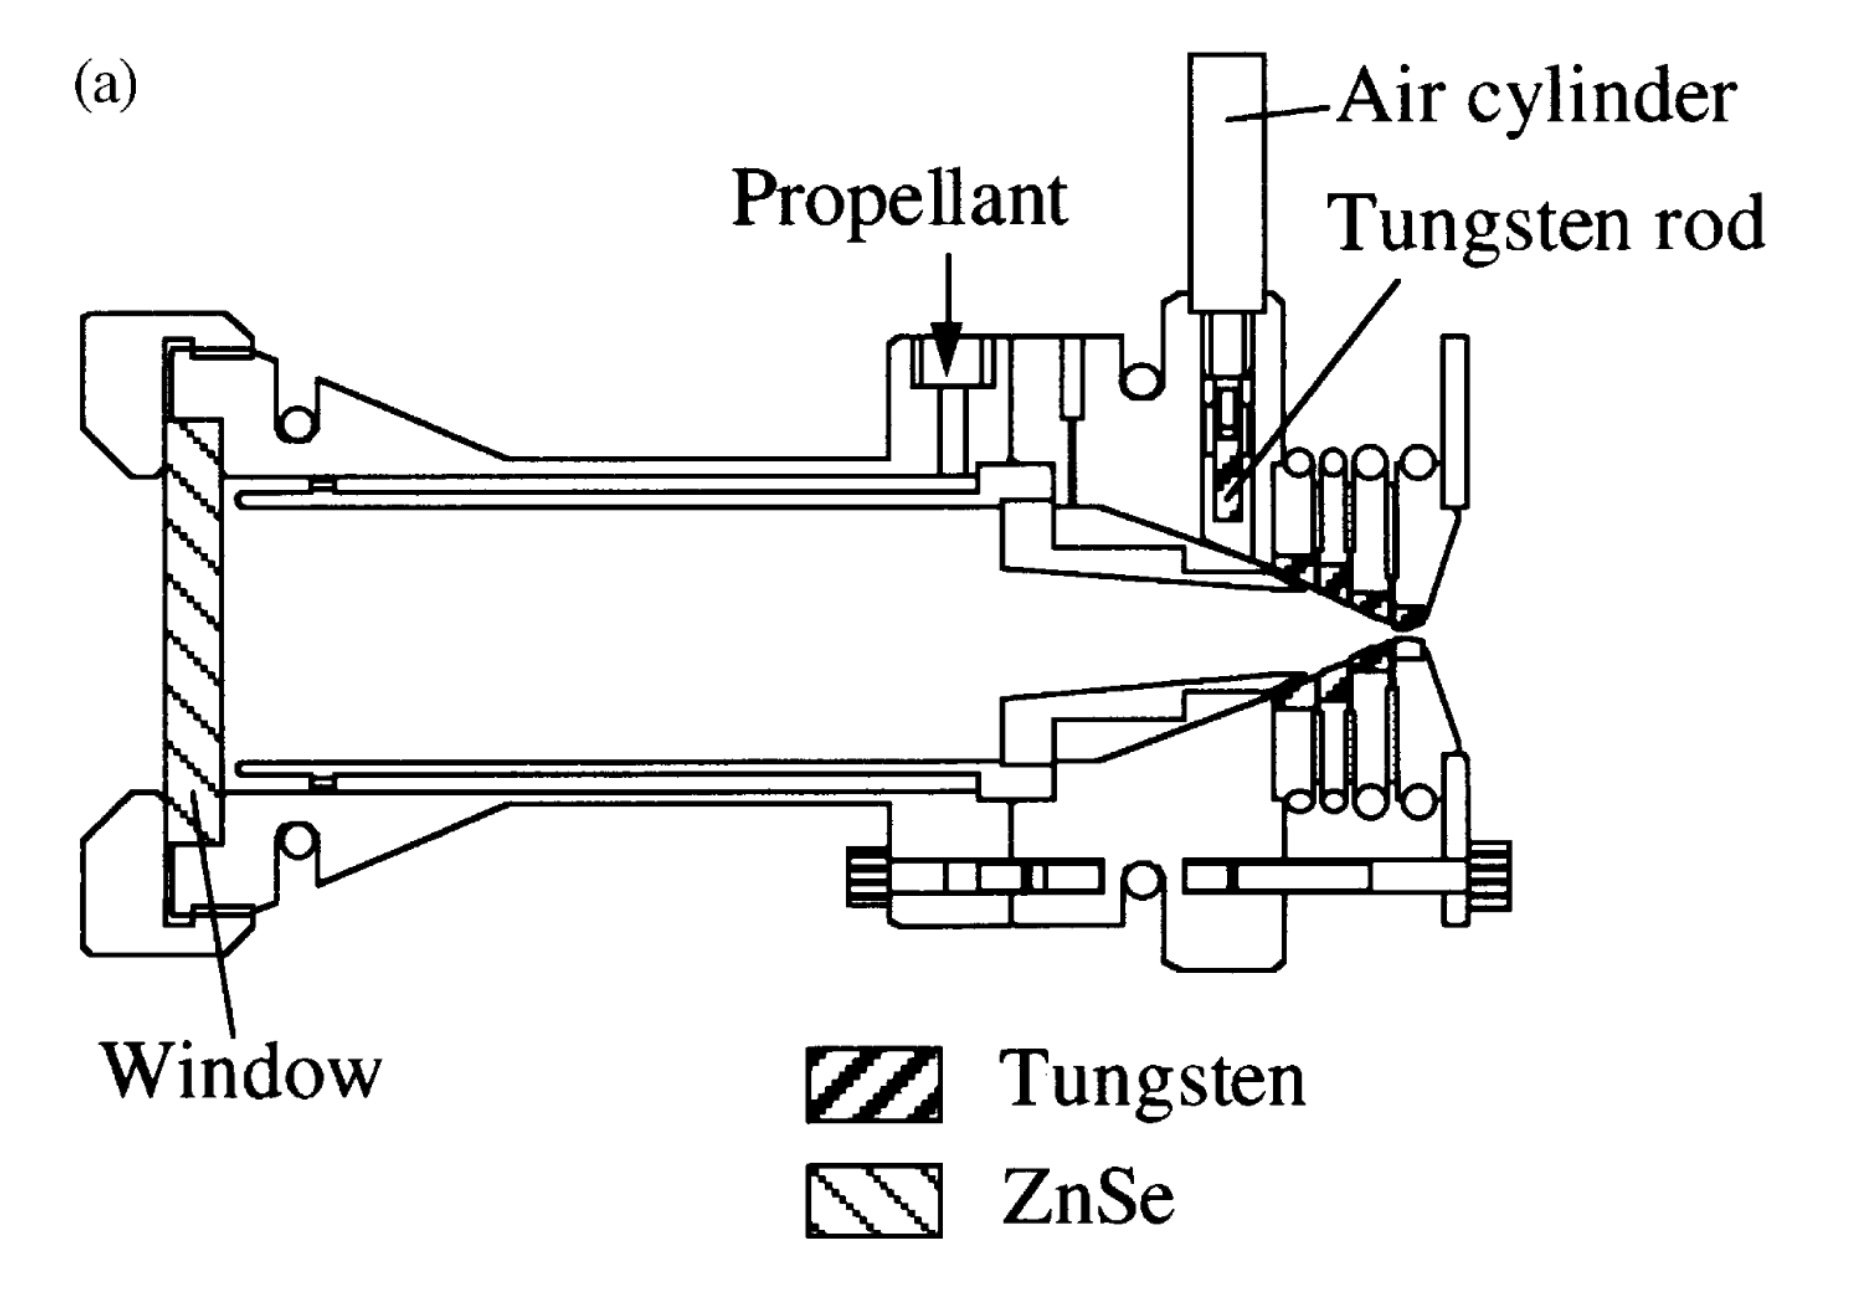
\includegraphics[width=\textwidth]{assets/2 background/Toyoda apparatus model 1.jpg}
                \caption{Model I}
                \label{fig:Toyoda apparatus 1}
            \end{subfigure}
            \hfill
            \begin{subfigure}[t]{0.45\textwidth}
                \centering
                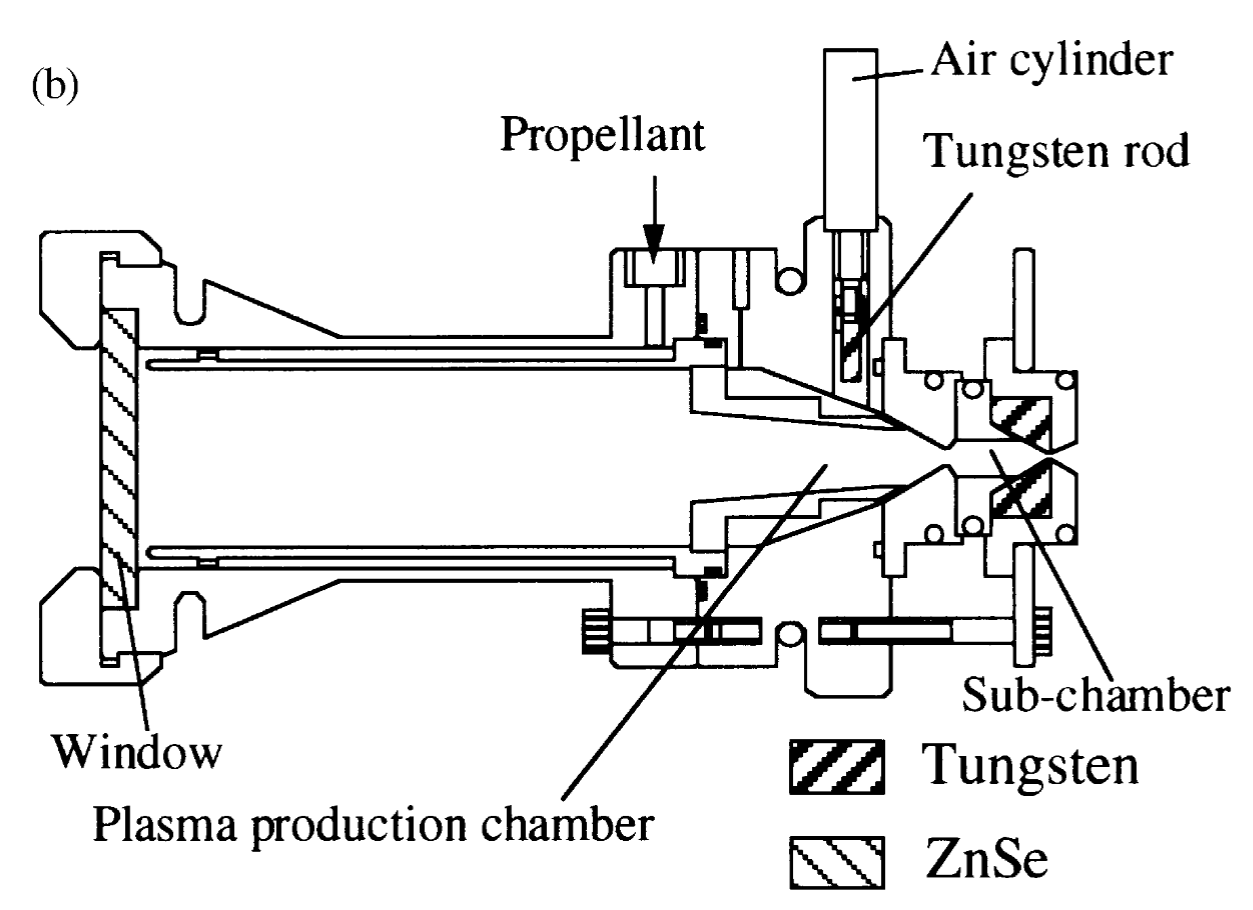
\includegraphics[width=\textwidth]{assets/2 background/Toyoda Apparatus model 2.png}
                \caption{Model II}
                \label{fig:Toyoda apparatus 2}
            \end{subfigure}
            \caption{Two thruster models from \textcite{toyodaThrustPerformanceCW2002}}
            \label{fig:Toyoda apparatussies}
        \end{figure}

        \textcite{luCharacteristicDiagnosticsLaserStabilized2022a} investigated LSP for lighting applications instead of propulsion. Therefore, an emphasis was made on spectroscopy measurements. A \qty{300}{W} fiber laser at a wavelength of \qty{1080}{nm} was focused to a \qty{50}{μm} diameter spot in a high pressure chamber.
        \begin{figure}[!ht]
            \centering
            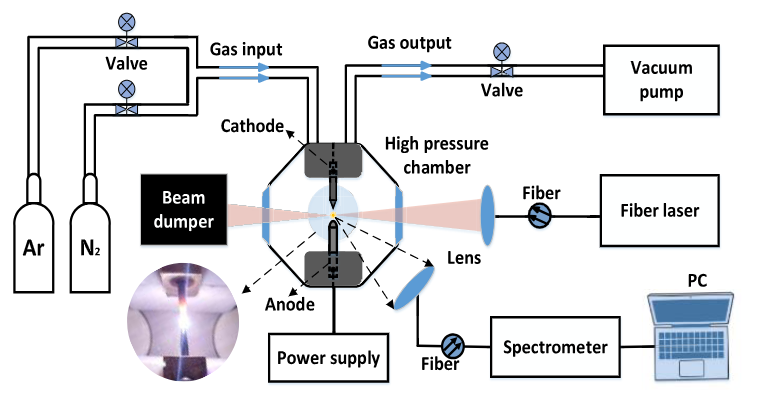
\includegraphics[width=0.7\textwidth]{assets/2 background/Lu apparatus.png}
            \caption{Experimental setup from \textcite{luCharacteristicDiagnosticsLaserStabilized2022a}}
            \label{fig:Lu apparatus}
        \end{figure}
        Argon was used, with pressures between \qtyrange{10}{20}{bar}. A lower initiation power (\qty{117}{W}) than other studies was achieved at \qty{20}{bar}. This was attributed to the smaller focus delivering a greater photon flux. \ce{N2} was later added between \qtyrange{0.1}{1.0}{\%}. As expected, increasing the laser power or the gas pressure was found to increase the radiation intensity of the LSP. However, adding \ce{N2} reduced both the electron temperature and electron density of the LSP, reducing its radiation intensity.

        Seeding the working gas with another species has been discussed as a way to increase the energy absorption into the working fluid of an LTP engine. LSPs in pure methane and methane-seeded gasses have been investigated by \textcite{kameiMethaneMethaneXenon2020}. Methane dissociates into hydrogen and carbon with the high temperature of the LSP. As mentioned with \textcite{shojiLaserheatedRocketThruster1977}, carbon particles would absorb the LSP's UV radiation.  A \qty{1.1}{kW} diode laser at a wavelength of \qty{940}{nm} was beamed into a high-pressure chamber fitted with arc initiation electrodes. The gap between these electrodes was \qty{1}{mm}. A CCD type spectrometer recorded emission spectra of the initiation arc discharge and of the LSP. LSPs in three different gasses were attempted: pure methane, methane-argon, and methane-xenon.
        
        In methane at \qty{0.1}{MPa}, soot formation between the electrodes prevented LSP initiation. The spectrometer confirmed the dissociation of methane, as line spectra of carbon and hydrogen were observed at the initiation arc. Initiation was also unsuccessful in argon-methane with a pressure between \qtyrange{0.1}{0.3}{MPa} and a methane volume fraction between \qtyrange{20}{60}{\%}. LSP was successfully generated in methane-xenon, with a lower threshold power (\qty{850}{W}) than in pure xenon. The partial pressure of methane was between \qtyrange{0.02}{0.6}{MPa}, with a partial pressure of xenon of \qty{0.10}{MPa}.

        \textcite{takanoDemonstrationDiodeLasersustained} used a diode laser emitting simultaneously at \qty{927}{nm} and \qty{951}{nm} to generate LSPs in argon. This resulted in an $I_\mathrm{sp}$ of \qty{105}{s} and a thrust efficiency of \qty{8}{\%}. This $I_\mathrm{sp}$ was calculated from the plenum pressure when the laser was on. They define thrust efficiency as:
        \[
        \eta = \frac{g_0 I_\mathrm{sp} (F_\mathrm{hot}-F_\mathrm{cold})}{2 P_\mathrm{laser}}
        \]
        Two setups were used: the LSP generation chamber previously used by \textcite{kameiMethaneMethaneXenon2020} (\autoref{fig:Takano LSP generation chamber}) and an LSP thruster (\autoref{fig:Takano LSP thruster}).
        \begin{figure}[!ht]
            \centering
            \begin{subfigure}[t]{0.45\textwidth}
                \centering
                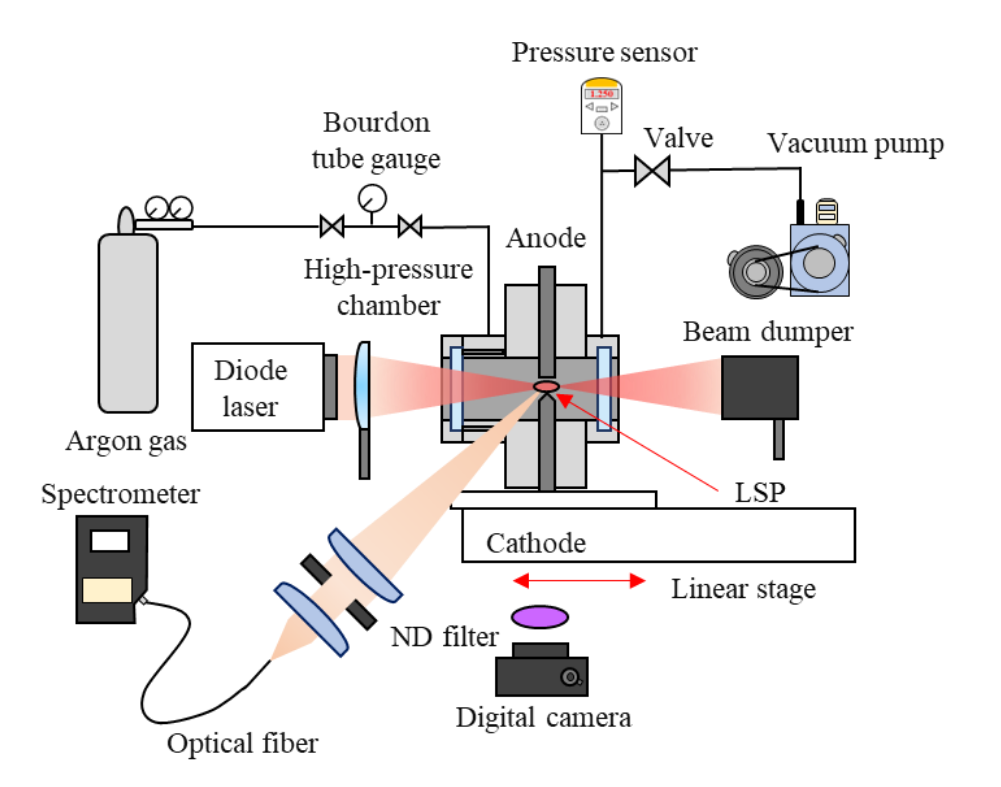
\includegraphics[width=\textwidth]{assets/2 background/Takano LSP chamber.png}
                \caption{LSP generation chamber and systems}
                \label{fig:Takano LSP generation chamber}
            \end{subfigure}
            \hfill
            \begin{subfigure}[t]{0.45\textwidth}
                \centering
                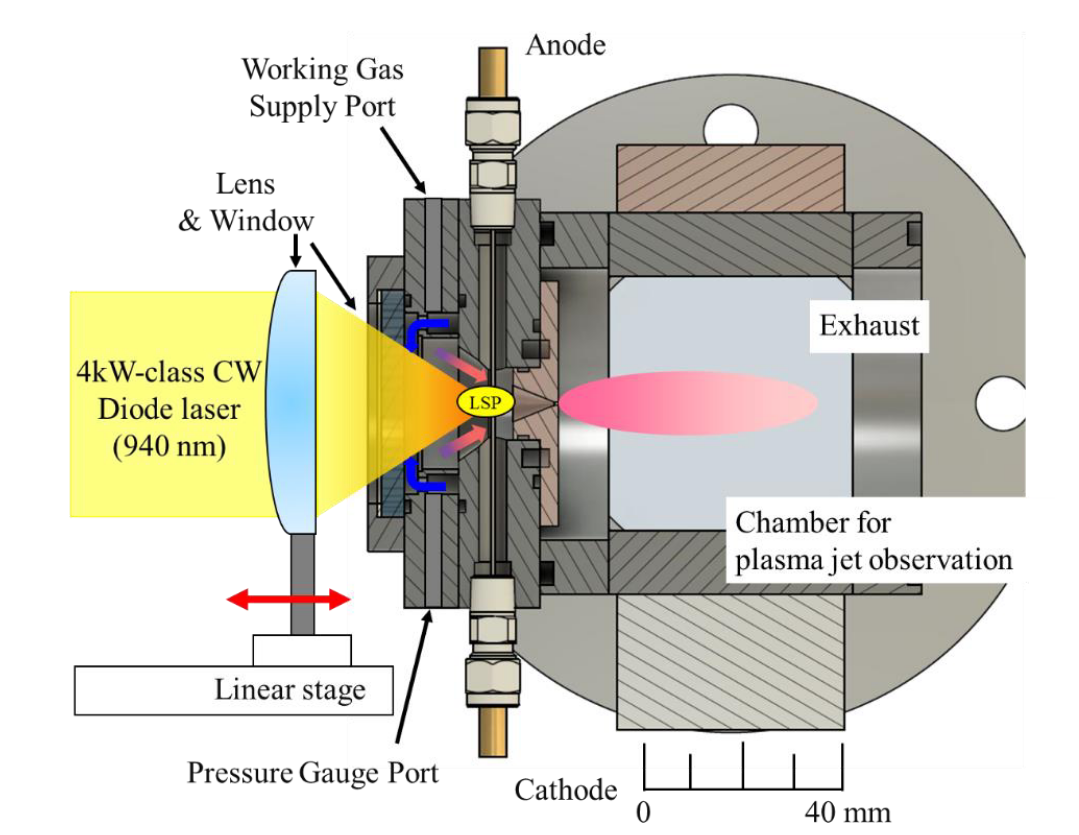
\includegraphics[width=\textwidth]{assets/2 background/Takano LSP thruster.png}
                \caption{LSP thruster}
                \label{fig:Takano LSP thruster}
            \end{subfigure}
            \caption{LSP setups from \textcite{takanoDemonstrationDiodeLasersustained}}
            \label{fig:Takano apparatussies}
        \end{figure}
        The LSP chamber was used to determine the effect of various F-numbers on the argon LSP. The thruster has an interchangeable copper throat, with diameters of \qty{0.7}{mm} and \qty{1.0}{mm}. In both setups, electric arc initiation was used. Once initiated in the thruster, the LSP is moved toward the nozzle with the lens mounted on a motorized stage. It was found that moving the LSP this way increased the heat exchange with the working gas. Thrust was calculated by using the pressure measurements inside the thruster's heating chamber.

        %Canadian work: 2020s  

        \textcite{duplayArgonLaserPlasmaThruster2024a} used a \qty{3}{kW} pulsed fiber laser to create LSPs in static and flowing argon. In static argon, about \qty{80}{\%} of the laser energy was being absorbed by the plasma, with approximately \qty{15}{\%} of the laser energy heating the bulk gas. This was done between \qtyrange{5}{20}{bar}.
        \begin{figure}[!ht]
            \centering
            \includegraphics[width=0.7\textwidth]{assets/2 background/finalsetup_static.pdf}
            \caption{Static LSP apparatus from \textcite{duplayArgonLaserPlasmaThruster2024a}}
            \label{fig:Duplay apparatus}
        \end{figure}

    \section{Summary and direction of work in this thesis}
        
        From the literature review, \autoref{tab:lit review summary} and \autoref{tab:efficiencies} were compiled. Most studies have used \ce{CO2} lasers with a wavelength of \qty{10.6}{μm}. Use of a \ce{CO2} laser for power beaming to a remote target for propulsion applications is limited by the range over which the laser can be focused due to their long laser wavelength. 
    
        Indeed, the diffraction limit of a laser, which is the theoretical lower limit on beam divergence, equals the wavelength ($\lambda$) divided by the diameter $D$ of the output beam \cite{hechtUnderstandingLasersEntry2019}.
        \[
        \text{Diffraction limit (radians)} = \lambda/D
        \]
        This relegated \ce{CO2} lasers to ground-to-orbit launch. Recently, high power fiber lasers emitting near \qty{1}{μm} have become readily available. Being able to beam energy to low earth orbit, fiber lasers make laser propulsion more feasible.

        \begin{table}[!ht]
            \centering
            \caption{Summary of a selection of past LSP experiments. $\lambda$: wavelength, $P$: maximum laser power, $p$: pressure, $\dot m$: mass flow rate, $I_\mathrm{sp}$: maximum specific impulse, $F_\mathrm{T}$: maximum thrust}
            \label{tab:lit review summary}
            \begin{tabularx}{\textwidth}{@{}>{\small}X<{\raggedright}lXXrXXXrr<{\raggedright}@{}}
            \toprule
            {\normalsize LSP   Facility} & Year & Laser & $\lambda$ [\unit{\um}] & $P$ [kW] & Gas & $p$ [atm] & $\dot m$ [g/s] & $I_\mathrm{sp}$ [s] & $F_\mathrm{T}$ [N]  \\ \midrule
            \textcite{generalovContinuousOpticalDischarge1970}        &1970&\ce{CO_2}&10.60&0.15 &\ce{Xe}           & 3.0-4.0  &  -  & -   &  -   \\
            \textcite{keeferPowerAbsorptionLasersustained1986a}       &1986&\ce{CO_2}&10.60&0.84 &\ce{Ar}           & 1.3-2.3  & 0.01-0.19   & -   &  -   \\
            \textcite{krierContinuousWaveLaser1986a}                  &1986&\ce{CO_2}&10.60&10  &\ce{Ar}           &     -       & 2.3-4.6 & -& -\\
            \textcite{zerkleLasersustainedArgonPlasmas1990}           &1988&\ce{CO_2}&10.60&7   &\ce{Ar}           &      -      &     -     & -&- \\
            \textcite{chenEmissionSpectroscopyCw1989a}                &1989&\ce{CO_2}&10.60&5   &\ce{Ar}           &      -      &  -  & -   & -    \\
            \textcite{blackLaserPropulsion10kW1995}                   &1995&\ce{CO_2}&10.60&10  &\ce{Ar}           & 1.4-2.4  & 5.1-9.4 & 200 & 7 \\
                                                                      &    &\ce{CO_2}&10.60&10  &\ce{H_2}          &    3.4        & 1.1&  350   & 3 \\
            \textcite{toyodaThrustPerformanceCW2002}                  &2002&\ce{CO_2}&10.60&2   &\ce{Ar}, \ce{N_2} & 2.0-5.5  &  -  & 113 & 0.44 \\
            \textcite{luCharacteristicDiagnosticsLaserStabilized2022a}&2022&Fiber    &1.08 &0.30 &\ce{Ar}, \ce{N_2} & 9.9-19.7 &  -  & -   & -    \\ 
            \textcite{takanoDemonstrationDiodeLasersustained}         &2024&Diode    &0.927 and 0.951 &4.4 &\ce{Ar}   & 10-15 &   - & 105   & -    \\
            \textcite{duplayArgonLaserPlasmaThruster2024a}            &2024&Fiber    &1.07  & 3 &\ce{Ar}            &   5-20  & 0 & - & - \\
            \bottomrule
            \end{tabularx}
        \end{table}

        \begin{table}[!ht]
            \centering
            \caption{Comparative table of experimental LTP thruster efficiencies}
            \label{tab:efficiencies}
            \begin{tabularx}{\textwidth}{@{}>{\small}X<{\raggedright} r l r@{}}
            \toprule
            {\normalsize LSP   Facility}   & Laser absorption  & Efficiency & Value of efficiency \\ \midrule
            \textcite{keeferPowerAbsorptionLasersustained1986a}   & 0.23 - 0.61      &          -        &                 -          \\
            \textcite{krierContinuousWaveLaser1986a}       & 0.50 - 0.80         & $\eta_\mathrm{th} =  \frac{\text{Power retained by the gas}}{\text{Incident laser power}}$ &  0.06 - 0.25 \\
            \textcite{zerkleLasersustainedArgonPlasmas1990}       & 0.55 - 0.97   &         $\eta_\mathrm{th} =  \frac{\text{Power retained by the gas}}{\text{Incident laser power}}$ &  0.11 - 0.46 \\
            \textcite{chenEmissionSpectroscopyCw1989a}          & 0.86                      &  $\eta_\mathrm{th} =  \frac{\text{Power retained by the gas}}{\text{Incident laser power}}$  &  0.41-0.62  \\
            \textcite{blackLaserPropulsion10kW1995}       &  -  & $ \eta = \frac{F_\mathrm{hot}^2}{2 \dot{m} P_\mathrm{L}} $& 0.20 - 0.25 (Ar), 0.25 - 0.40 (H)     \\
            \textcite{toyodaThrustPerformanceCW2002}    & -                      & $ \eta_\mathrm{e} =  \frac{F^2_\mathrm{hot} -F^2_\mathrm{cold}}{2 \dot{m} P} $     &   0.37 \\
            \textcite{takanoDemonstrationDiodeLasersustained}  &       -       & $ \eta = \frac{g_0 I_\mathrm{sp} (F_\mathrm{hot}-F_\mathrm{cold})}{2 P_\mathrm{laser}} $ & 0.08 \\ 
            \textcite{duplayArgonLaserPlasmaThruster2024a}  &  0.80&  $\eta_\mathrm{th} =  \frac{\text{Power retained by the gas}}{\text{Incident laser power}}$ & 0.15 \\
            \bottomrule
            \end{tabularx}
        \end{table}
        

        To increase thermal efficiency, \textcite{chenEmissionSpectroscopyCw1989a} suggest:
        \begin{enumerate}
            \item A greater laser power, which gives greater inverse bremsstrahlung absorption coefficient and longer absorption path length;
            \item A high enough flow speed to push the LSP back to the laser focus, but not too fast as to blow the plasma out;
            \item A greater laser focusing $f$ number, creating a longer and narrower plasma. This increases the probability a photon will be absorbed by the plasma and reduces the radiation loss.
        \end{enumerate}

        For a small-scale demonstration thruster, $I_\mathrm{sp}$ values near \qty{100}{s} can be expected, with thrust values under \qty{1}{N}, as was found by \textcite{toyodaThrustPerformanceCW2002} and \textcite{takanoDemonstrationDiodeLasersustained}.

        % Previous objective: The objective of this research project will be to test a lab-scale proof-of-concept LTP thruster for interplanetary space flight, using a \qty{1.07}{μm} fiber laser. Key performance parameters of this thruster such as thrust and specific impulse will be measured, and the LSP heating core inside the thruster will be characterized. 
        
        
        The objective of this research project will be to test a lab-scale proof-of-concept LTP thruster for interplanetary space flight, using a \qty{1.07}{μm} fiber laser \todo{add to this}. This project will mainly build upon the experimental research started by \textcite{duplayArgonLaserPlasmaThruster2024a}.
        
        % Link to next chapter, modelling c_p
        Before going into experiments, it is important to characterize certain thermodynamic properties of the gasses used. Notably, the modelling of heat capacity will be presented in the next chapter.

    \chapter{0D LSP Model} \label{chp:models}

    To predict experimental data, namely the pressure increase of the gas that should be expected when laser energy is input, the heat capacity of argon and hydrogen was modelled. A zero-dimensional (0D) heat transfer model was then written in Python to compare to experimental data. Argon and hydrogen were used to validate initial equilibrium calculations, while the 0D model was solely implemented using argon. Argon is the current gas used in experiments, as it is economical and easy to ionize. Hydrogen is projected to be used in a full-scale LTP engine for its increased $I_\mathrm{sp}$ due to its lower molecular weight.

    \section{Equilibrium calculations} \label{sec:equilibrium calcs}
        
        The following seventh order polynomials and their coefficients ($a_1$ to $a_7$, $b_1$, and $b_2$), from \textcite{mcbrideNASAGlennCoefficients2002}, were implemented in Python. Species of interest were \ce{H}, \ce{H2}, \ce{Ar}, \ce{Ar+}, and electrons \ce{e-}. Plasma temperatures studied allowed us to treat the argon as singly ionized, and the hydrogen as dissociated. The heat capacity at constant pressure, as well as the temperature ($T$) dependent part of enthalpy and entropy of each species are given by $c_p^0$, $h^0$ and $s^0$, respectively. $\bar R$ is the universal gas constant.

        \begin{equation}
            c_p^0 (T)/\bar R = a_1 T^{-2} + a_2 T^{-1} + a_3 + a_4   T + a_5 T^2 + a_6 T^3 + a_7 T^4
        \end{equation} 
        
        \begin{equation}
            h^0 (T)/\bar RT = -a_1 T^{-2} + a_2 \ln(T)/T + a_3 + a_4 T / 2 + a_5 {T^2}/3 + a_6 {T^3}/4 + a_7 {T^4}/5 + b_1/T
        \end{equation}
        
        \begin{equation}
            s^0(T)/\bar R = -a_1 T^{-2}/2 - a_2 T^{-1} + a_3\ln(T) + a_4   T + a_5 {T^2}/2 + a_6 T^3/3 + a_7 T^4/4 + b_2
        \end{equation}

        Next, the functions for entropy $\bar s_i$ of each species $i$ and Gibbs energy $\bar g_i$, both per \unit{kmol}, were implemented. These values depend on temperature $T$ and partial pressure $p_i$. $y_i$ is the molar fraction of the species, and $p_\mathrm{ref}$ is the reference pressure, equal to \qty{1}{bar}.
        
        \begin{equation}
            \bar s_i (T, p_i) = \bar s_i^0 (T) - \bar R \ln \frac{y_i p}{p_\mathrm{ref}}
        \end{equation}

        \begin{equation}
            \bar g_i = \bar h_i - T \bar s_i
        \end{equation}

        Considering the number of moles $n_i$, expressions of the Gibbs energy of the two mixtures $G_\mathrm{mixture}$ are found:

        Starting with \qty{1}{kmol} argon,
        \begin{equation}
            G_\mathrm{mixture,\: Ar}(T, p) = n_\mathrm{Ar} \bar g_\mathrm{Ar}(T, p_\mathrm{Ar}) + n_\mathrm{Ar+} \bar g_\mathrm{Ar+}(T, p_\mathrm{Ar+}) + n_\mathrm{e} \bar g_\mathrm{e}(T, p_\mathrm{e})
        \end{equation}

        Starting with \qty{1}{kmol} hydrogen,
        \begin{equation}
            G_\mathrm{mixture,\: H_2}(T, p) = n_\mathrm{H} \bar g_\mathrm{H}(T, p_H) + n_\mathrm{H2} \bar g_\mathrm{H2}(T, p_\mathrm{H2})
        \end{equation}

        \autoref{fig:Gibbs} plots the Gibbs energy of the hydrogen mixture as a function of its degree of dissociation $x$, for different total pressures $p$.

        \begin{figure}[!ht]
            \centering
            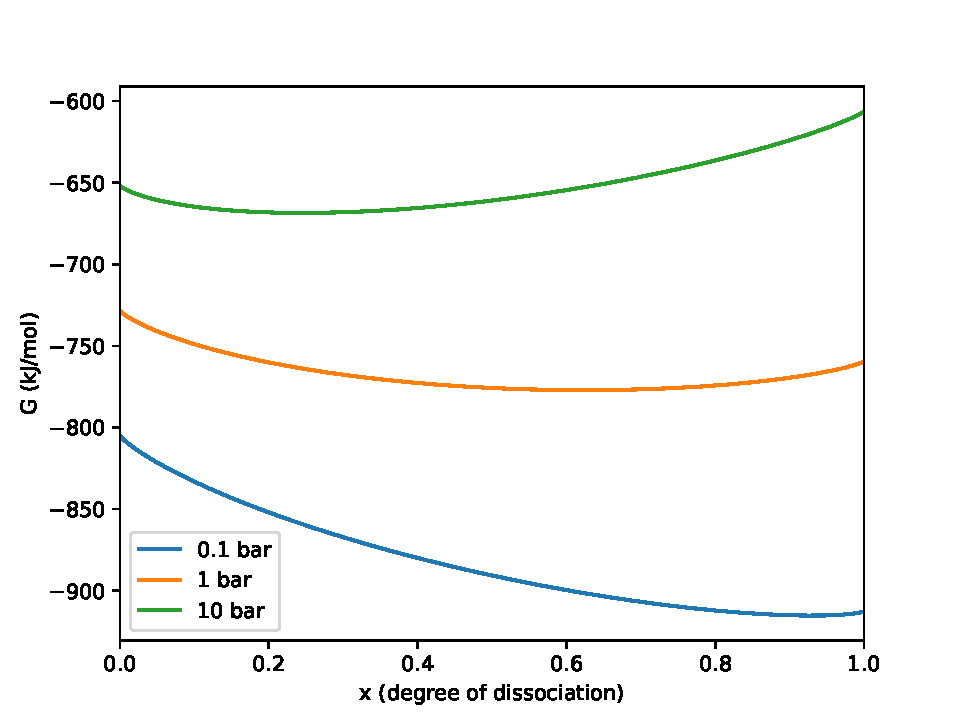
\includegraphics[width=0.7\textwidth]{assets/2 models/Gibbs.pdf}
            \caption{Gibbs free energy (G) plotted against the degree of dissociation (x) of hydrogen under three different pressures}
            \label{fig:Gibbs}
        \end{figure}

        A similar dissociation graph can be found with argon, but with three species. The Gibbs energy is then minimized to determine the molar fractions $y_i$ at which the mixture reaches equilibrium. From this, the enthalpy $H$ of the mixture was found. The $C_p$ of the mixture was then calculated from the enthalpy with:

        \begin{equation}
            C_p = \frac{\partial H}{\partial T}\bigg|_{p = const.}
        \end{equation}
        
        For argon, these calculated $C_p$ values were validated against values from CEA \cite{CEARUNRev4} in \autoref{fig:Cp_compare}.
        
        \begin{figure}[!ht]
            \centering
            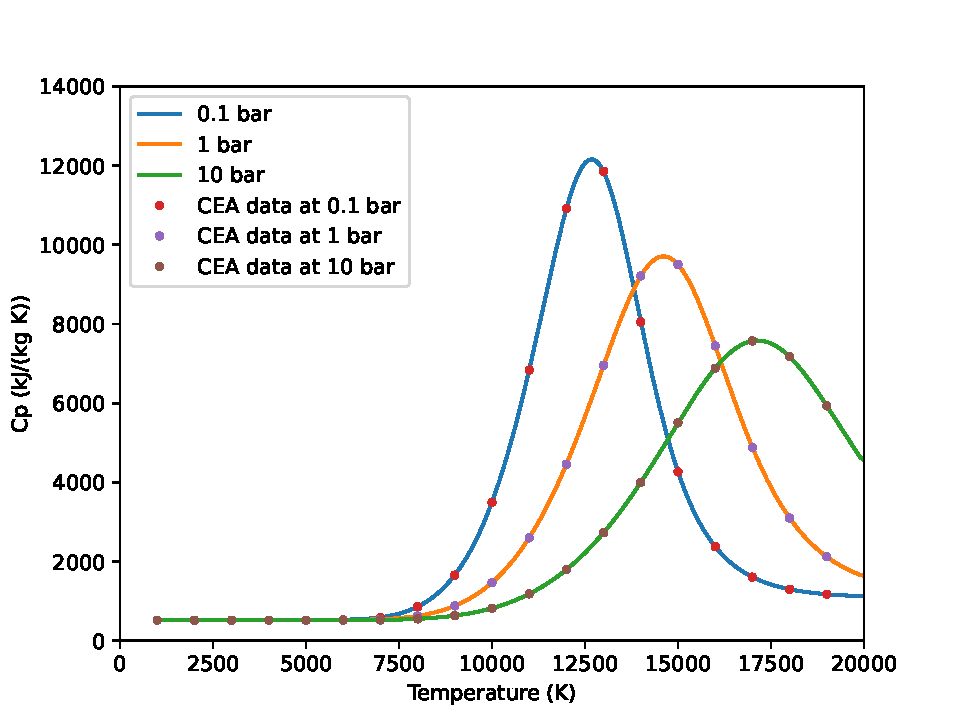
\includegraphics[width=0.7\textwidth]{assets/2 models/Cp_compare.pdf}
            \caption{Comparing calculated $C_p$ values of argon to those from CEA}
            \label{fig:Cp_compare}
        \end{figure}

        The properties of the argon plasma will be used as the basis of the 0D LSP model.
    
    \section{Bremsstrahlung}
        
        The main source of radiation found in LSP is Bremsstrahlung, or braking radiation. When an electron passes close to a heavier ion, it is deflected by the ion's electric field. This elastic collision releases a photon \todo{source}. The total radiated power of the collisions can then be calculated with the formulas presented in \autoref{tab:Brems_compare}.

        \begin{table}[!ht]
            \footnotesize
            \centering
            \caption{Comparison of Bremsstrahlung loss power}
            \label{tab:Brems_compare}
            \begin{tabularx}{\textwidth}{@{}lXX@{}}
            \toprule
            \textbf{Reference} & \textbf{Formula} & \textbf{SI Conversion} \\ \midrule
            \textcite{glasstoneControlledThermonuclearReactions1975}  & $P_\mathrm{br} = 1.57 \times 10^{-27} n_\mathrm{e} n_\mathrm{i} Z^2 T^{1/2}$ \: $\mathrm{ergs/(cm^3\cdot s)}$, with T in K. &   $P_\mathrm{br} = 1.57 \times 10^{-28} n_\mathrm{e} n_\mathrm{i} Z^2 T^{1/2} \: \mathrm{W/m^3}$  \\
            \textcite{rybickiRadiativeProcessesAstrophysics2004}      & $P_\mathrm{br} = 1.4 \times 10^{-27} n_\mathrm{e} n_\mathrm{i} Z^2 T^{1/2} \bar{g}_\mathrm{B}$ \: $\mathrm{ergs/(cm^3\cdot s)}$, with T in K.&  $P_\mathrm{br} = 1.68 \times 10^{-28} n_\mathrm{e} n_\mathrm{i} Z^2 T^{1/2} \: \mathrm{W/m^3}$, using $\bar{g}_\mathrm{B} (T)$ = 1.2\\
            \bottomrule          
            \end{tabularx}
        \end{table}

        The first relation, from \textcite{glasstoneControlledThermonuclearReactions1975} converted to SI, was used for the remainder of the calculations.

        There is also a question regarding whether the plasma is a surface emitter or a volume emitter. This is determined by calculating the plasma frequency at a typical electron density and comparing it to the wavelength of the light emitted by Bremsstrahlung. If the plasma frequency is higher than the wavelength of emitted Bremsstrahlung light, then it is cut off by the plasma; no light can escape the volume of the LSP cone, and it is a surface emitter. If it is lower, then the emitted photons are not blocked by the LSP and the cone is a volumetric emitter.
        
        The plasma frequency $\omega_\mathrm{p}$ is found with: 

        \begin{equation}
            \omega_\mathrm{p} = \sqrt{\frac{n_\mathrm{e} e^2}{\epsilon_\mathrm{0} m_\mathrm{e}}}
        \end{equation}

        With $n_\mathrm{e}$ the plasma electron density, $e$ the elementary charge, $\epsilon_\mathrm{0}$ the vacuum permittivity and $m_\mathrm{e}$ the electron mass.

        At \todo{todo} XX K and \todo{todo} XX Pa, an electron density of \todo{todo} XX is found. This results in $\omega_p =$ \qty{3.10e12}{Hz}. Considering visible light and above (> \qty{1e14}{Hz}) as the wavelengths of interest, the LSP is indeed a volume emitter.

    \section{Model setup}
        
        Finally, a simple 0D model was written in Python to attempt to explain the pressure rise seen in the LTP experiments. \autoref{fig:0D model} illustrates this model. Laser energy is focused into a volume of argon, creating an LSP cone. Energy is transferred from the LSP cone to the larger argon volume by Bremsstrahlung\todo{Have the arrow go from cone to volume, not outside!}. \todo{A part of the laser energy is also transmitted through the cone to the outside of the argon volume and lost.} The LSP is treated as an ideal gas.

        \begin{figure}[!ht]
            \centering
            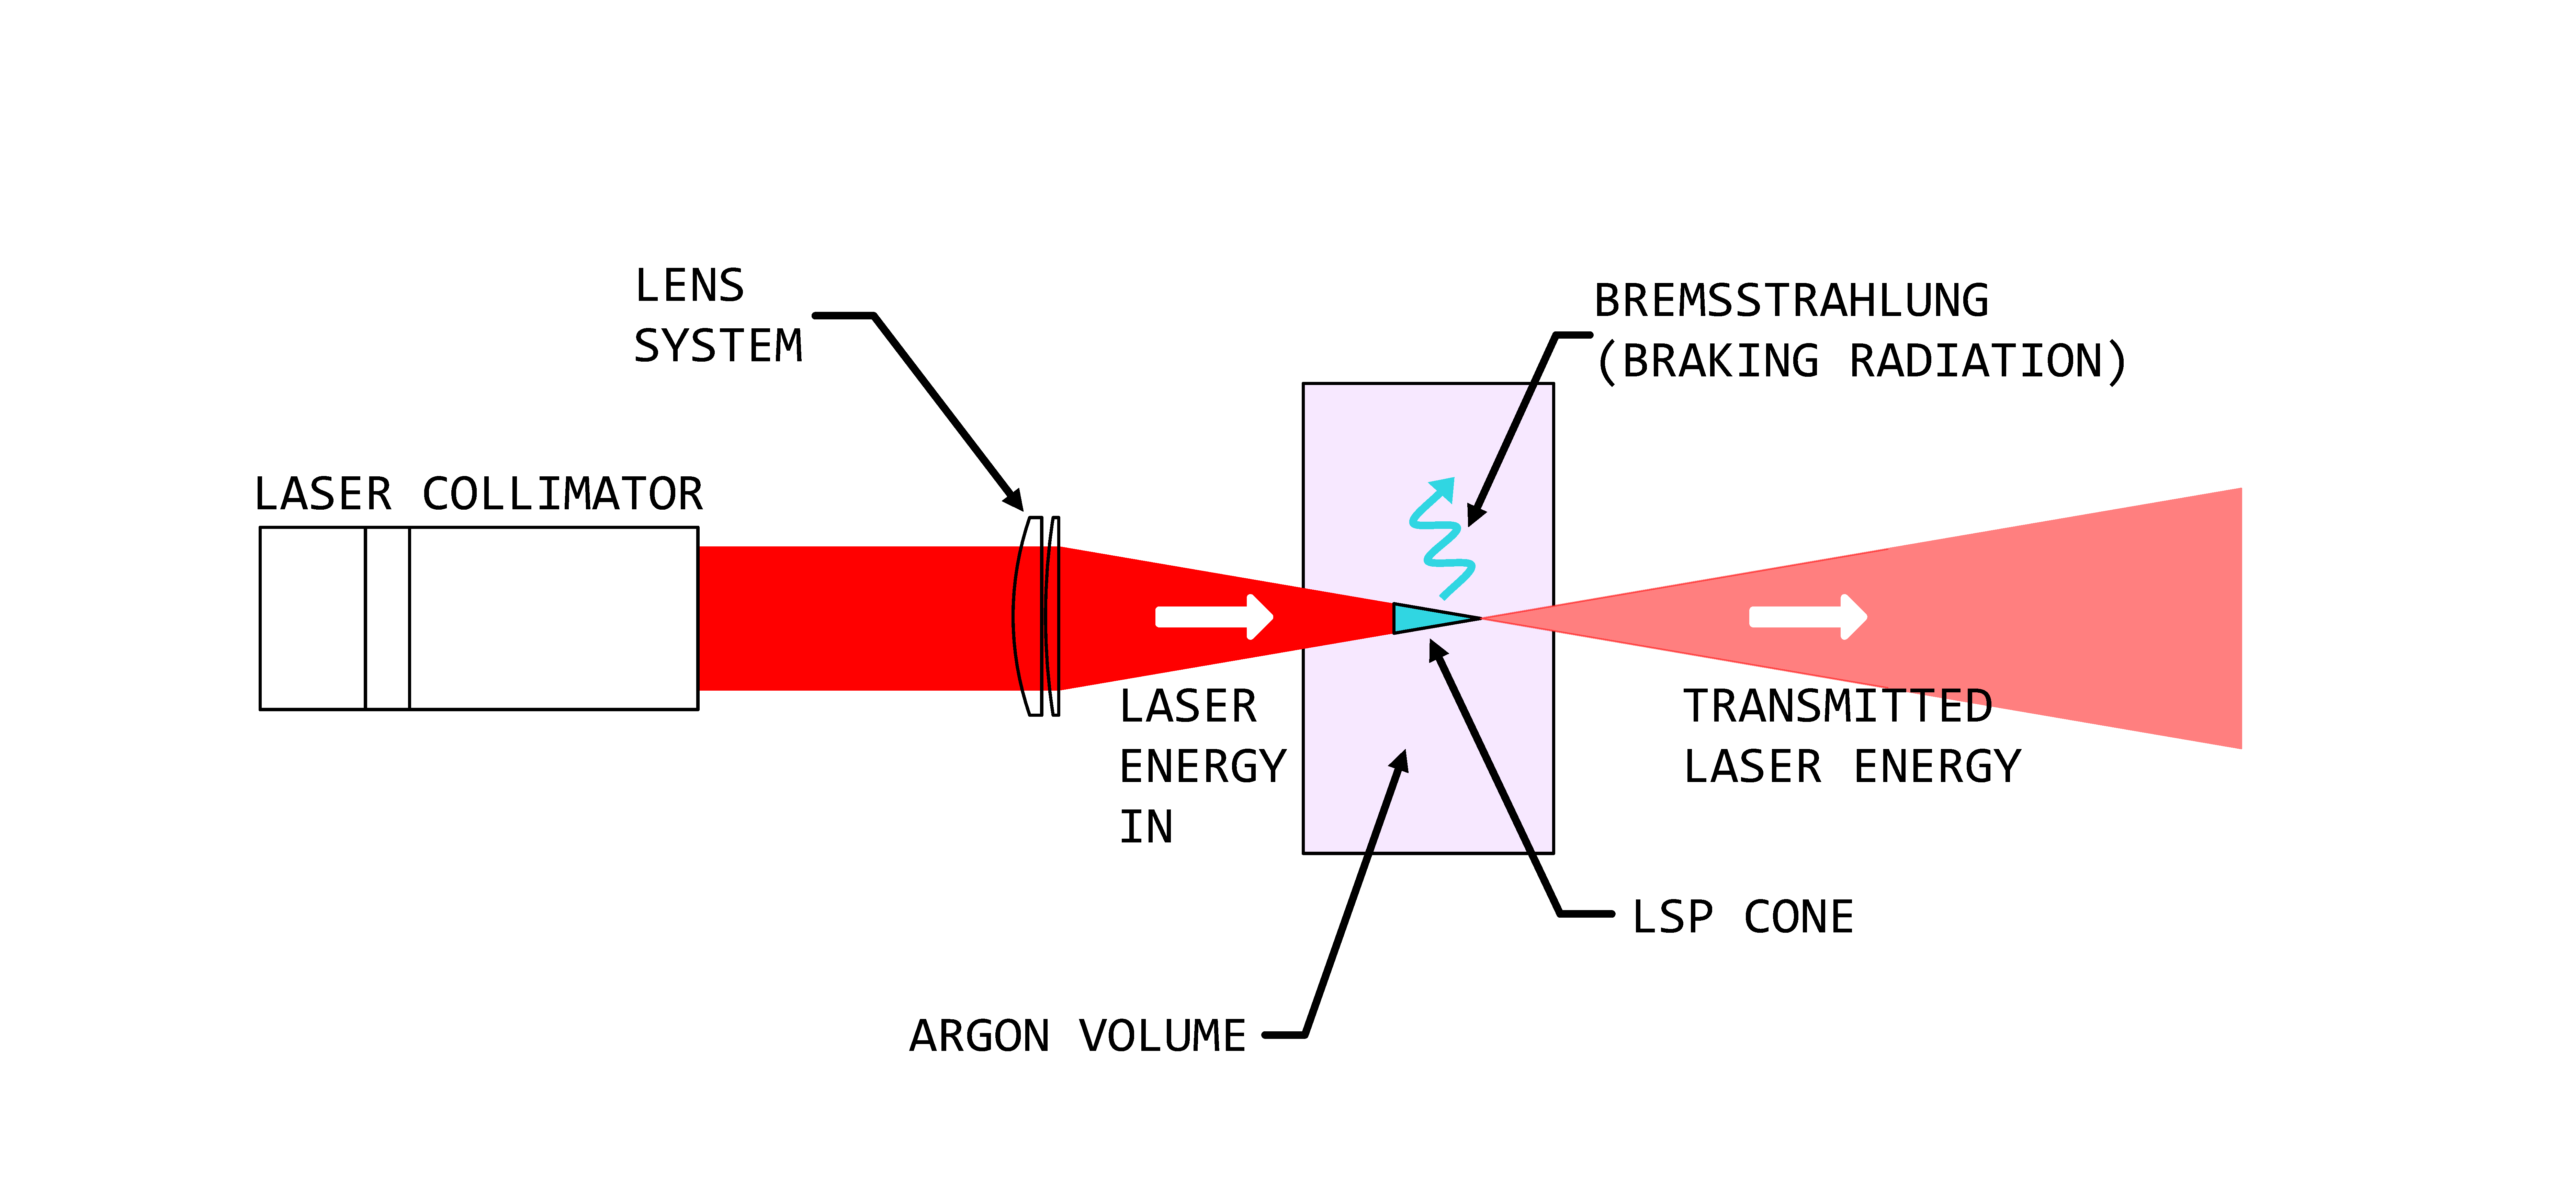
\includegraphics[width=0.85\textwidth]{assets/2 models/Modeling figure.pdf}
            \caption{0D model of an LSP inside a volume of pressurized argon}
            \label{fig:0D model}
        \end{figure}

        The calculation procedure that was implemented is as follows:

        \begin{enumerate}
            \item The volume and the mass of a cone of pure argon is found at the initial temperature (\qty{300}{K}) and pressure (\qty{20}{bar}). This mass will remain fixed for the rest of the problem
                \begin{equation}
                    huh
                \end{equation}
            \item Energy from the laser pulse is added to the cone at constant pressure and the new temperature at this step is found ($T_2$)
                \begin{equation}
                    E_\mathrm{plasma} = E_\mathrm{plasma} + P_\mathrm{laser} \times \mathrm{timestep} - P_\mathrm{loss} \times \mathrm{timestep}
                \end{equation}
                \begin{equation}
                    m_{plasma} (h_2 - h_1) = E_{laser}
                \end{equation}
                Where this equation is solved for 
            \item The number of moles in the LSP are found by minimizing the Gibbs free energy at the temperature and pressure of step 2. The new volume of the cone ($V_2$) is then found with the ideal gas law.
            \item The pressure increase in the chamber due to the isentropic expansion of the gas in the LSP cone is calculated ($p_4$)
                \begin{equation}
                    p_4 = p_\mathrm{ini} ((V_\mathrm{chamber} - V_\mathrm{plasma})/(V_\mathrm{chamber} - V_2))^k
                \end{equation}
            \item The radiated power from the LSP cone to the larger argon volume is determined using the Bremsstrahlung total power loss equation from \textcite{glasstoneControlledThermonuclearReactions1975}.
                \begin{equation}
                    P_\mathrm{br} = 1.57 \times 10^{-28} n_\mathrm{e} n_\mathrm{i} Z^2 T^{1/2}
                \end{equation}
            \item Steps 2 to 5 are looped until \qty{10}{ms}, when the laser shuts off. No more energy is added but Bremsstrahlung loss continues. The conservation of energy equation then becomes:
                \begin{equation}
                    E_\mathrm{plasma} = E_\mathrm{plasma} - P_\mathrm{loss} \times \mathrm{timestep}
                \end{equation}
        \end{enumerate}
        
        To determine an upper bound on power loss, a switch was implemented to change Bremsstrahlung loss to blackbody radiation loss.

    \section{Model results}

        \begin{figure}[!ht]
            \centering
            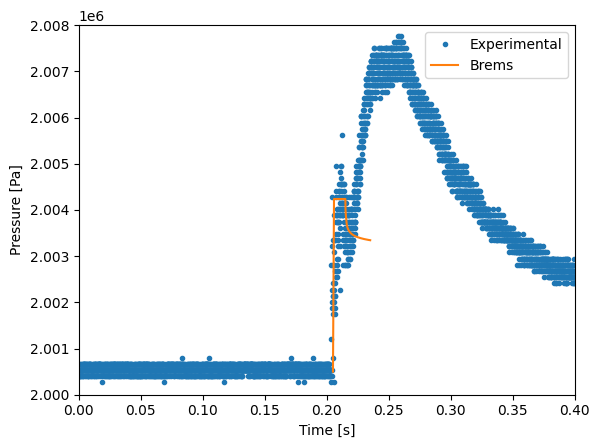
\includegraphics[width=0.85\textwidth]{assets/2 models/Brems vs exp graph.png}
            \caption{Experimental data compared to the 0D model, with both Bremsstrahlung and blackbody losses}
            \label{fig:Model results}
        \end{figure}

        \todo{Add blackbody radiation loss, add laser pulse "on" area.} From these iterations, \autoref{fig:Model results} was drawn. Using Bremsstrahlung loss, the model appropriately approximates the first peak seen in the experimental data. Once the gas cools down enough and stops being ionized, Bremsstrahlung loss stops. The LSP cone in the model is then stable at approximately a temperature of \qty{5200}{K} and a pressure of \qty{2.003}{MPa}. The second peak could be explained by the fact that the energy in the cone is then communicated to the rest of the argon volume, equalizing temperatures and pressures.
    \chapter{Facility design}

    \section{Version 1 test section} \label{sec:design_v1}

        The design process of the first generation thruster, called Version 1 (V1), can be found in \textcite{duplayArgonLaserPlasmaThruster2024a}. It proved to be a dependable prototype, repurposed from a previous unrelated experiment. However, it presented problems that required a second generation prototype to be designed and manufactured.

        \begin{figure}[!ht]
            \centering
            \begin{subfigure}[t]{\textwidth}
                \includegraphics[width=0.85\textwidth]{assets/3 design/finalsetup_static.pdf}
                \caption{Static setup}
            \end{subfigure}
            \hfill
            \begin{subfigure}[t]{\textwidth}
                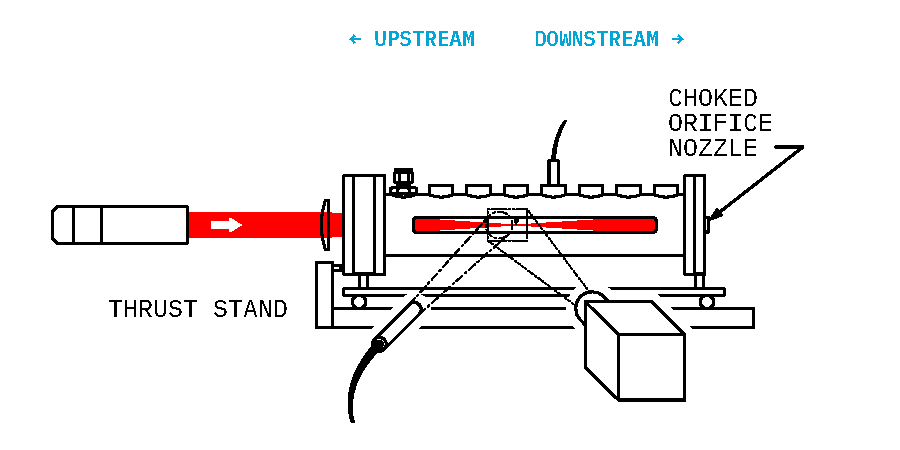
\includegraphics[width=0.85\textwidth]{assets/3 design/finalsetup_flowing.pdf}
                \caption{Flowing setup}
            \end{subfigure}
            \caption{V1 LTP thruster}
            \label{fig:V1 setup}
        \end{figure}

        298 recorded pulsed laser shots were conducted with V1, exploring the power-pressure threshold, wire initiation and spark initiation. A side window permitted direct visualization of the LSP with a high speed camera (Photron Fastcam SA5).

        % Adding holes on bottom for wire ignition

        However, this test section was made of steel, creating too much friction on its rails during thrust tests. This was mitigated in part by a rope system mentioned in \textcite{duplayArgonLaserPlasmaThruster2024a}, but was not found to be repeatable. Having the LSP heat a smaller internal volume than the \qty{0.4}{L} of V1 was also desirable, as a greater effect on internal pressure and thrust would be seen.

        Critically, rubber seals were exposed to the laser path during continuous (CW) lasing with a lower focal length lens (picture), severely burning them in the only CW test conducted. A shorter test section designed for a \qty{100}{mm} focal length lens would solve this.

    \section{Version 2} \label{sec:design_v2}

        To improve upon the V1 facility, an entire LTP thruster redesign was done. This resulted in the much smaller Version 2 (V2) purpose-built LTP thruster at the end of April 2024.

        \subsection{Requirements}

            The following requirements were developed for the design of the V2 thruster. The objective was to detect a measurable difference in thrust between an argon cold gas thruster and an argon “hot gas” thruster, heated by a laser supported plasma (LSP).

            \begin{enumerate}
                \item Laser thruster
                \begin{enumerate}
                    \item A \qty{300}{W} Continuous Wave (CW) \qty{1070}{nm} laser shall sustain the plasma (Nominal power \qty{300}{W}, actual max power \qty{350}{W})
                    \item The thruster shall have a minimum safe “hot” operation time of \qty{30}{s}
                    \begin{enumerate}
                        \item In the event of failed LSP initiation, the thruster shall safely absorb the total laser power for at least \qty{10}{s}
                    \end{enumerate}
                    \item An optical path shall be present to let the laser into the thruster, utilizing a \qty{100}{mm} focal length lens at minimum and a collimated beam with a maximum diameter of \qty{30}{mm}
                    \begin{enumerate}
                        \item The optical components shall not be damaged by the laser flux
                    \end{enumerate}
                    \item Argon shall be used as the working fluid
                    \begin{enumerate}
                        \item The argon feed gas shall be at room temperature
                    \end{enumerate}
                    \item A gas feed path shall bring argon gas into the thruster
                    \begin{enumerate}
                        \item The gas feed shall be choked at the thruster inlet
                        \item The gas feed shall be evenly distributed in the thruster
                    \end{enumerate}
                    \item The mass flow rate of the argon gas shall be measured and controlled by interchangeable upstream choked orifices
                    \item The maximum allowable operating pressure (MAOP) of the thruster shall be 50 bar
                    \begin{enumerate}
                        \item The nominal pressure of the thruster shall be 25 bar
                    \end{enumerate}
                    \item A converging-diverging exhaust nozzle shall be designed to accelerate the gas to a supersonic speed
                    \begin{enumerate}
                        \item The nozzle shall be easily changeable
                    \end{enumerate}
                    \item A 1/8" NPT port for a pressure transducer shall be present along the thruster
                    \item An optical port shall be present for spectrometry measurements of the plasma
                    \item The thruster shall be installed on a thrust stand (See section 3. Thrust stand)
                \end{enumerate}
                \item Initiation system/electrical
                \begin{enumerate}
                    \item The LSP shall be ignited by an electrical spark
                    \item The spark gap shall be measurable, controllable, and repeatable
                    \item The spark shall be generated by an AEM 30-2853 High Output Smart Coil, supplying \qty{41}{kV} with up to \qty{118}{mJ}
                    \item All parts of the thruster and thrust stand shall be directly or indirectly connected to a common electrical ground
                \end{enumerate}
                \item Thrust stand
                \begin{enumerate}
                    \item The thrust stand shall measure thrust on the order of \qtyrange{0.1}{5}{N}
                    \item The thrust stand shall minimize friction losses
                    \item The thrust stand shall be securely fixed using standard optical breadboard mounting hardware
                \end{enumerate}
            \end{enumerate}

            With these requirements, preliminary geometric dimensions of the V2 thruster could commence. It was expected to be much smaller than V1, as the goal was to isolate the LSP region and increase heat flux to the gas.
        
        \subsection{Test section and thrust stand}

            \begin{figure}[!ht]
                \centering
                \begin{subfigure}[t]{0.45\textwidth}
                    \centering
                    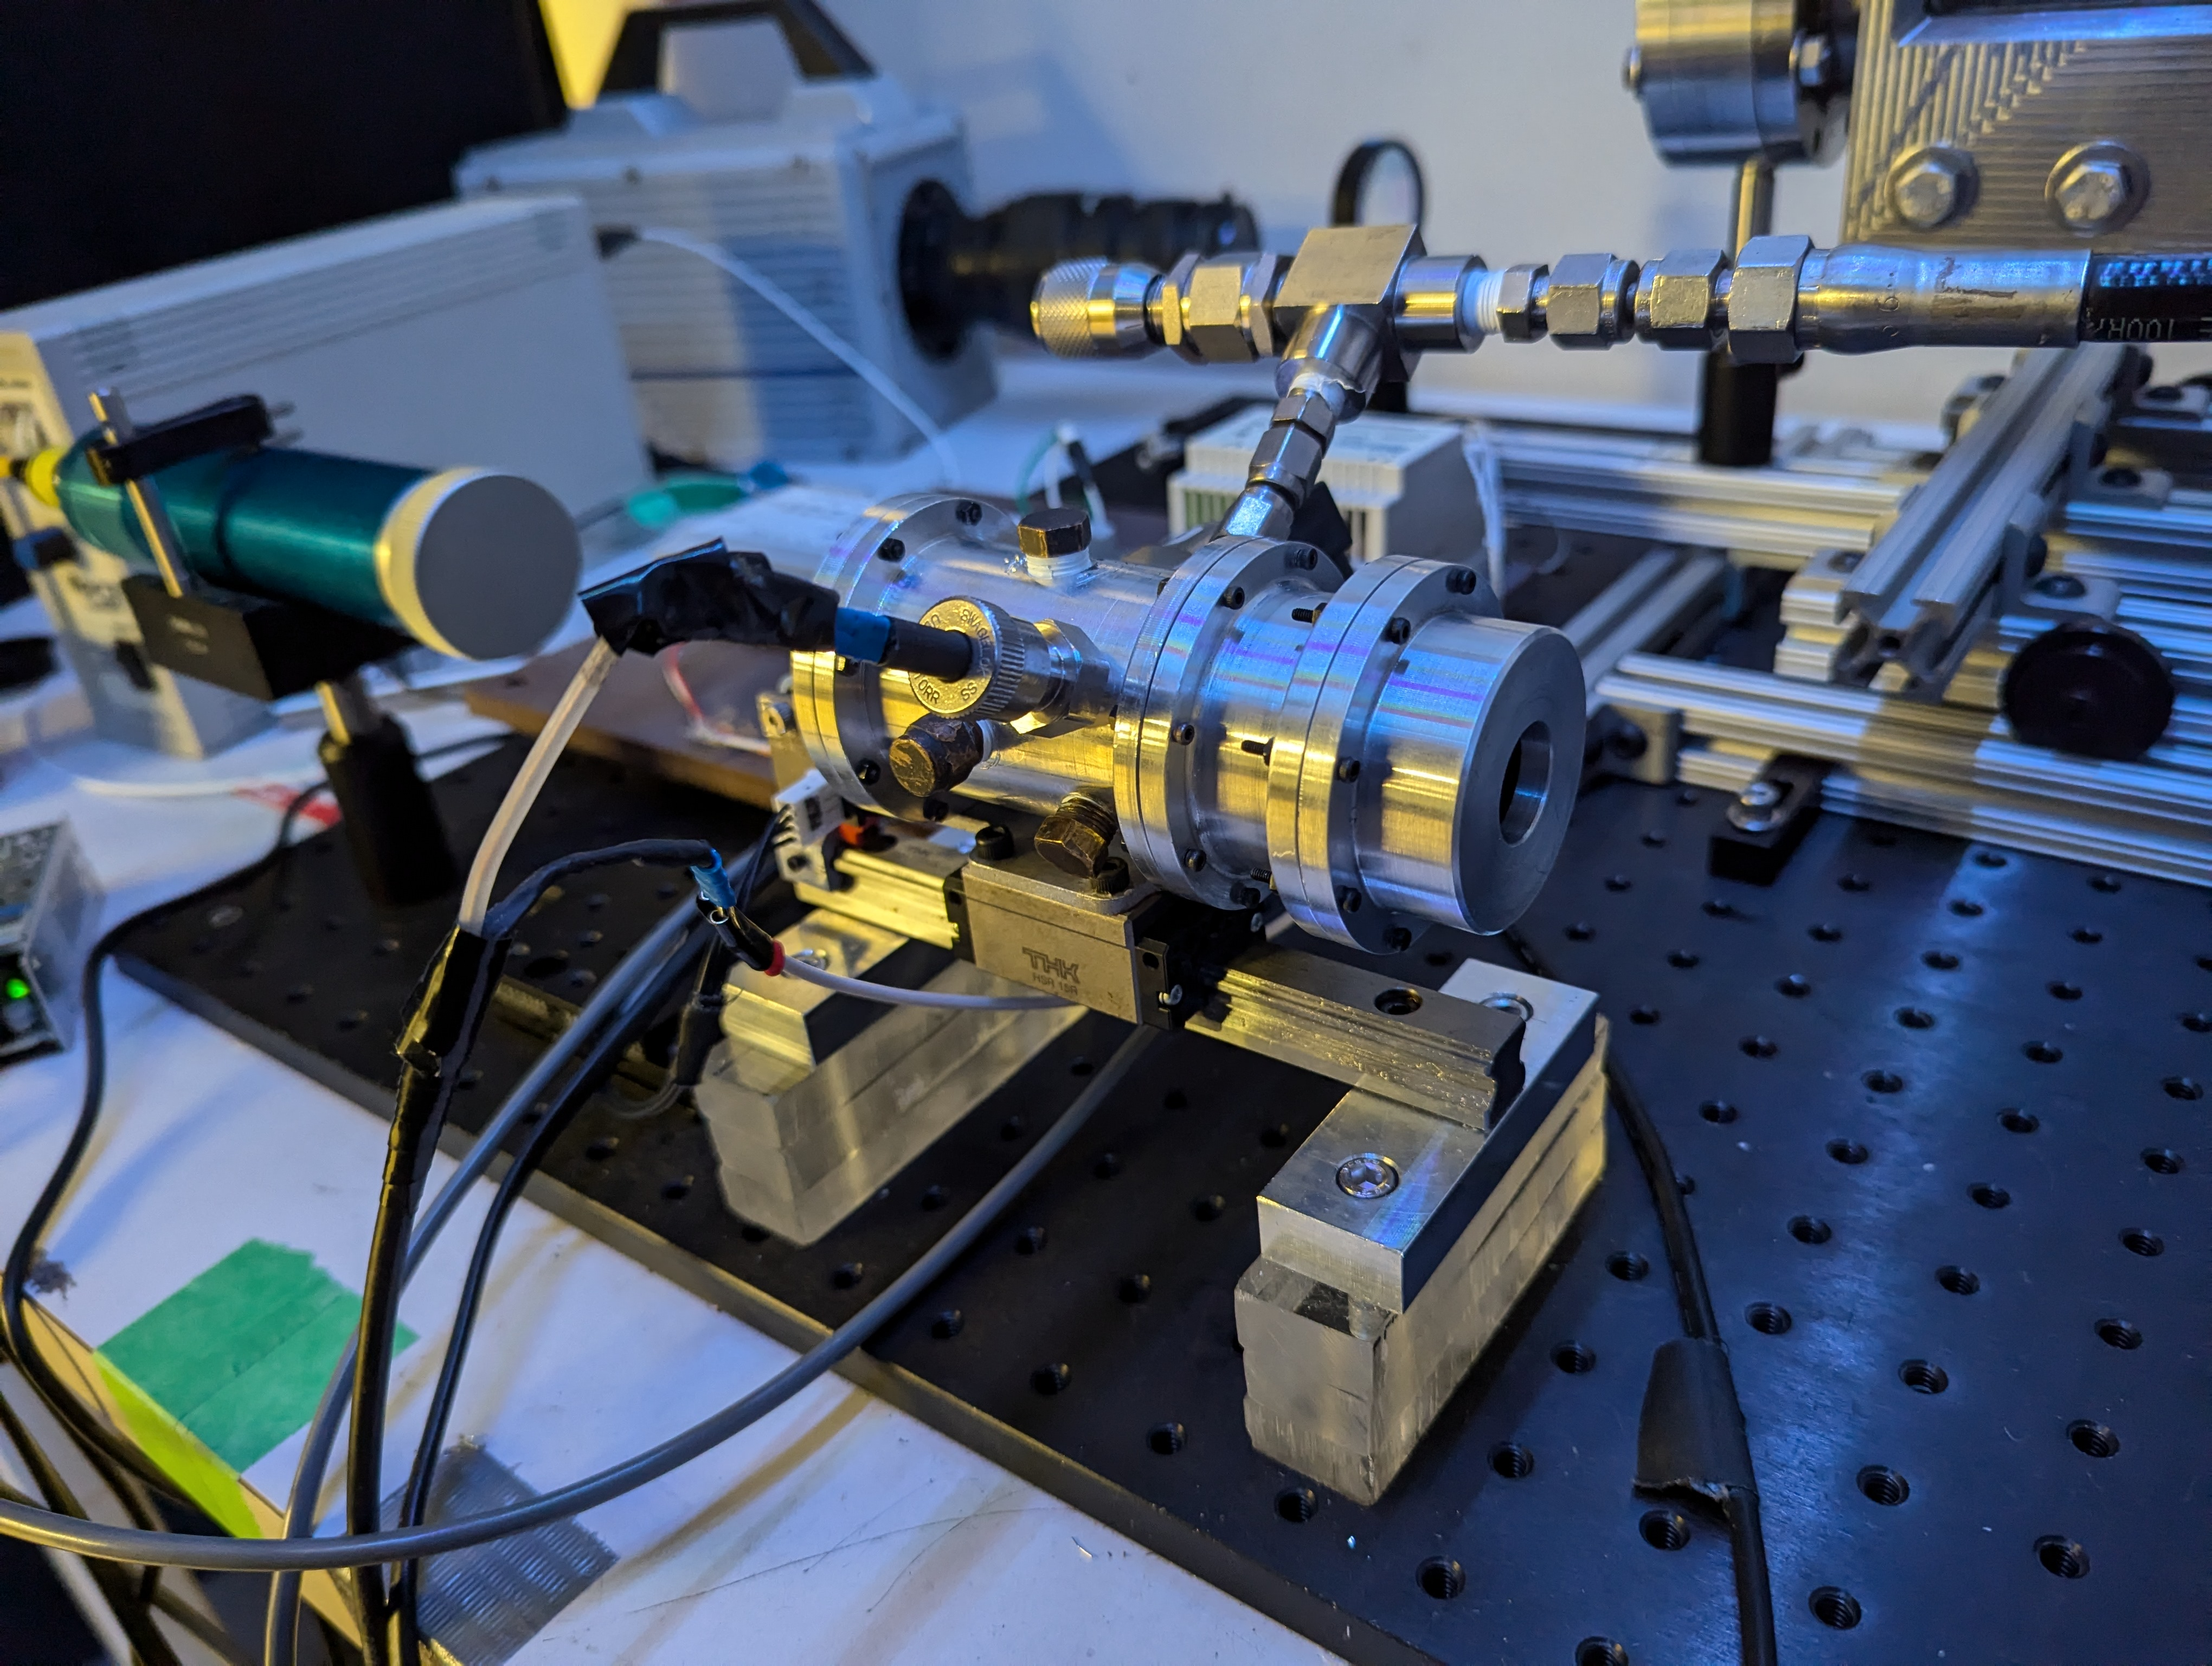
\includegraphics[width=\textwidth]{assets/3 design/V2 Static configuration.jpg}
                    \caption{Static configuration. Note the extension part and window mount.}
                \end{subfigure}
                \hfill
                \begin{subfigure}[t]{0.45\textwidth}
                    \centering
                    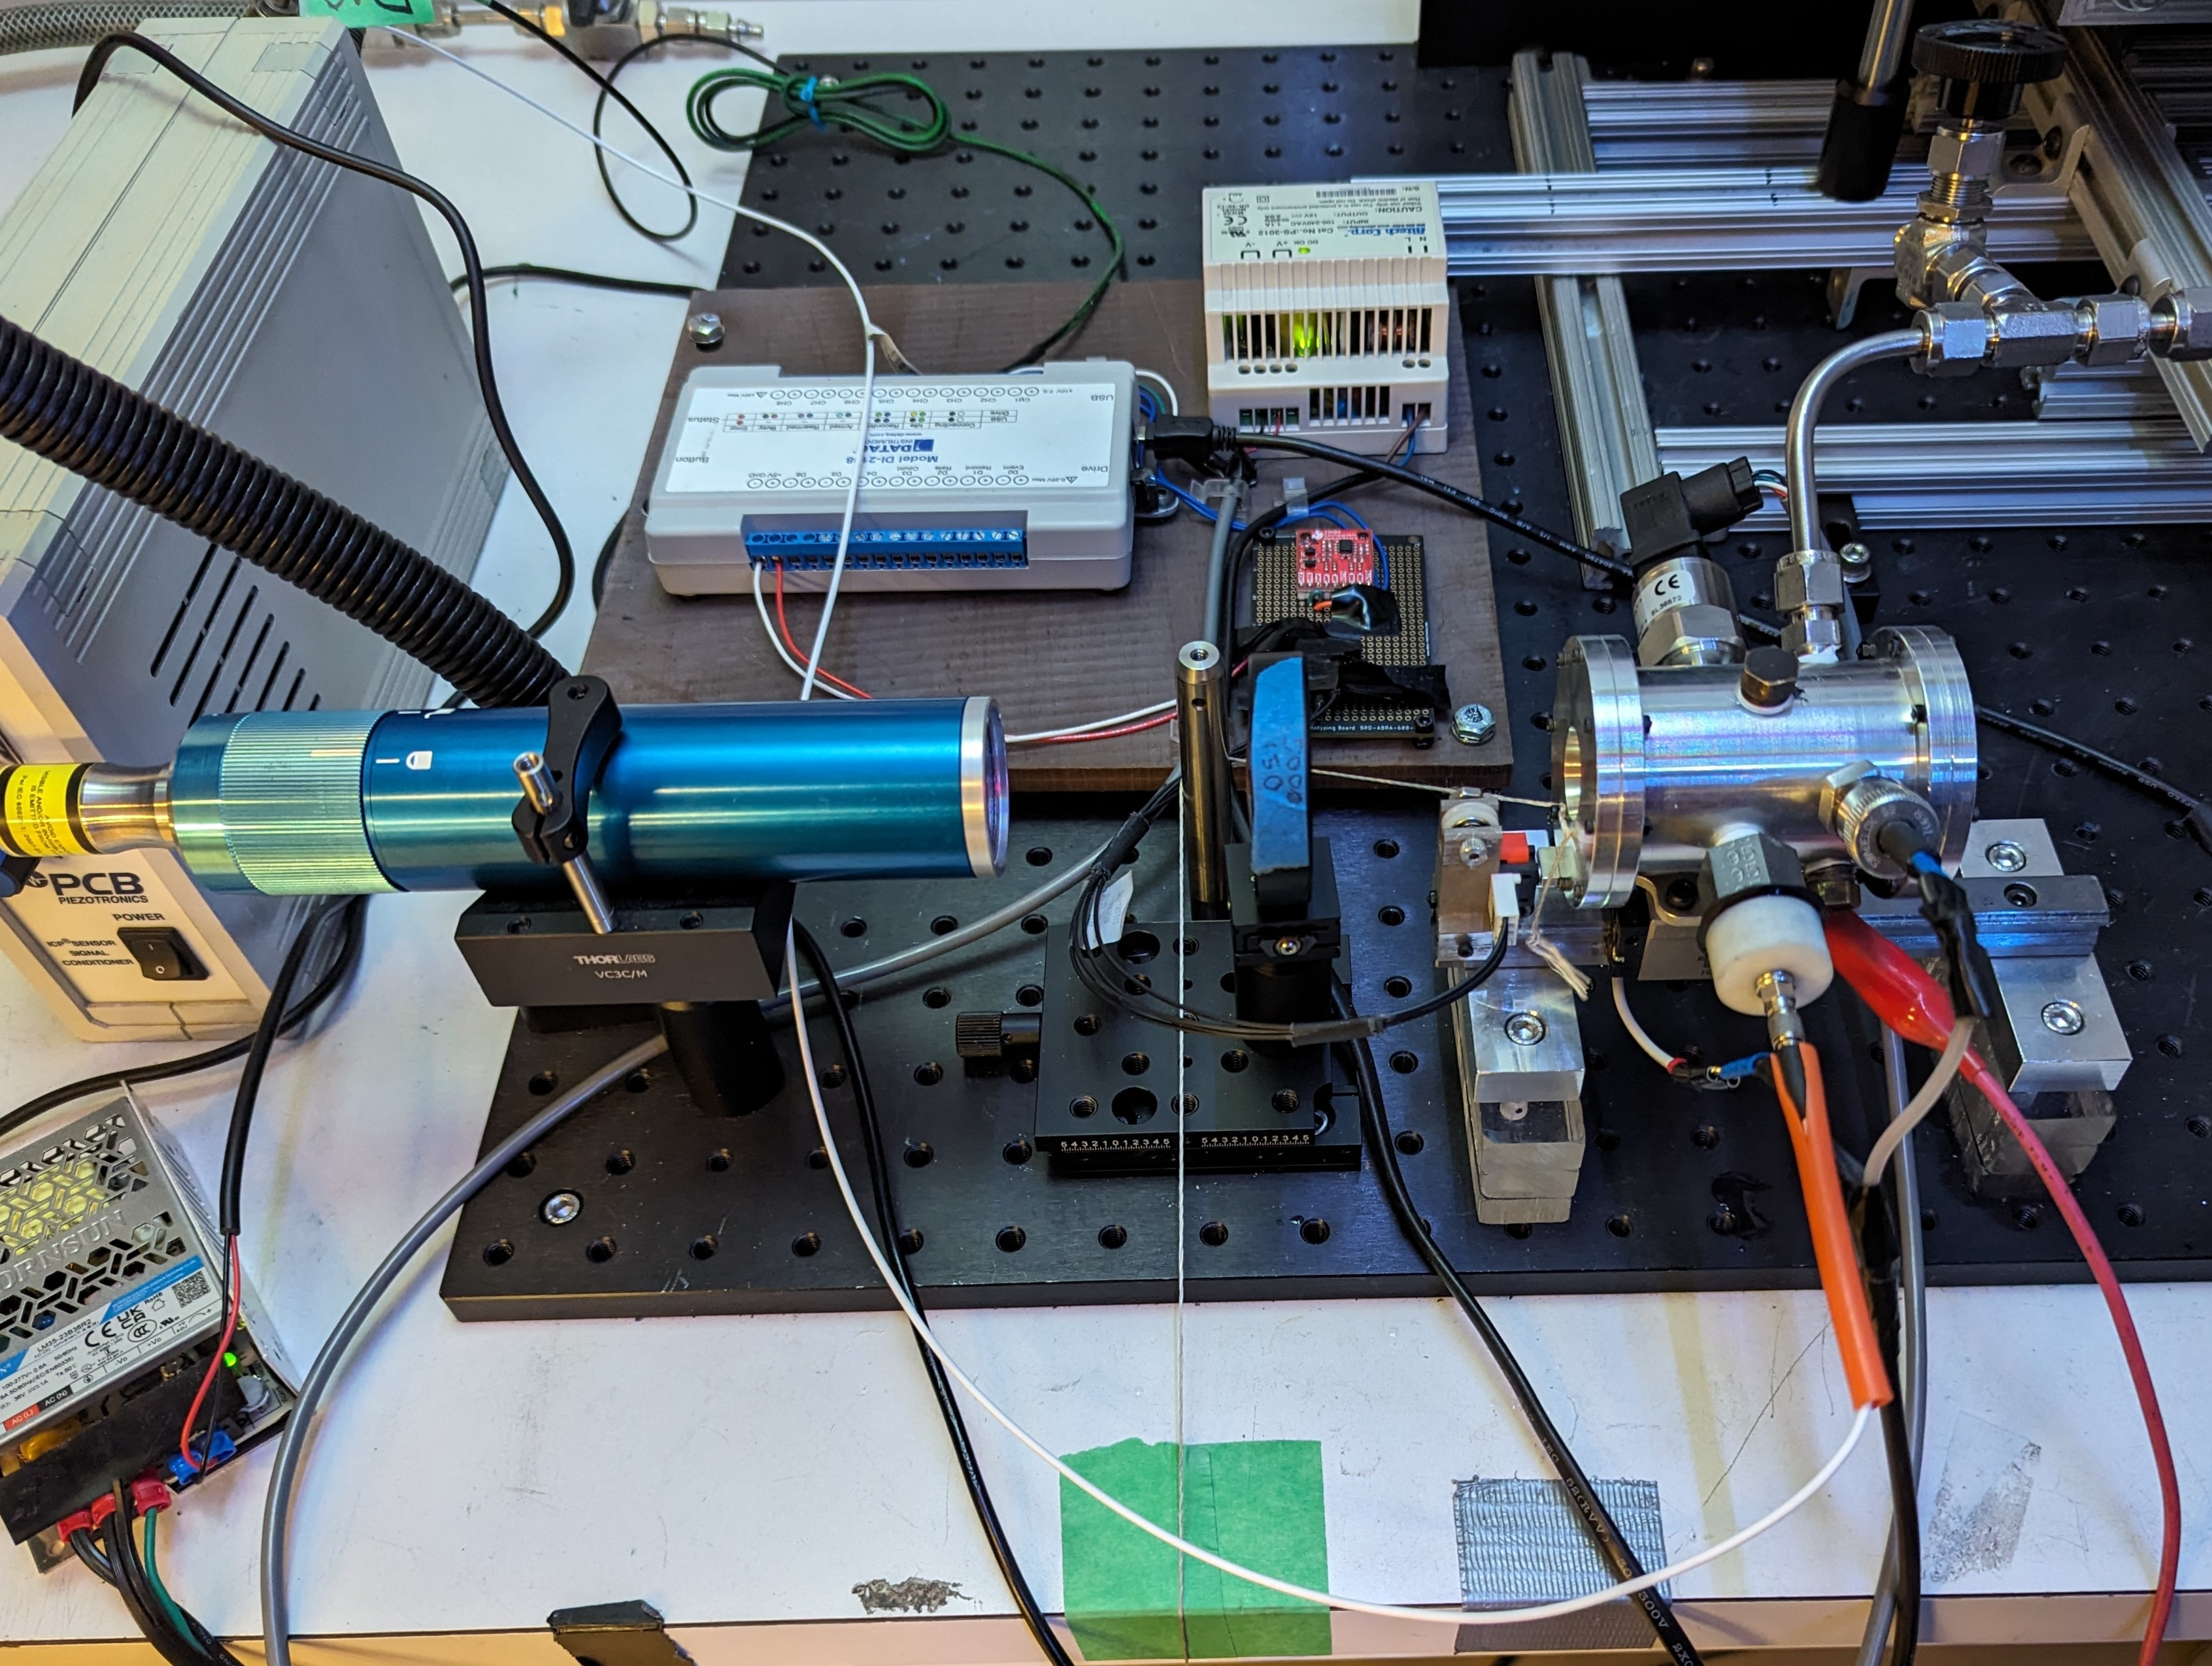
\includegraphics[width=\textwidth]{assets/3 design/V2 flowing setup.jpg}
                    \caption{Flowing configuration. The nozzle is held by the rear plate.}
                \end{subfigure}
                \caption{V2 LTP thruster}
                \label{fig:V2 setup}
            \end{figure}

            The thrust stand is a ball bearing carriage (McMaster-Carr 6709K12) mounted on a \qty{15}{mm} wide rail (McMaster-Carr 6709K33). A string through a pulley holds a variable weight, adding a preload to the test section. This ensures adequate contact between the test section and the load cell. Two load cells are used with different force sensing range: Honeywell FSG020WNPB (\qtyrange{0}{20}{N}) and Honeywell FSG005WNPB (\qtyrange{0}{5}{N}).

        \subsection{Laser}

            The laser used as the plasma's power source is an IPG Photonics YLR-300/3000-QCW-MM-AC Ytterbium fiber laser. The wavelength of the emitted light is \qty{1070}{nm}. Its nominal maximum power is \qty{3}{kW} quasi-continuous wave (QCW) or \qty{300}{W} continuous wave (CW). At \qty{3}{kW}, a QCW pulse has a maximum duration of \qty{10}{ms}. The maximum duration of a \qty{300}{W} QCW pulse is \qty{50}{ms} The laser light exits through an IPG Photonics P30-001736 collimator. The output beam is \qty{30}{mm} in diameter.

            \begin{figure}[!ht]
                \centering
                \begin{subfigure}[t]{0.45\textwidth}
                    \centering
                    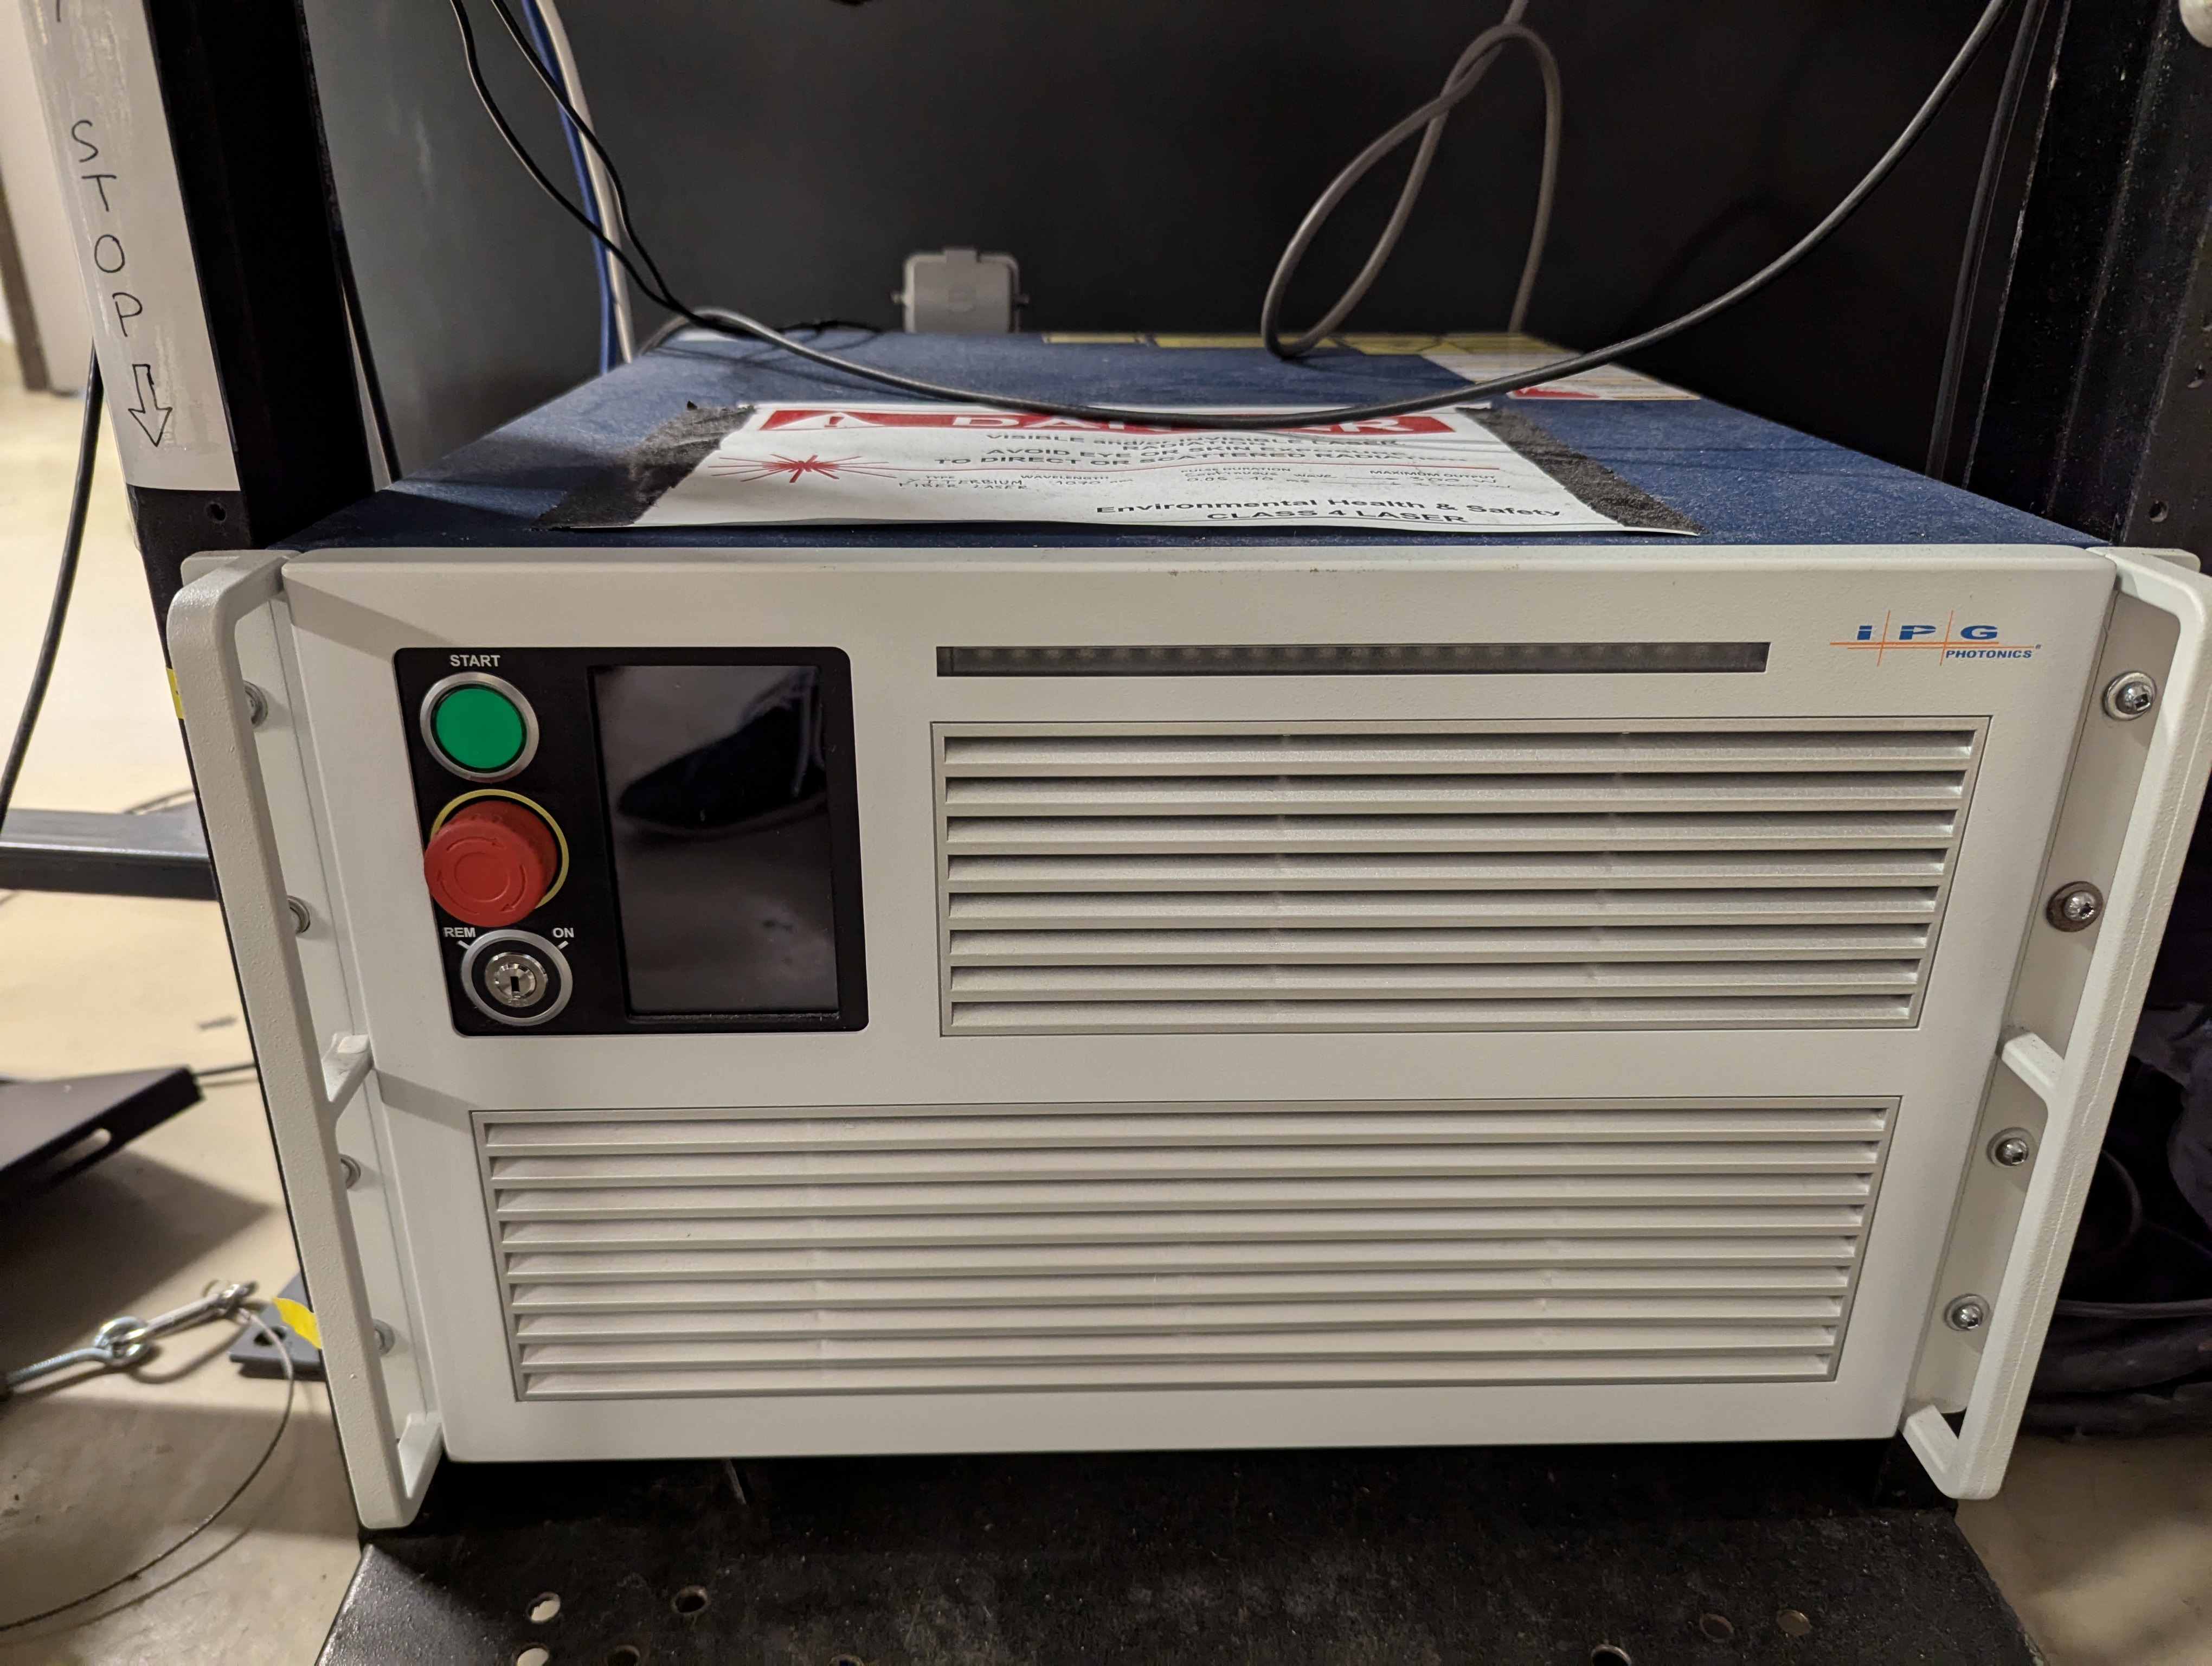
\includegraphics[width=\textwidth]{assets/3 design/Laser box.jpg}
                    \caption{IPG Photonics YLR-300/3000-QCW-MM-AC laser}
                \end{subfigure}
                \hfill
                \begin{subfigure}[t]{0.45\textwidth}
                    \centering
                    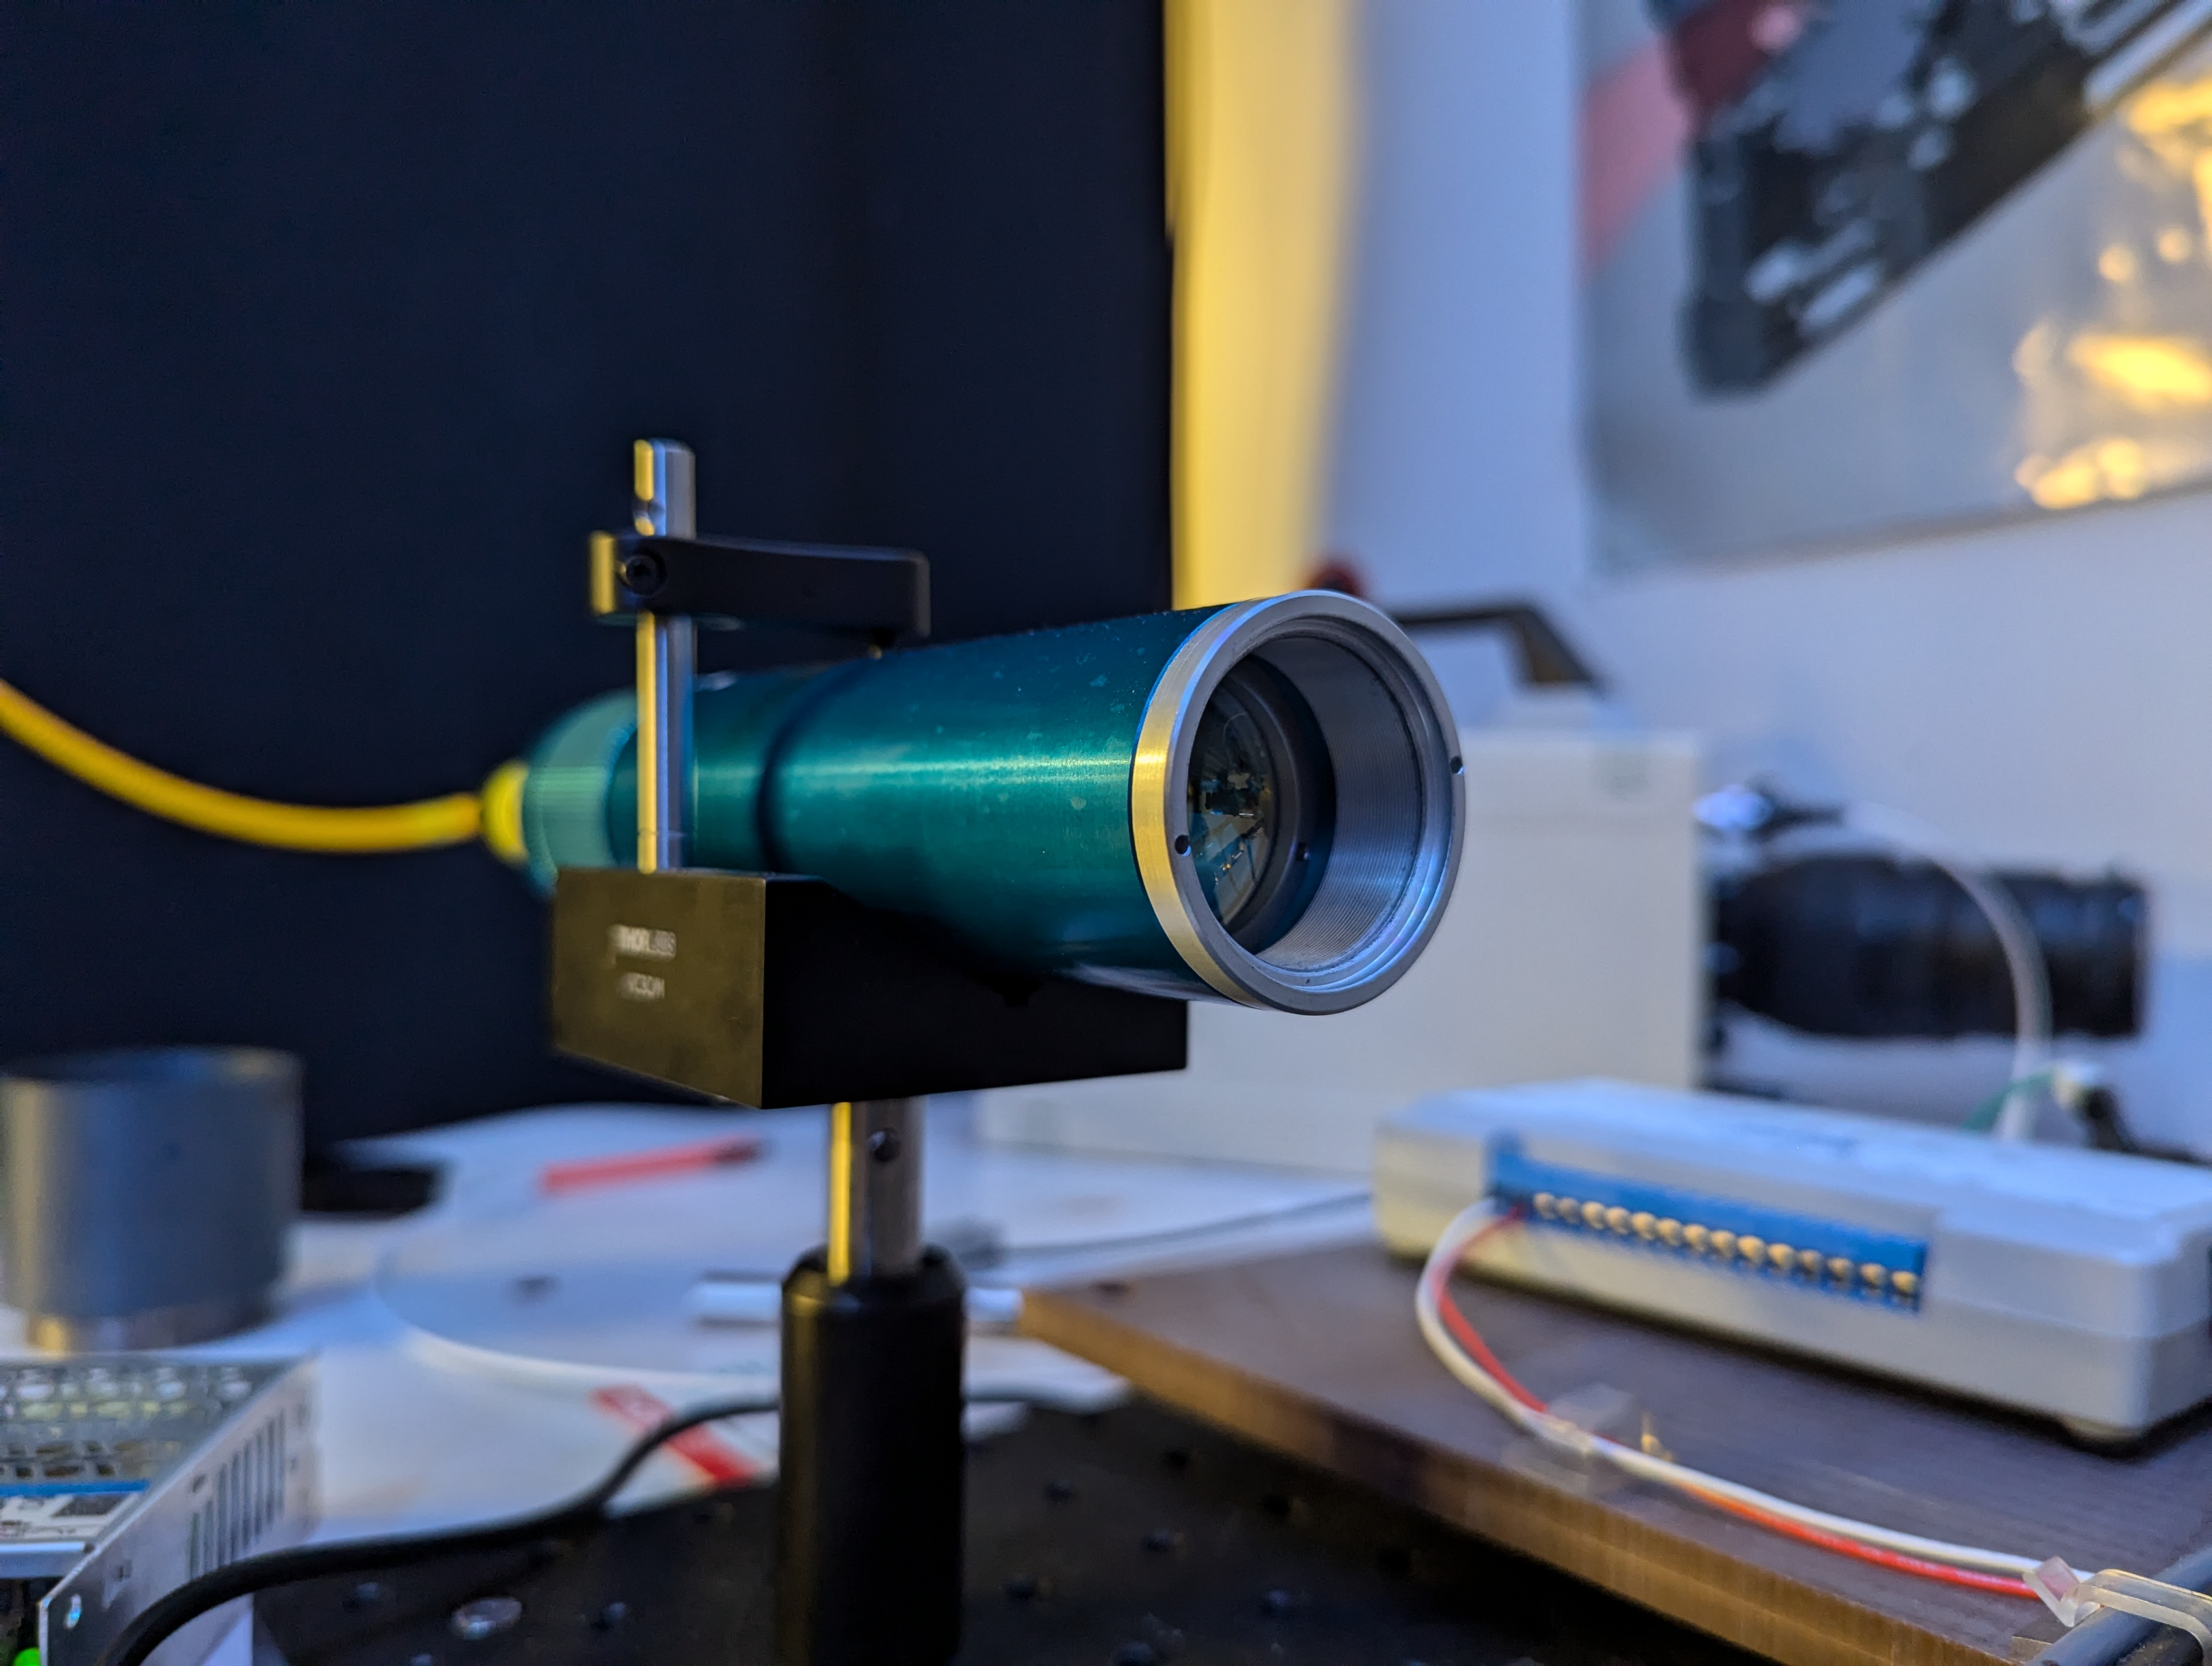
\includegraphics[width=\textwidth]{assets/3 design/Laser aperture.jpg}
                    \caption{IPG Photonics P30-001736 collimator}
                \end{subfigure}
                \caption{Laser system}
            \end{figure}

            Calibration reports for the laser and the collimator can be found in the appendix. [ADD TO APPENDIX]

        \subsection{Spark initiation system}

            AEM coil and electronics box.

        \subsection{Timing control}

            Correct timing of the laser and spark initiation is necessary to initiate LSP when the laser is in QCW mode, and to minimize damage to V2's nozzle in CW mode. To this end, delay generators are used (BNC models 7010 and 7055).

        \subsection{Data acquisition (DAQ) system and oscilloscope}

            Load cell and pressure transducer voltage is sent to a DATAQ Instruments DI-2018. This data is streamed to a personal computer by USB, where the thrust and pressure traces can be saved for analysis. Two pressure sensors were used: [PCB and OMEGA]

            \begin{figure}[!ht]
                \centering
                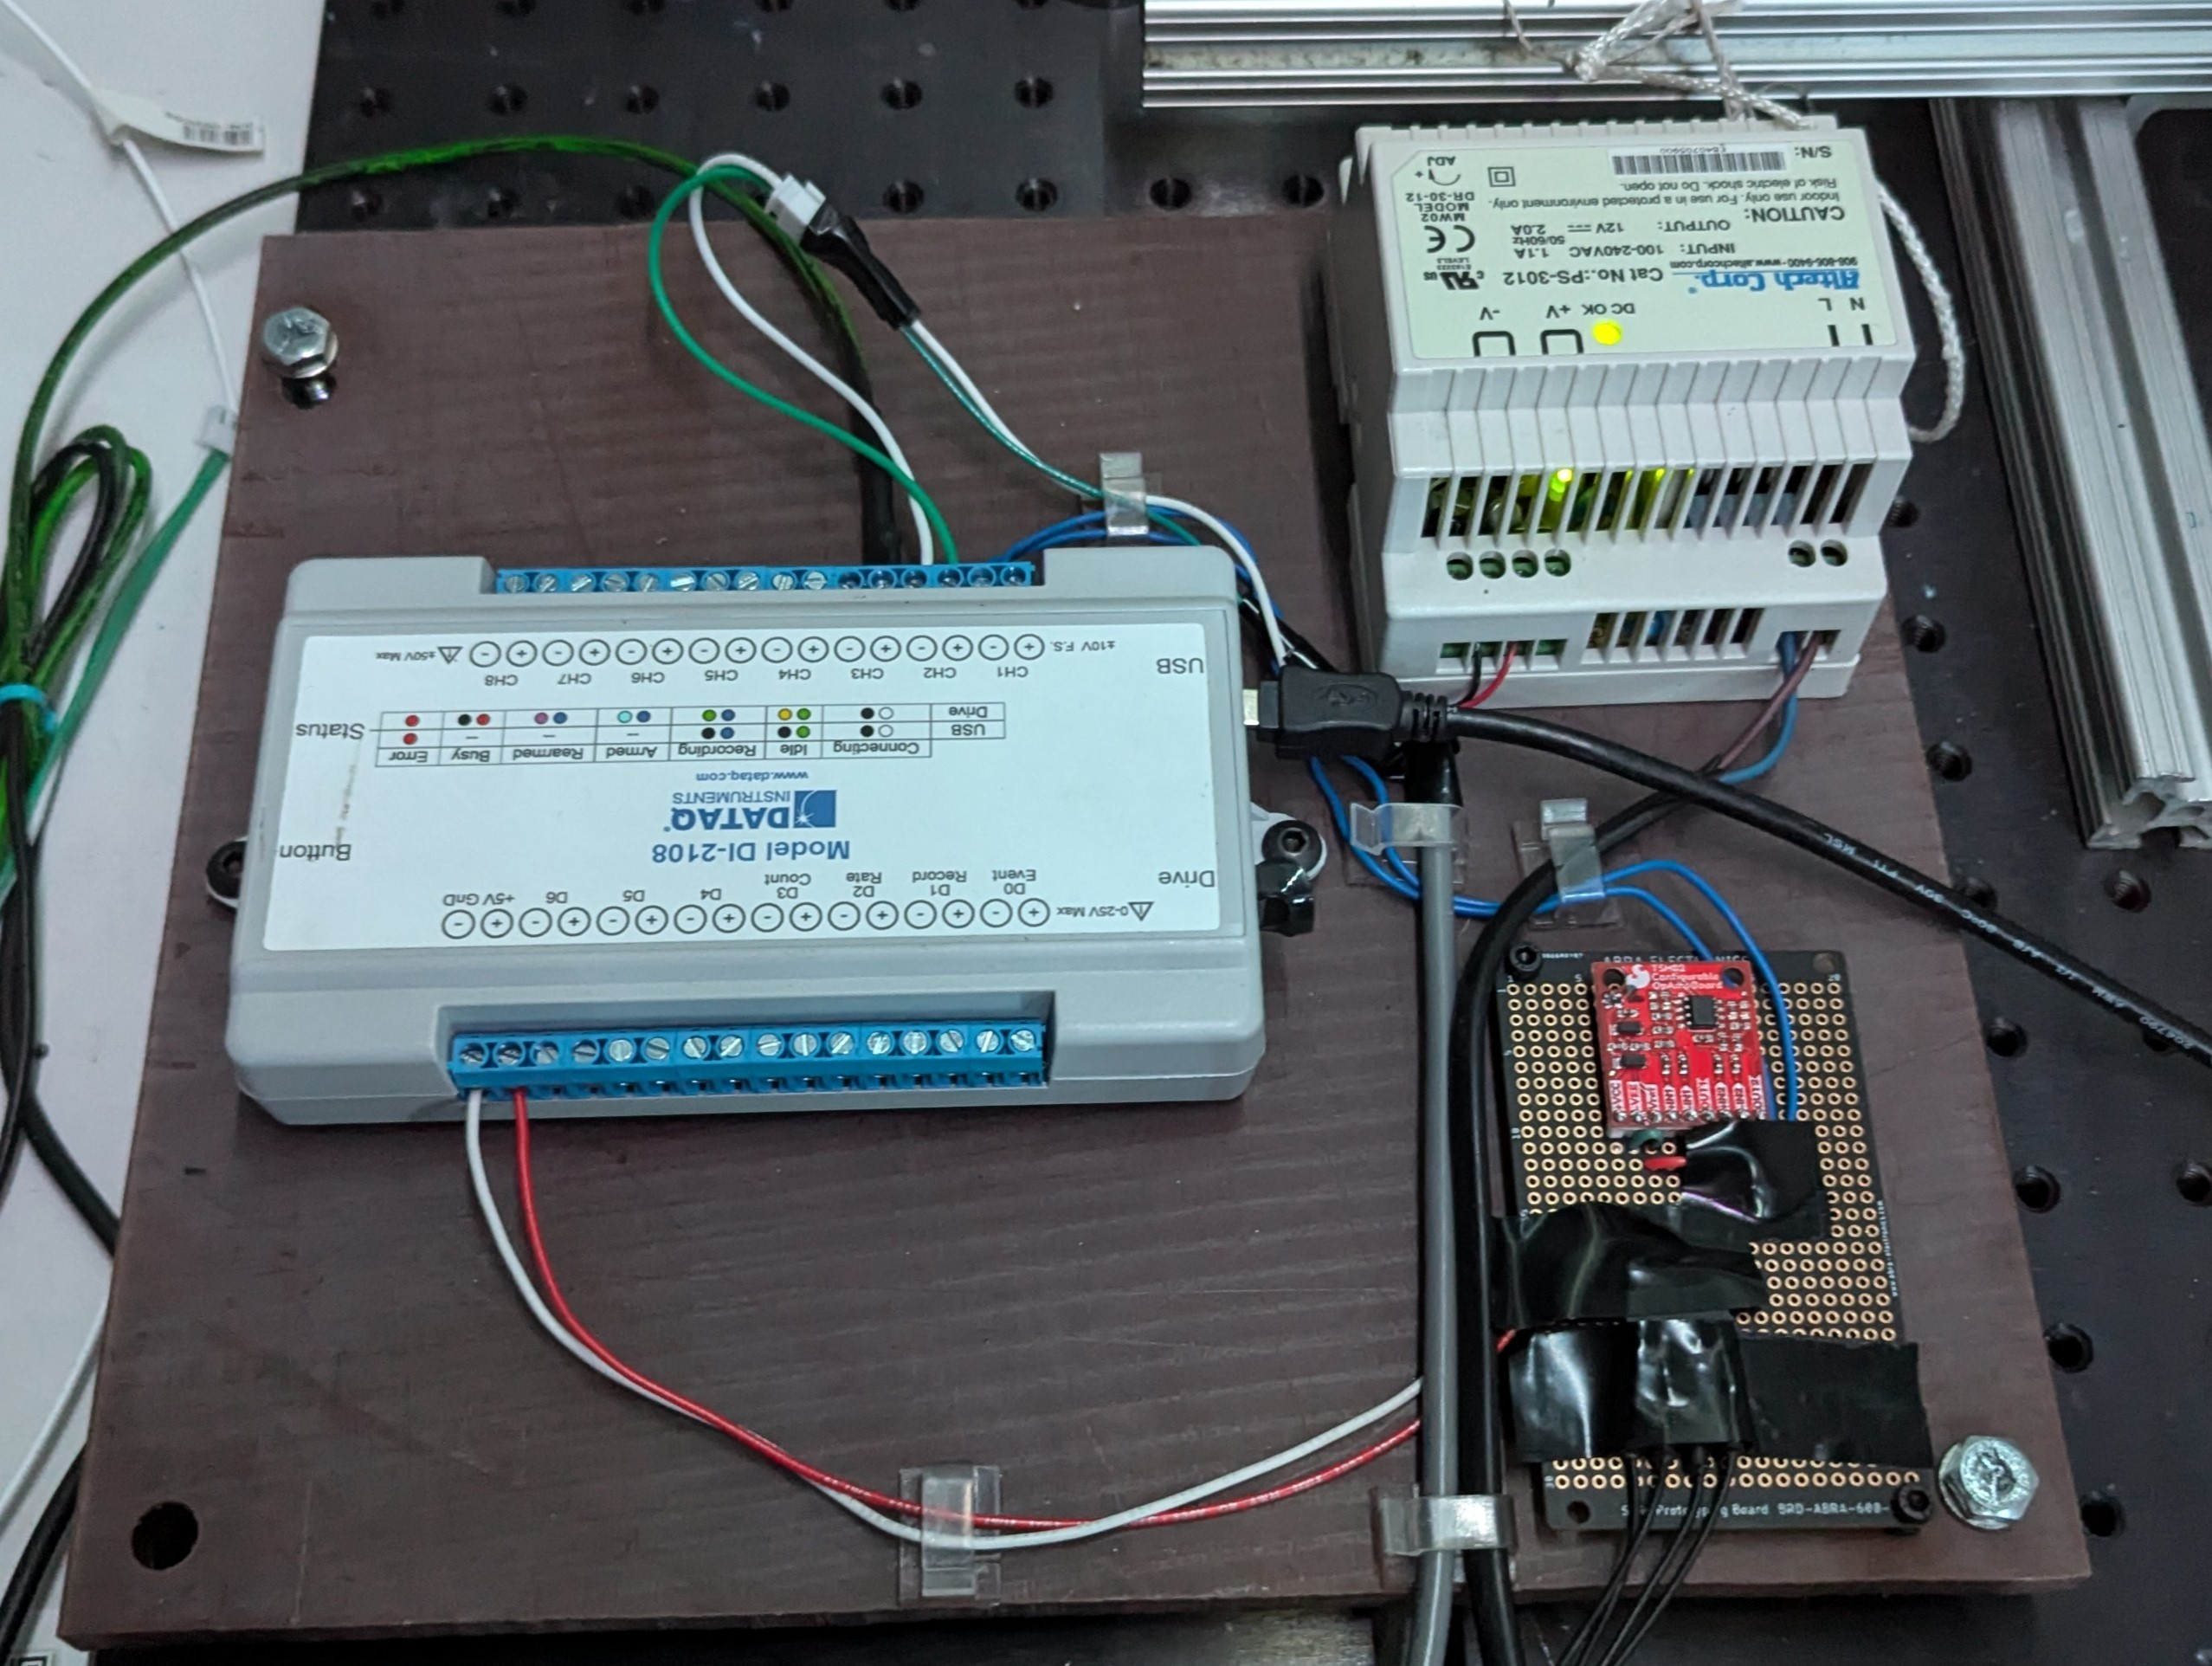
\includegraphics[width=0.50\textwidth]{assets/3 design/DAQ electronics.jpg}
                \caption{DAQ system}
                \label{fig:DAQ}
            \end{figure}

            [Photos of pressure sensor and PCB assembly]

        \subsection{High speed camera}

            A Photron SA5 high speed camera was used on certain LSP shots to validate 
            
            Due to the fact that no side window was present on V2, the Photron SA 5 high speed camera looking into the core of the thruster was used to validate.

            [Photo of Photron looking into thruster]
    \chapter{Experiments}

    The following chapter will explain the methodology and the results of the various experiments undertaken to develop, validate, and characterize the V2 thruster. Argon gas was used as the main propellant due to its low cost, safety, and ease of ionization.

    \section{Static LSP validation}

        \subsection{V1 LSP spark initiation}

            For spark initiation to work reliably, the laser focus and the spark must both be aligned in space and in time. To resolve the spark spatially, the Photron SA5 camera was placed in front of the V1 test section instead of the laser, looking axially into the test section. This would be the point of view of the laser collimator during a Laser-Supported Plasma (LSP) shot. \autoref{fig:spark composite} shows a composite photo of the added opacities of five spark discharges (without laser). Each frame of the video has an opacity of $1/N$, with $N$ being the total number of frames to add. This gave an average position of the spark, which is slightly to the left of the electrodes' centerline.

            \begin{figure}[!ht]
                \centering
                \begin{subfigure}[t]{0.25\textwidth}
                    \centering
                    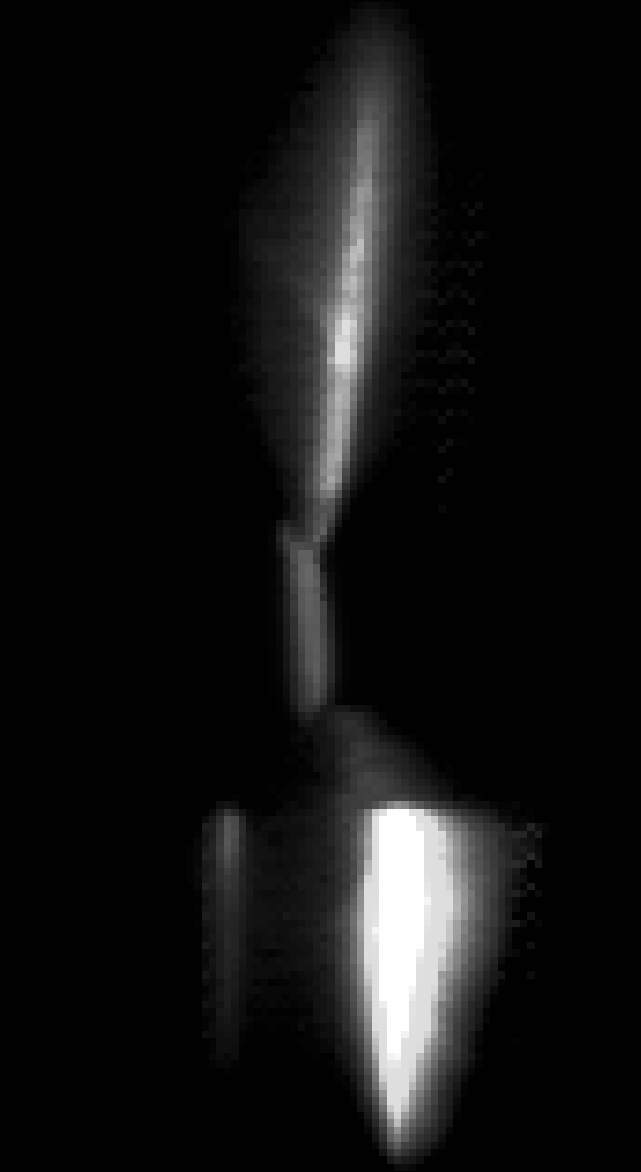
\includegraphics[width=\textwidth]{assets/4 experiments/Composite photo spark.png}
                    \caption{Composite photo showing spark between two electrodes. The spark gap is approximately \qty{0.8}{mm}.}
                    \label{fig:spark composite}
                \end{subfigure}
                \hfill
                \begin{subfigure}[t]{0.45\textwidth}
                    \centering
                    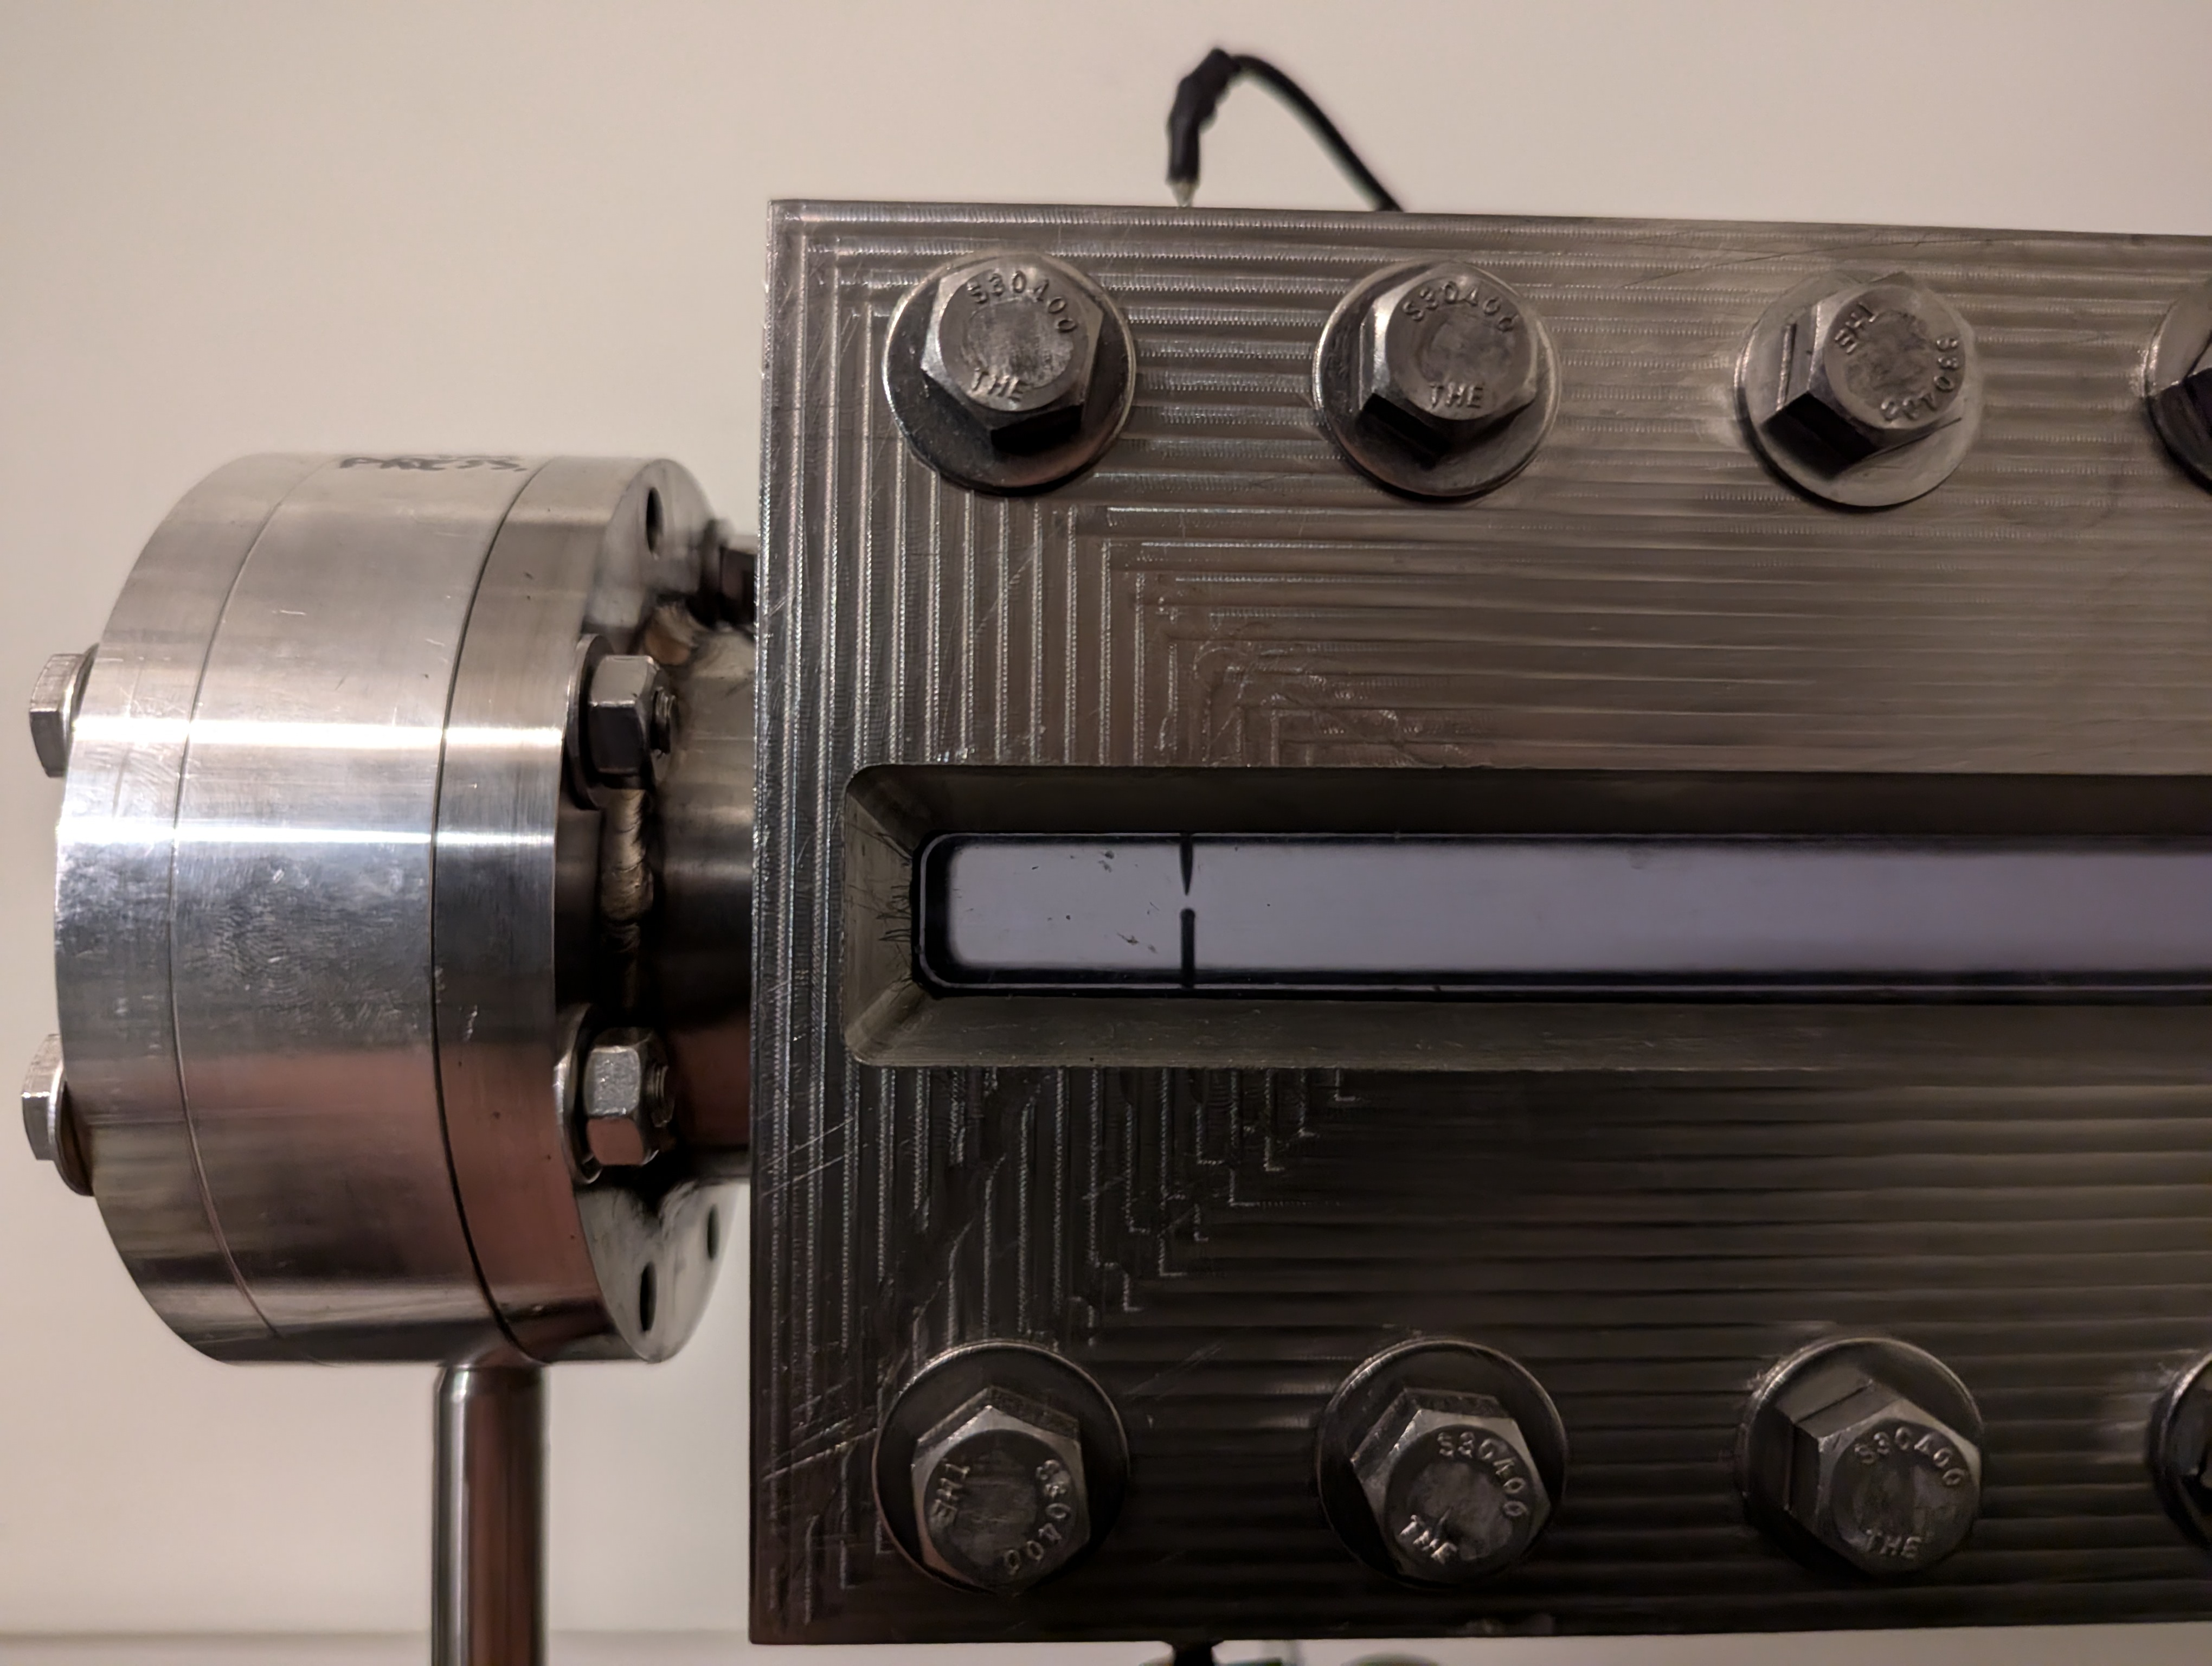
\includegraphics[width=\textwidth]{assets/4 experiments/V1 opposing electrodes.jpg}
                    \caption{Front of V1 test section showing electrode position. This view is rotated 90\degree from \autoref{fig:spark composite}}
                    \label{fig: standard view of electrodes}
                \end{subfigure}
                \caption{V1 spark alignment}
            \end{figure}
            
            Using the thickness of the electrode (\qty{1.55}{mm}) as a reference, the spark gap's length is \qty{0.8}{mm} and the average spark is \qty{0.2}{mm} wide. Timing data was also recorded for the spark by the high-speed camera. To align the laser focus to the spark in time, the laser was reinstalled, and the camera was placed back to its normal position looking into the side of the test section (as in \autoref{fig: standard view of electrodes}). The beam was then focused on one of the electrodes at low power. This caused the electrode to glow white-hot when the laser was on. The timings presented in \autoref{fig: Signal timing diagram} were determined by this investigation.

            \begin{figure}[!ht]
                \centering
                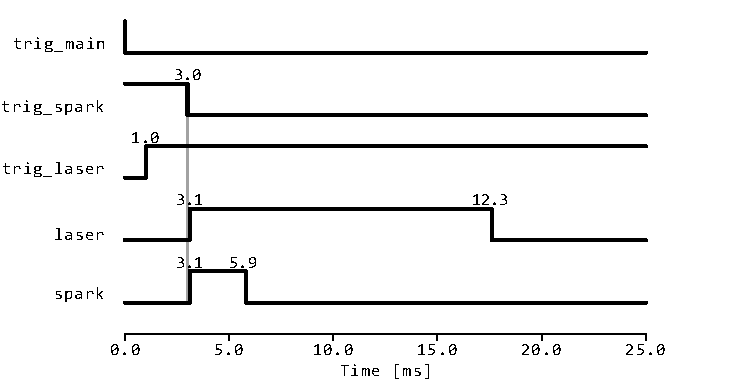
\includegraphics[width=0.75\textwidth]{assets/4 experiments/timings.pdf}
                \caption{Signal timing diagram. The \textit{trig} prefix denotes triggering signals. The component is active when the line is high. Timings in \unit{ms} are also indicated on the figure.}
                \label{fig: Signal timing diagram}
            \end{figure}

            With the position of the laser aligned to the spark and the timings synchronized, QCW LSP spark initiation in V1 was achieved with a \qty{200}{mm} focal length lens at 100\% power (\qty{3079}{W}) and a pressure of \qty{20}{bar}, as seen in \autoref{fig:V1_spark_initiation_frames}.
            
            \begin{figure}[h]
    \centering
    \begin{subfigure}[t]{0.3\textwidth}
        \centering
        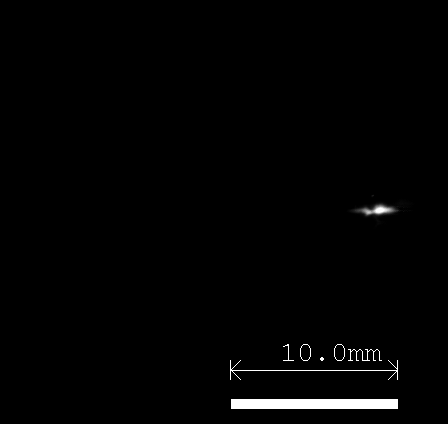
\includegraphics[width=\textwidth]{assets/4 experiments/V1 Spark Ignition Frames/LSP142_SPRK15_Fr32.bmp}
        \caption{\qty{3.2}{ms}}
        %\label{fig:V1_ignition_frames_16}
    \end{subfigure}
    \hfill
    \begin{subfigure}[t]{0.3\textwidth}
        \centering
        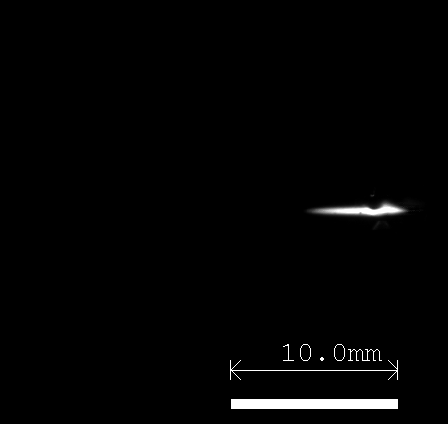
\includegraphics[width=\textwidth]{assets/4 experiments/V1 Spark Ignition Frames/LSP142_SPRK15_Fr33.bmp}
        \caption{\qty{3.3}{ms}}
        %\label{fig:ignition_frames_17}
    \end{subfigure}
    \hfill
    \begin{subfigure}[t]{0.3\textwidth}
        \centering
        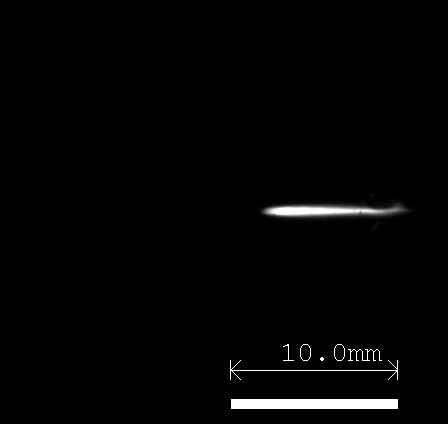
\includegraphics[width=\textwidth]{assets/4 experiments/V1 Spark Ignition Frames/LSP142_SPRK15_Fr35.bmp}
        \caption{\qty{3.5}{ms}}
        %\label{fig:ignition_frames_18}
    \end{subfigure}
    \begin{subfigure}[t]{0.3\textwidth}
        \centering
        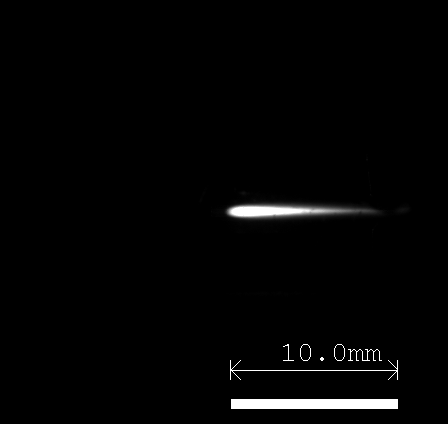
\includegraphics[width=\textwidth]{assets/4 experiments/V1 Spark Ignition Frames/LSP142_SPRK15_Fr38.bmp}
        \caption{\qty{3.8}{ms}}
        %\label{fig:ignition_frames_19}
    \end{subfigure}
    \hfill
    \begin{subfigure}[t]{0.3\textwidth}
        \centering
        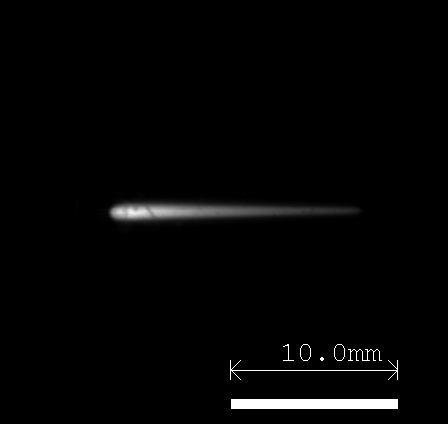
\includegraphics[width=\textwidth]{assets/4 experiments/V1 Spark Ignition Frames/LSP142_SPRK15_Fr69.bmp}
        \caption{\qty{6.9}{ms}}
        %\label{fig:ignition_frames_20}
    \end{subfigure}
    \hfill
    \begin{subfigure}[t]{0.3\textwidth}
        \centering
        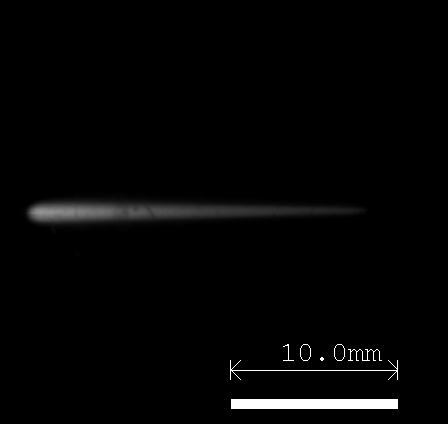
\includegraphics[width=\textwidth]{assets/4 experiments/V1 Spark Ignition Frames/LSP142_SPRK15_Fr130.bmp}
        \caption{\qty{13.0}{ms}}
        %\label{fig:ignition_frames_21}
    \end{subfigure}
    \caption{LSP spark initiation: \qty{3080}{W}, \qty{20}{bar}. \shotsettings{LSP142\_SPRK15}{0.1?? CHANGE}{22}{2048}}
    \label{fig:V1_spark_initiation_frames}
\end{figure}
            
            The LSP is initiated at \qty{3.2}{ms}, as soon as the spark is discharged. The front of the LSP moves towards the left (upstream, towards the laser), until the end of the QCW laser pulse at \qty{13}{ms}. Once the laser ends its emission, the LSP dies down within two frames (\qty{0.2}{ms}).
            % I could include here the dynamic pressure rise of the LSP.

        \subsection{\ce{NO2} seeding}

            % If you want to present the NO2 work, you'll need to: Explain attenuation/absorption coefficient as it appears in Beer-Lambert law and how this defines the length scale over which absorption occurs. Explain how absorption coefficient is derived from the cross-section of the molecule, which will involve using the HITRAN database, etc. It is not acceptable to just say "we added NO2" and reference it off to some paper.}
            
            As the plasma emits in the ultraviolet (UV) range, it is necessary to seed with a gas that absorbs UV but not the infrared (IR) laser. \textcite{khanGasDetectionUsing2019} shows that \ce{NO2} and \ce{SO2} are two candidates. \ce{NO2} was first used as it was easy to produce in-house in significant quantities. The V1 system was set up with a vacuum pump connected to an outside air exhaust to safely vent the \ce{NO2} gas. The pump was also used to bring the pressure in the test section down to a rough vacuum before introducing the gasses.

            %[Add absorption spectrum of NO2 from Gas Detection Using Portable Deep-UV Absorption Spectrophotometry: A Review or other place]

            Three control QCW LSP shots were done in pure argon and their dynamic pressure trace from the PCB transducer was recorded. Next, 0.55 bar of \ce{NO2}, or 200 mL at STP, was introduced into the chamber. V1 was then pressurized with argon to 20 bar. With the spark active, three LSPs were generated in the seeded atmosphere. The dynamic pressure rise of the seeded argon was approximately double the one seen in pure argon. The next two LSP shots were conducted with 0.24 bar (\qty{85}{ml} at STP) of \ce{NO2} and filled to 20.2 bar with argon. Again, higher pressure increases were observed, but slightly less than the \qty{0.55}{bar} shots. The chamber was finally half evacuated to 10.17 bar and then filled back to \qty{20.15}{bar} with argon. This would have brought the partial pressure of \ce{NO2} to \qty{0.12}{bar}. Two LSPs were initiated, with a higher pressure increase than pure argon, but less than the higher concentration \ce{NO2} shots. \autoref{fig:NO2_shots_analysis} presents the averages of these recorded pressure traces.

            \begin{figure}[!ht]
                \centering
                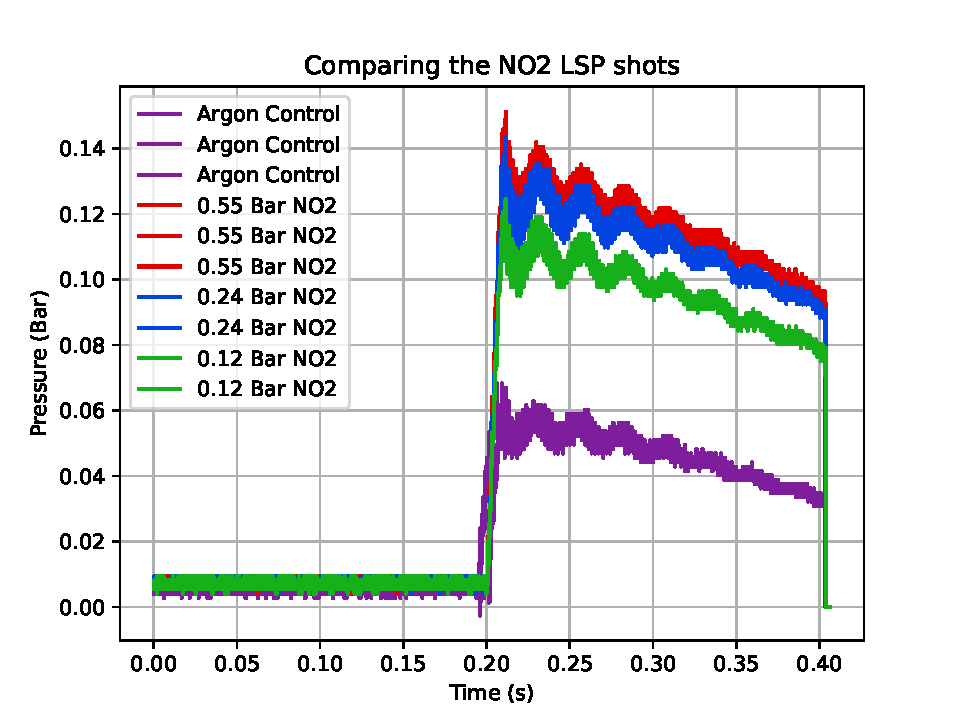
\includegraphics[width=0.75\textwidth]{assets/4 experiments/NO2_shots_analysis.pdf}
                \caption{Average dynamic pressure rise of QCW LSP shots in a mixture of \ce{NO2} and argon compared to that of pure argon QCW LSP. Initial pressure was \qty{20.15}{bar}. Values given in the legend are the partial pressure of \ce{NO2} seeding in the gas.}
                \label{fig:NO2_shots_analysis}
            \end{figure}

        \subsection{V2 LSP spark initiation and QCW LSP}

            For V2, the timings of the spark and laser pulse were kept the same as \autoref{fig: Signal timing diagram}. To align the laser focus spatially, the power meter was used as a screen to project the visible (red) alignment laser. By moving the V2 test section back and forth on the thrust stand rail, the field of view (FOV) of the shadows projected on the power meter can be modified, as seen in \autoref{fig:FOV}. The laser focus can then be moved with the translation stages, so the brightest spot matches the center of the electrodes' shadow.
            
            \begin{figure}[!ht]
                \centering
                \begin{subfigure}[t]{0.45\textwidth}
                    \centering
                    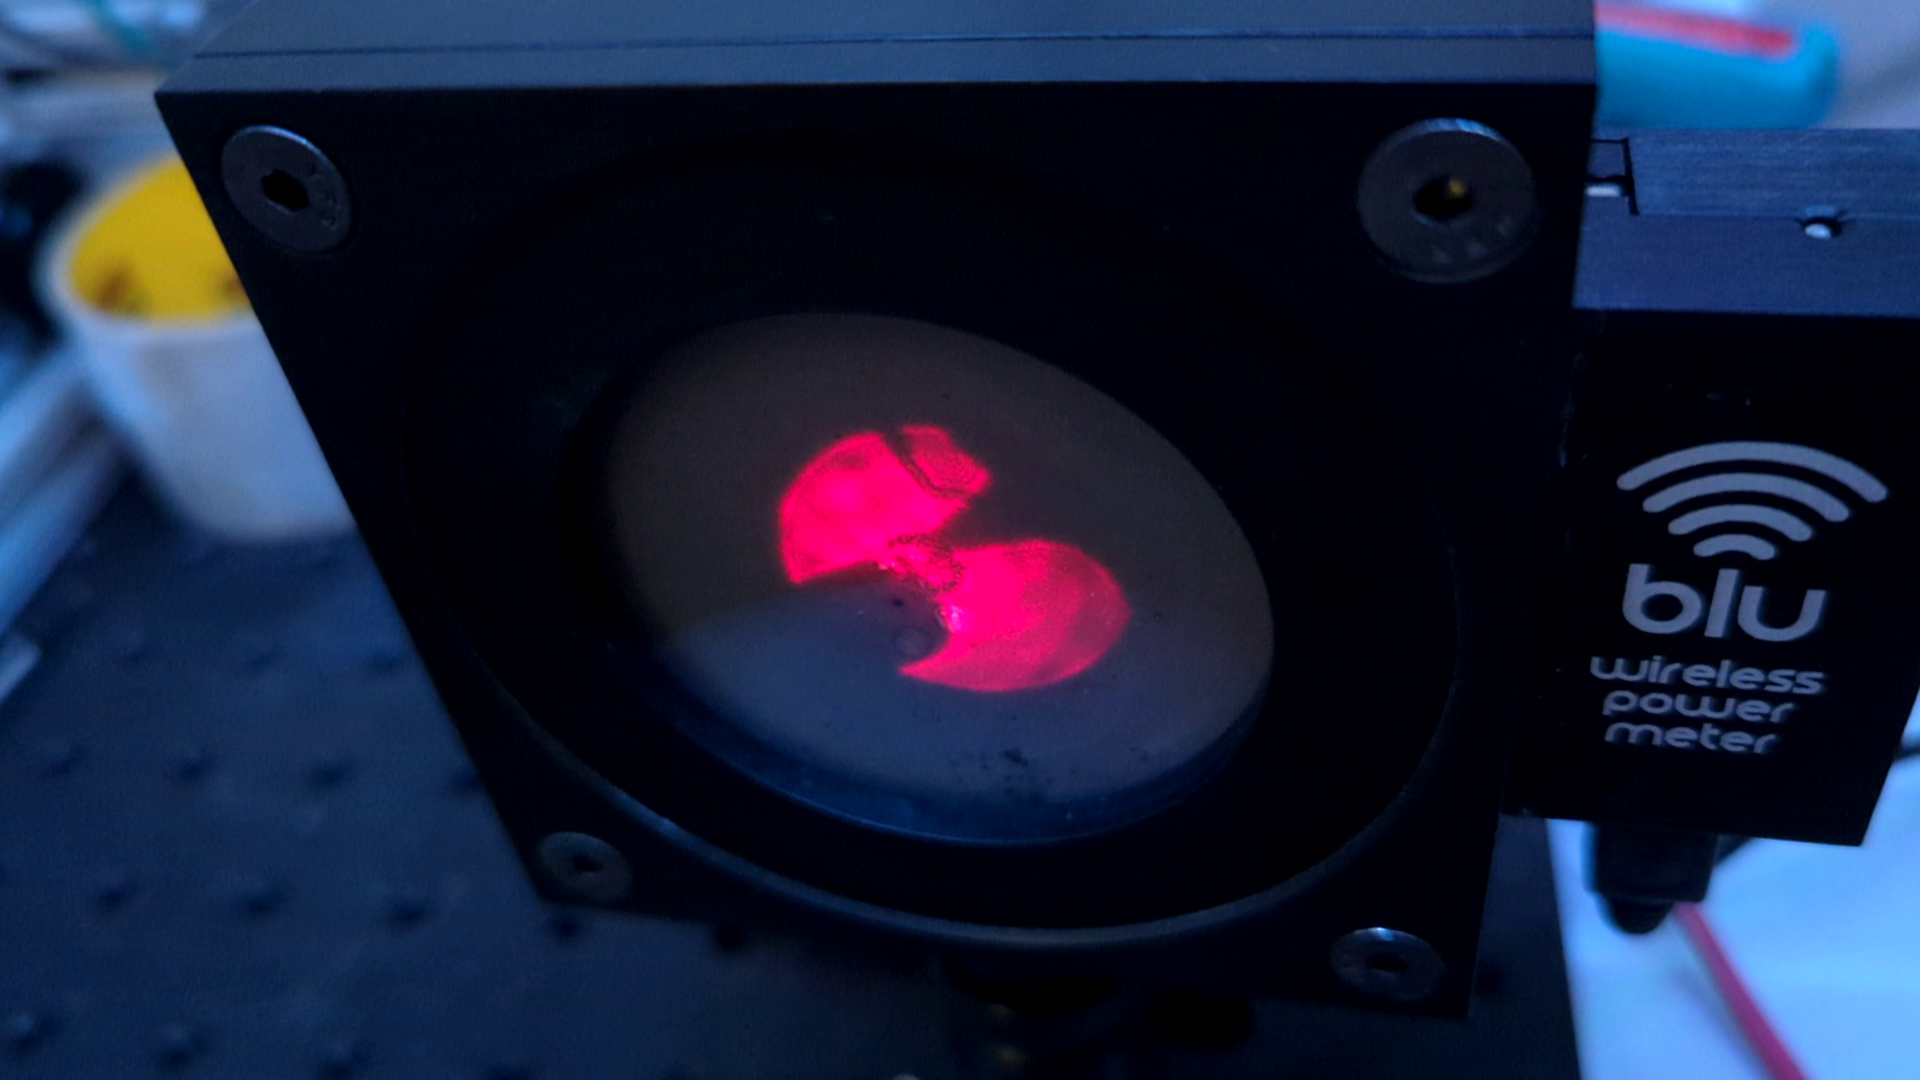
\includegraphics[width=\textwidth]{assets/4 experiments/V2 alignment 1.png}
                    \caption{V2 alignment, zoomed out}
                \end{subfigure}
                \hfill
                \begin{subfigure}[t]{0.45\textwidth}
                    \centering
                    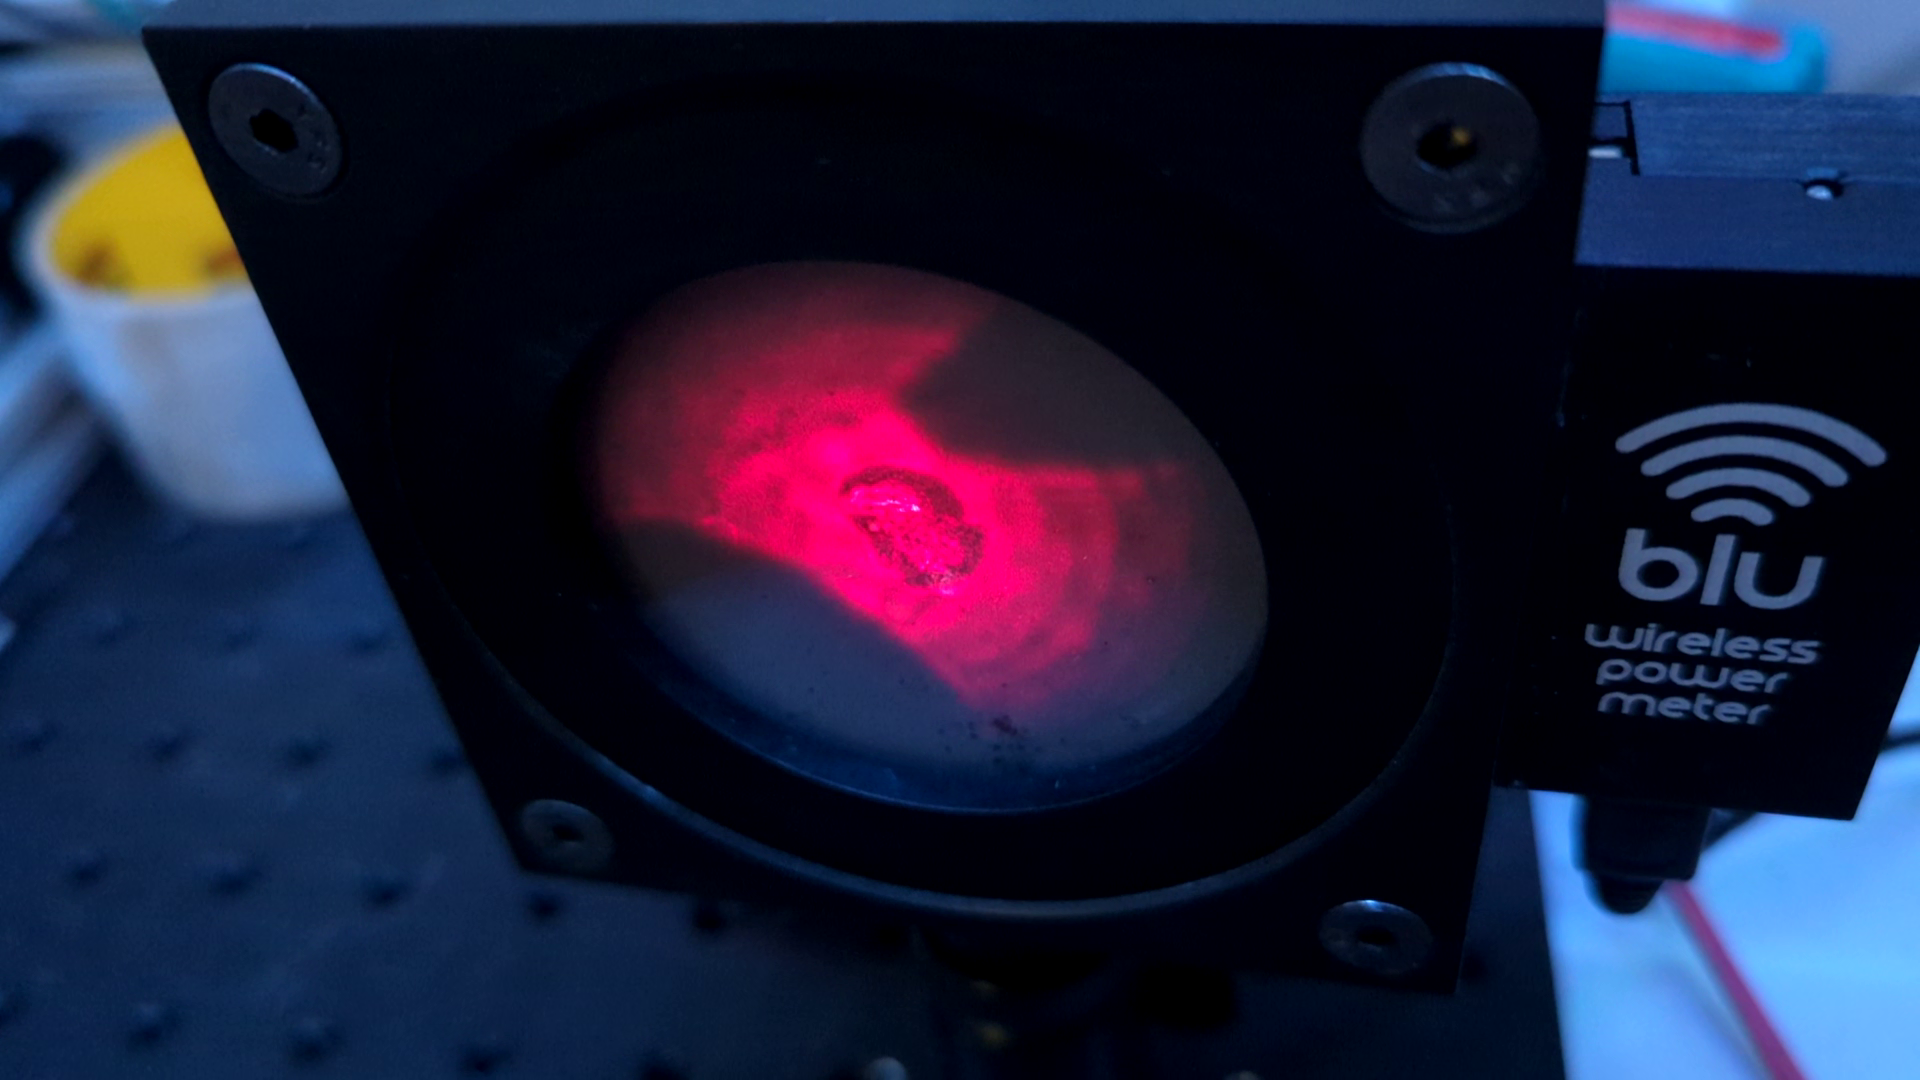
\includegraphics[width=\textwidth]{assets/4 experiments/V2 alignment 2.png}
                    \caption{V2 alignment, zoomed in}
                \end{subfigure}
                \caption{2 FOVs of alignment laser light on power meter. The aberration at the center of the red light is due to laser damage to the window.}
                \label{fig:FOV}
            \end{figure}

            Once the laser focus was aligned, QCW LSP initiation was confirmed in V2 by the Photron SA5 looking into the front of the thruster at an angle, and the PCB transducer recording the pressure rise. \autoref{fig: big flash}, taken by the webcam, shows the brightness of a full power QCW LSP. Note the bright plasma emission to the left of the image on the laser safety curtain.

            \begin{figure}[!ht]
                \centering
                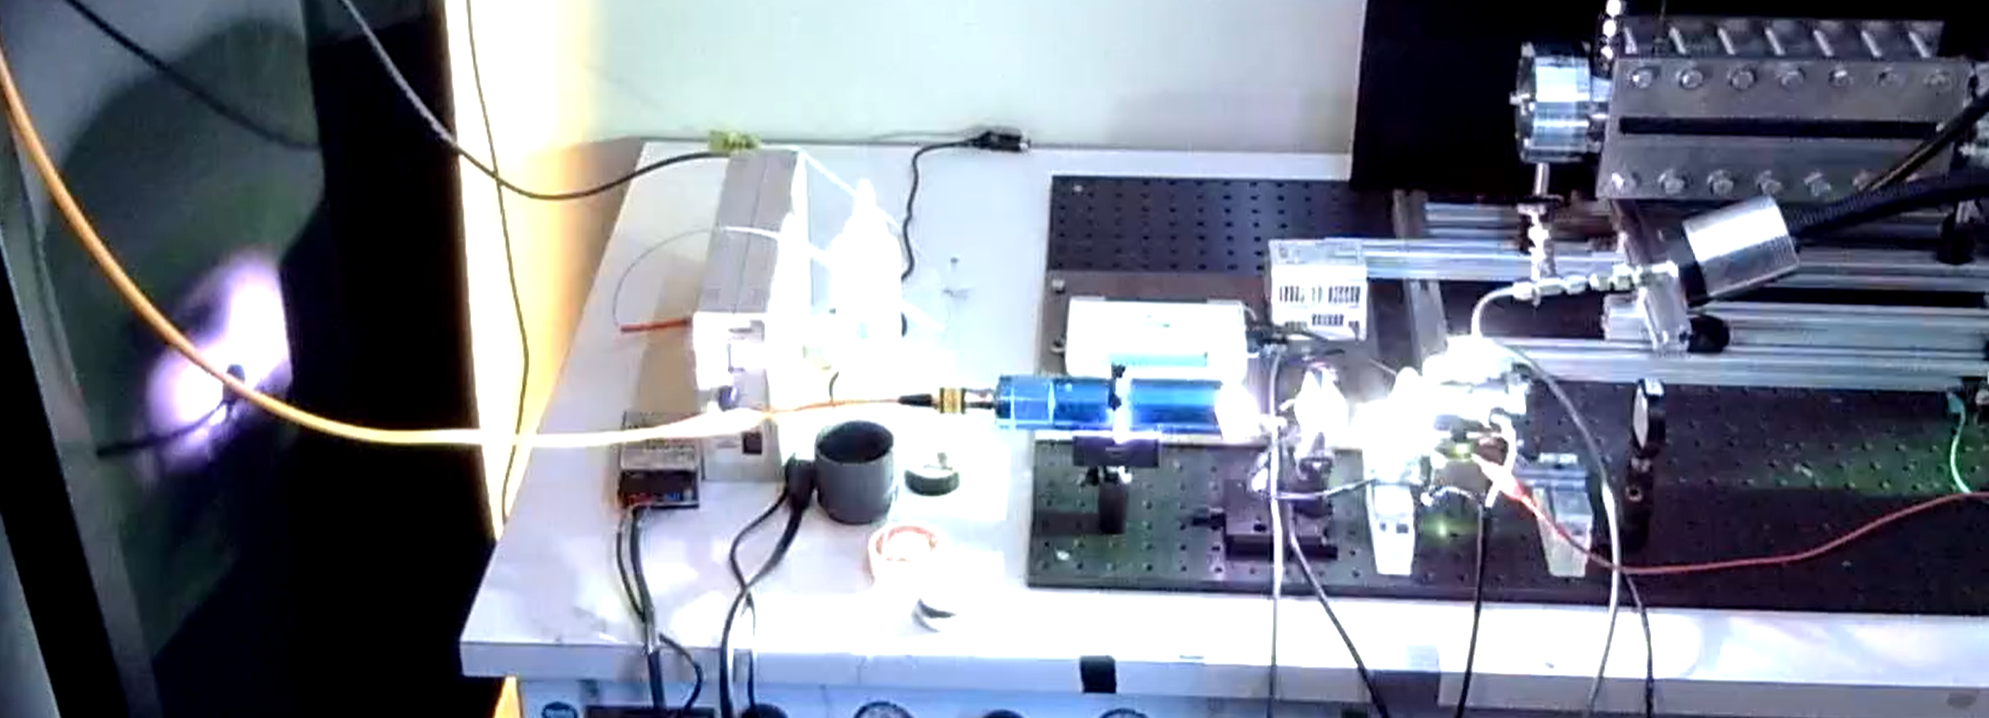
\includegraphics[width=\textwidth]{assets/4 experiments/holy jesus look at this.png}
                \caption{100\% power (\qty{3079}{W}) QCW LSP shot}
                \label{fig: big flash}
            \end{figure}

        \subsection{Optical experiments: going from QCW to CW LSP}

            Due to the low continuous laser power in this experiment compared to others in the literature, increasing the laser flux with a small focus is critical. The real amount of power in the pulsed shots was measured to get a conversion between the laser power setting (in \%) to power (W), which does not scale directly at lower powers. 10 shots each at \qtylist{10; 12}{\%} were measured with the power meter, with statistics compiled by the power meter software (\autoref{tab:laser shot statistics}). The average power was calculated by dividing the average pulse energy (J) by the pulse duration (\qty{50}{ms}).

            \begin{table}[!ht]
                \caption{Statistics from the power meter after 10 times \qty{50}{ms} laser shots at \qty{10}{\%} and \qty{12}{\%} power}
                \label{tab:laser shot statistics}
                \begin{tabular}{lll}
                \textbf{Value {[}Unit{]}} & \textbf{10 $\times$ \qty{50}{ms} shots at 10\% power} & \textbf{10 $\times$ \qty{50}{ms} shots at 12\% power} \\ \hline
                Average energy value {[}J{]}  & 9.985 & 12.89 \\
                Maximum energy value {[}J{]}  & 10.2  & 13.3  \\
                Minimum energy value {[}J{]}  & 9.63  & 12.0  \\
                RMS Stability {[}\%{]} & 1.690 & 2.811 \\
                PTP Stability {[}\%{]} & 5.599 & 10.31 \\
                Std deviation {[}J{]}  & 0.169 & 0.362 \\
                Average power {[}W{]}  & 200 & 258  \\ \hline
                \end{tabular}
            \end{table}
            
            Extrapolating from these results, \qty{300}{W} is achieved at \qty{13.5}{\%}.

            %first V1 test
            Pulsed shots at lower power levels with a \qty{200}{mm} focal length lens (Thorlabs LA1979-C) revealed a difficulty to initiate QCW LSP below \qty{30}{\%} power, around \qty{1}{kW}. This presented a problem, as the maximum continuous wave (CW) power of the laser is significantly lower at \qty{342}{W} (see \autoref{chp:app_YLR}). A test campaign was initiated to determine if LSP initiation in the V1 thruster was possible under this maximum CW power level. \autoref{eqn: spot diameter} \cite{LaserSpotSize} can be used to estimate the beam diameter at the focus:
            
            \begin{equation}\label{eqn: spot diameter}
                \text{Spot diameter (mm)} = \frac{4 \times \text{Focal length (mm)} \times \text{Wavelength (mm)}\times M^2}{\pi \times \text{Beam diameter at lens (mm)}}
            \end{equation}

            The beam propagation factor $M^2$ is a scale to measure beam quality. A diffraction-limited Gaussian beam has the minimum $M^2$ of 1 (\textcite{hechtUnderstandingLasersEntry2019}). The YLR-300/3000 laser has a Beam Parameter Product (BPP) of \qty{2}{mm.mrad}, as found in \autoref{chp:app_YLR}. As $M^2 = \frac{\pi}{\lambda} \text{BPP}$ \cite{paschottaBeamParameterProduct}, this corresponds to an $M^2$ of 5.87. From \autoref{eqn: spot diameter}, lowering the focal length of the lens lowers the spot diameter, increasing laser flux. The \textit{Thorlabs} \textcite{LensTutorial} also mentions that a dual-lens system can lower the beam diameter at the focus.

            A single plano-convex lens with a \qty{125}{mm} focal length (Thorlabs LA1384-C) was then used, as it was the lowest focal length lens that could focus at V1's initiation plug position. A \qty{100}{mm} focal length lens was available, but the position of the focus was before the electrodes, even when pressing the lens against V1's front window. \autoref{fig: 125mm focus threshold} shows a record of LSP initiation attempts at various power settings and lens axial positions with the \qty{125}{mm} focal length lens. An argon pressure of \qty{20}{bar} was used for these shots.
            \begin{figure}[!ht]
                \centering
                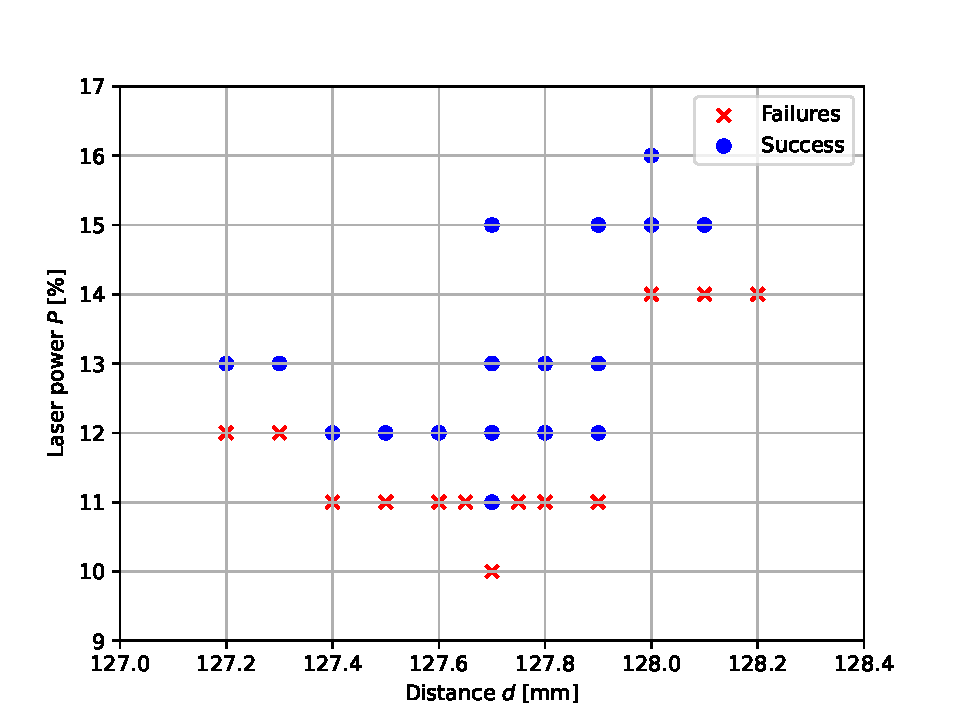
\includegraphics[width=0.75\textwidth]{assets/4 experiments/125mm_focus_threshold.pdf}
                \caption{LSP threshold graph for V1 with \qty{125}{mm} focal length lens}
                \label{fig: 125mm focus threshold}
            \end{figure}
            At power levels lower than 15\%, initiation was unreliable and could take up to 20 attempts to get one initiation. For example, initiation at \qty{11}{\%} was successful once, but it was not possible to repeat this. An even smaller diameter focus was necessary to increase initiation reliability by increasing laser flux at the focus, and a dual-lens system was designed.

            For a dual-lens system, the spot diameter must be calculated numerically. Ray tracing software, such as WinLens3D Basic, calculate the geometry of paraxial \footnote{Rays having small angles and distances to the optical axis} rays and show the path of these rays at the focus. WinLens3D was chosen to simulate the spot size of both the single- and dual-lens systems, as it is free and powerful enough for this application. The modelled lenses are seen in \autoref{fig:modeled lenses}.
            \begin{figure}[!ht]
                \centering
                \begin{subfigure}[t]{0.45\textwidth}
                    \centering
                    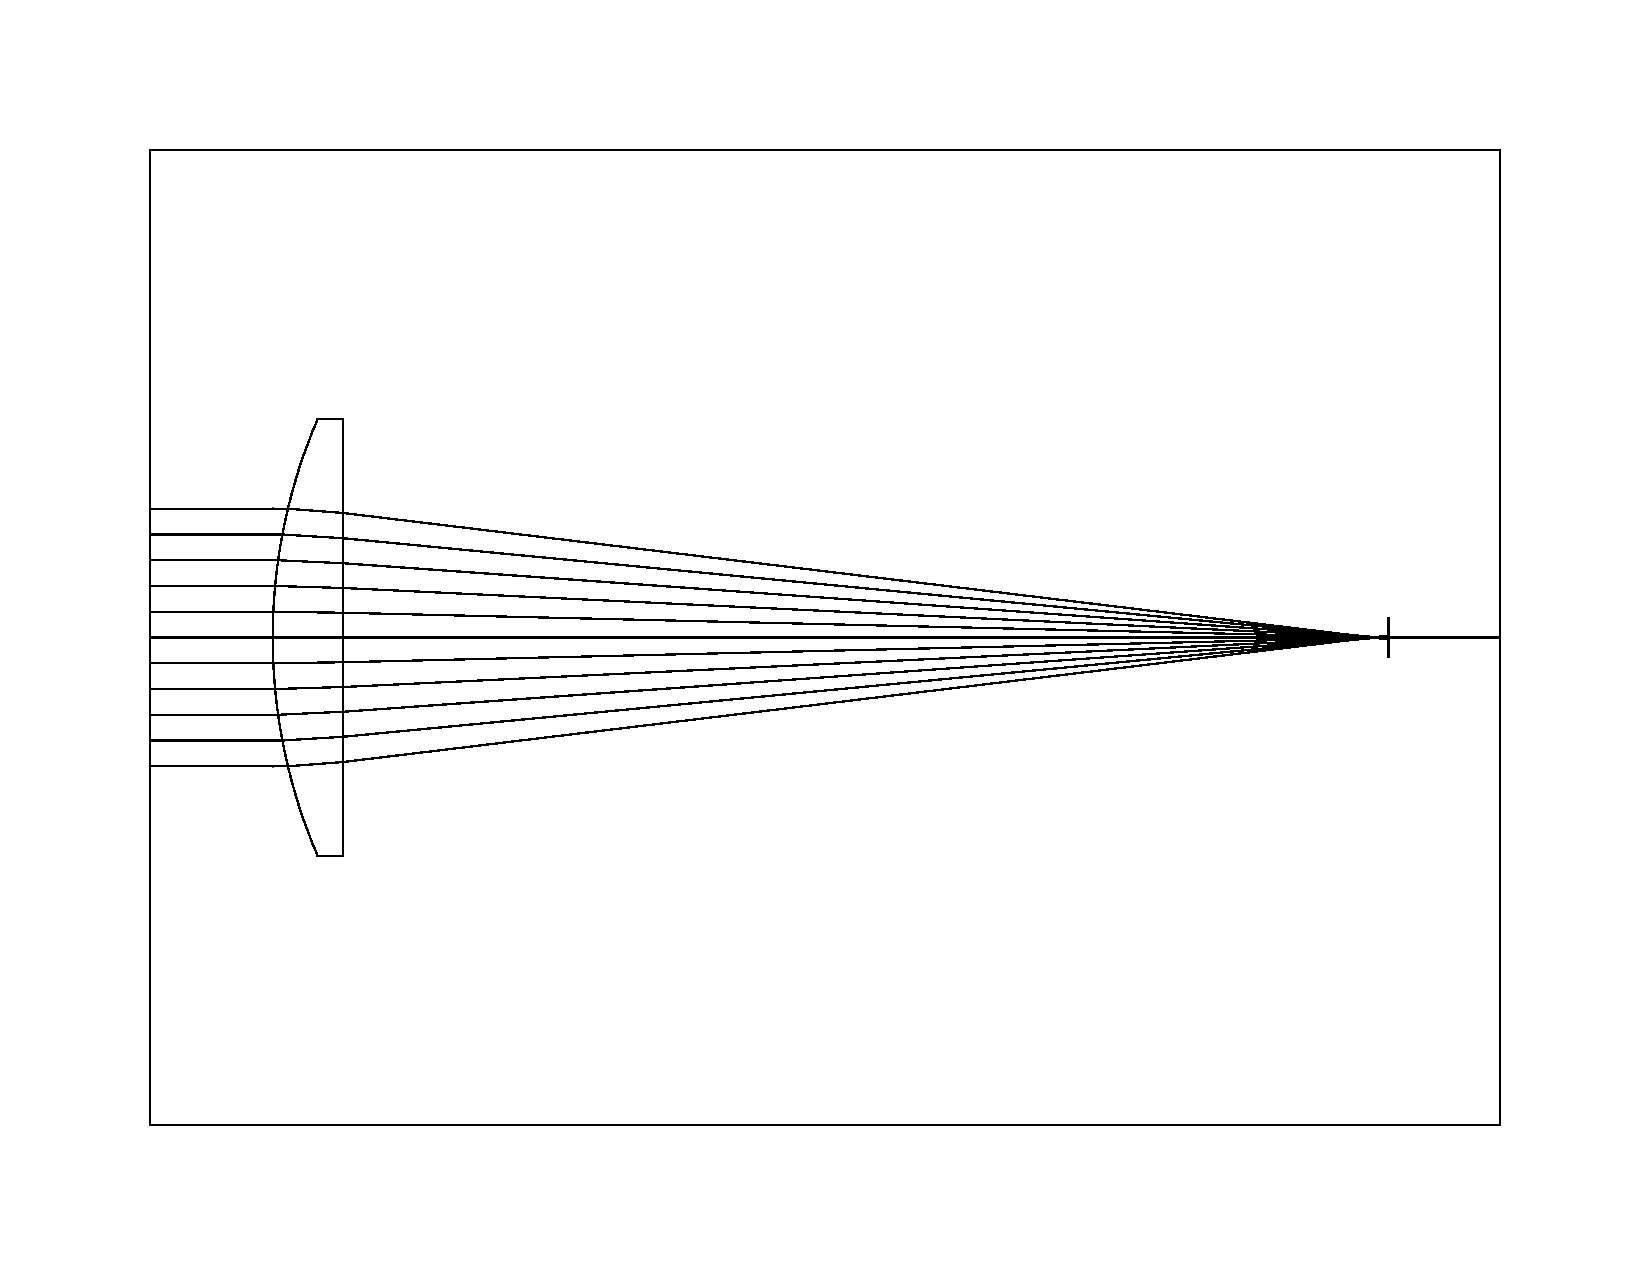
\includegraphics[width=\textwidth]{assets/4 experiments/125lens.pdf}
                    \caption{\qty{125}{mm} focal length lens}
                \end{subfigure}
                \hfill
                \begin{subfigure}[t]{0.45\textwidth}
                    \centering
                    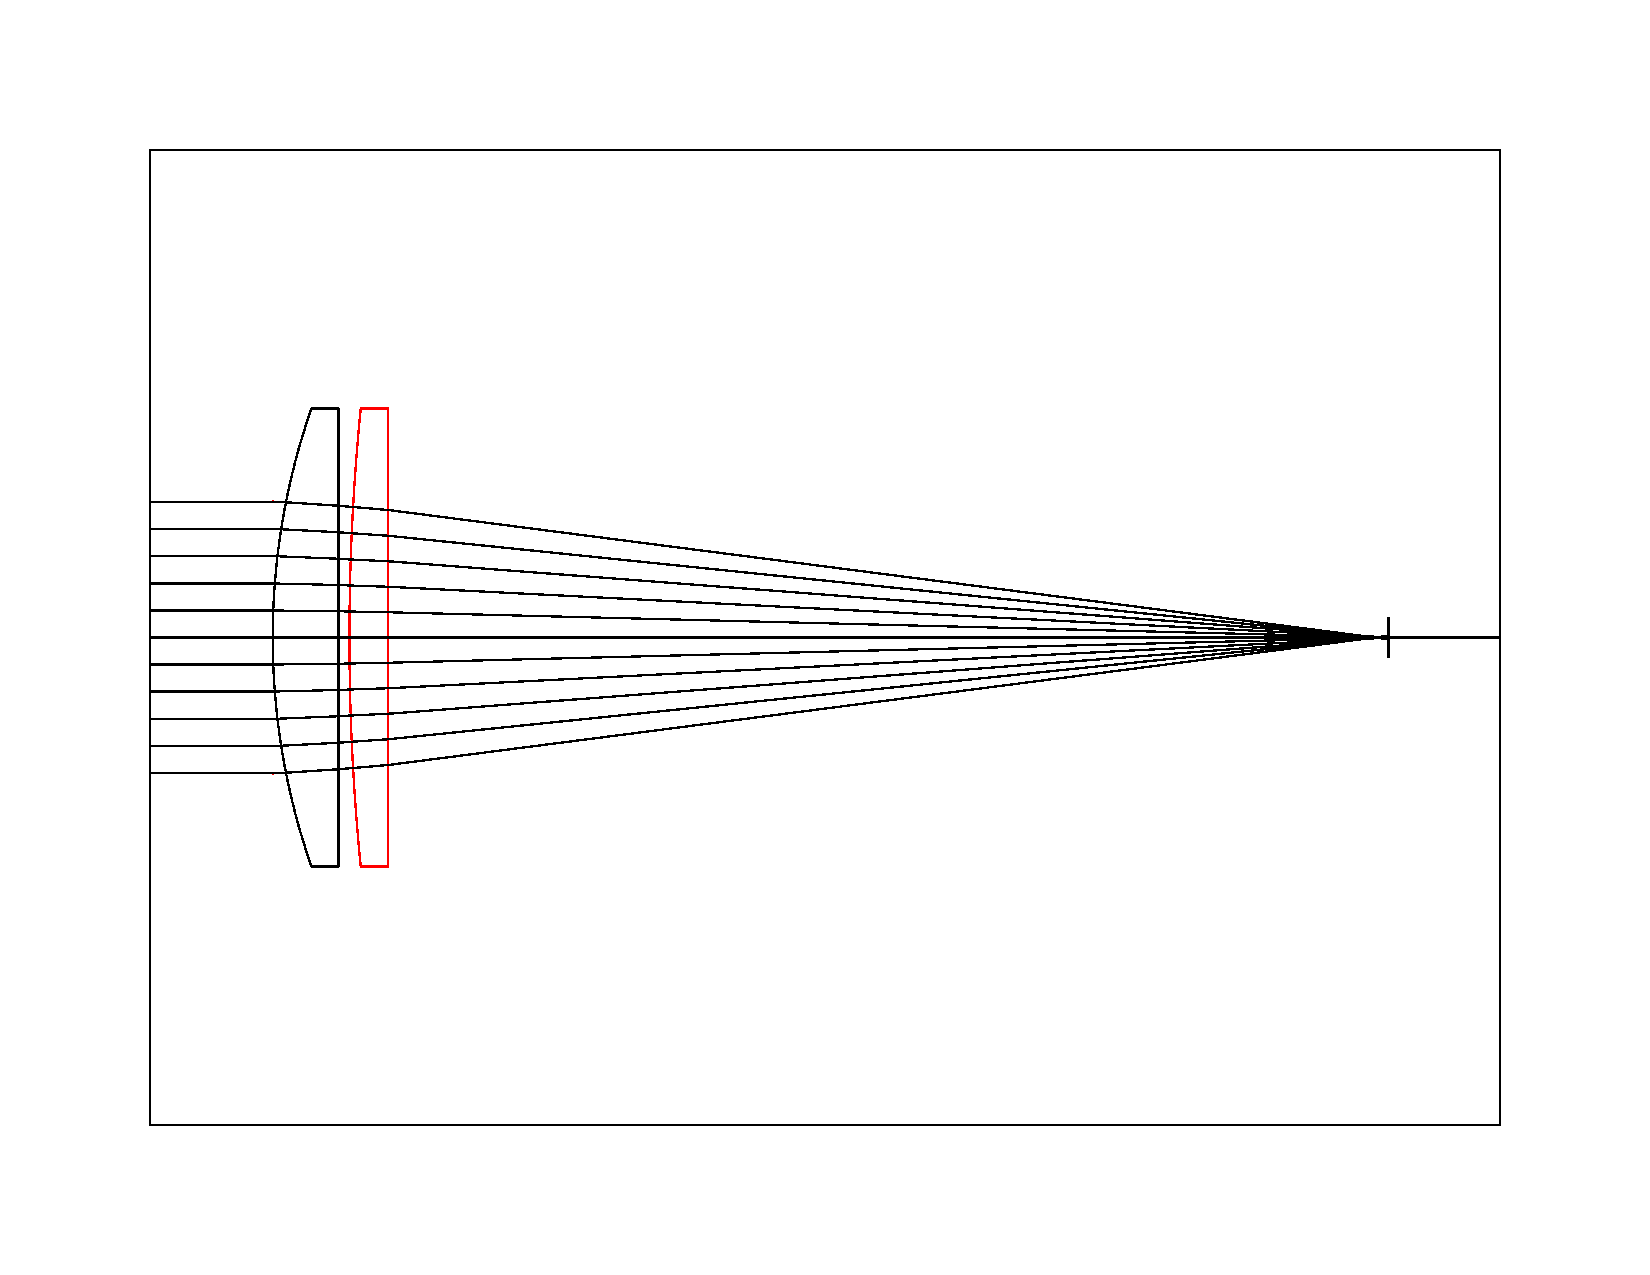
\includegraphics[width=\textwidth]{assets/4 experiments/500 and 150 lenses.pdf}
                    \caption{Dual-lens \qtylist{500;150}{mm} system}
                \end{subfigure}
                \caption{Model of the lenses showing paraxial rays and focus}
                \label{fig:modeled lenses}
            \end{figure}

            With a dual-lens system, the longest focal length lens should be placed first, contrary to what is shown. This would lead to a tighter focus, as the diameter of the beam entering the second lens is maximized. In this case, the \qty{500}{mm} focal length lens was placed after the \qty{150}{mm} lens as it was impossible to mount before with the available mounting hardware. WinLens3D showed that the difference in spot size was minimal. A practical consideration for the experiments is that the LSP will be formed upstream of the laser focus when there is no gas flow because the plasma's radiation pre-heats the gas. Therefore, the focus needs to be slightly after the initiation system.

            \autoref{fig:spot diagrams} presents the spot diagrams that were then produced with WinLens3D. Note the difference in scales and spacing used throughout.
            \begin{figure}[!ht]
                \centering
                \begin{subfigure}[t]{\textwidth}
                    \centering
                    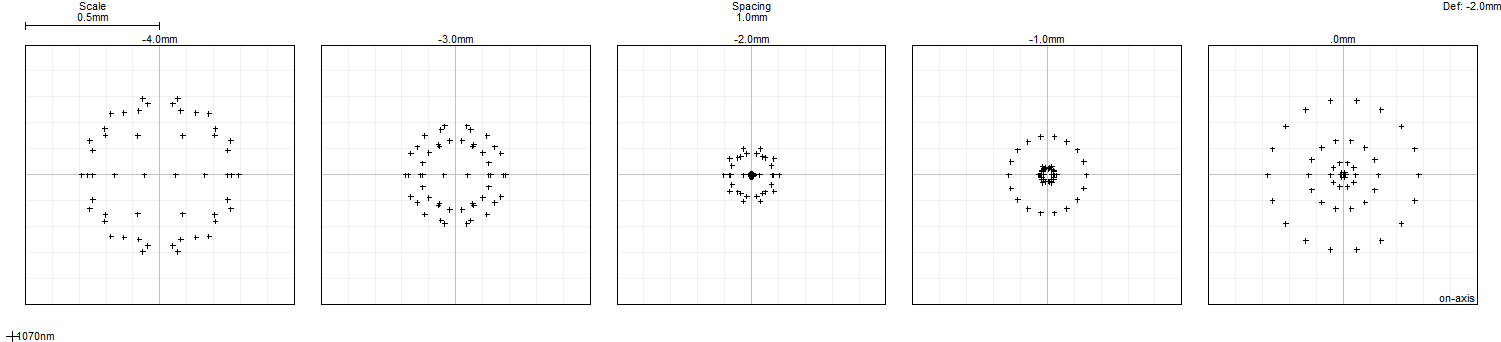
\includegraphics[width=\textwidth]{assets/3 design/100 lens spot diagram.png}
                    \caption{\qty{100}{mm} focal length lens}
                \end{subfigure}
                \begin{subfigure}[t]{\textwidth}
                    \centering
                    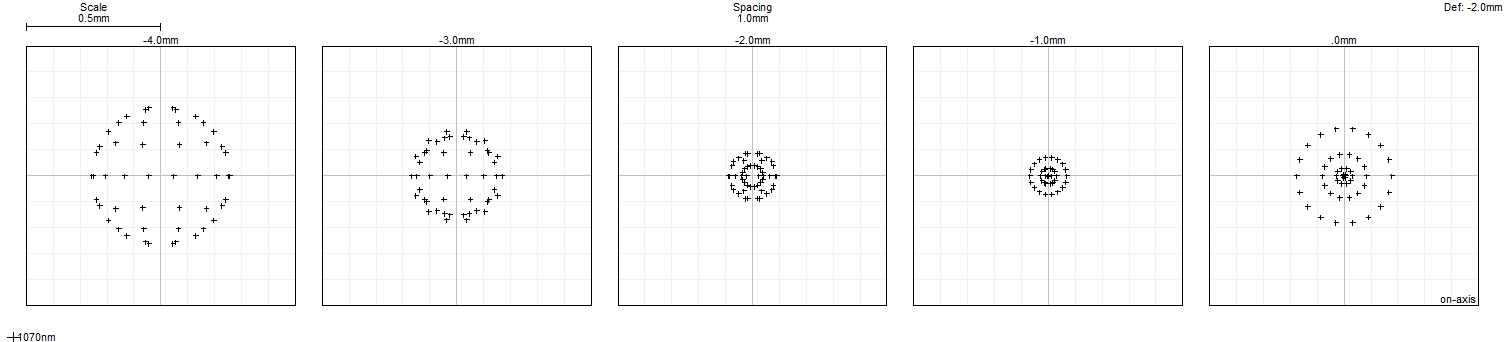
\includegraphics[width=\textwidth]{assets/3 design/125 lens spot diagram.png}
                    \caption{\qty{125}{mm} focal length lens}
                \end{subfigure}
                \begin{subfigure}[t]{\textwidth}
                    \centering
                    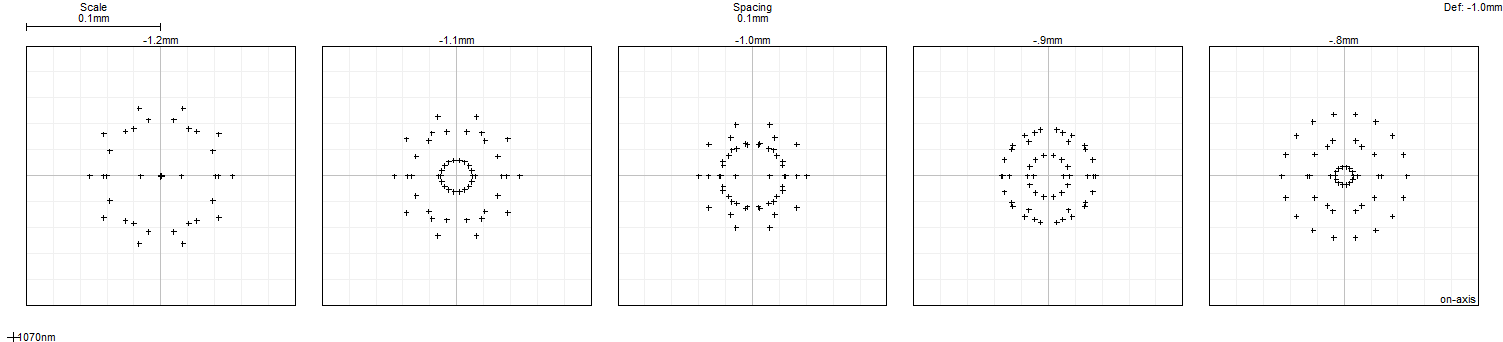
\includegraphics[width=\textwidth]{assets/3 design/500 and 150 lenses spot size.png}
                    \caption{Dual-lens \qtylist{500;150}{mm} system}
                \end{subfigure}
                \caption{Spot diagrams of the three lens systems studied}
                \label{fig:spot diagrams}
            \end{figure}
            From these three spot diagrams, the average laser flux at \qtylist{342}{W} was calculated (see \autoref{tab:laser flux}). It is assumed that the laser energy is evenly distributed in a circle as wide as the farthest ray from the center, which gives a lower bound for the laser flux.
            \begin{table}[!ht]
                \centering
                \caption{Simulated focal length and spot diameter of various lens assemblies in WinLens3D. The average laser flux is calculated for \qty{342}{W} of incident power}
                \label{tab:laser flux}
                \begin{tabularx}{\textwidth}{@{}lX<{\raggedright}X<{\raggedright}X<{\raggedright}X<{\raggedright}@{}}
                \toprule
                Lens & Nominal focal length (\unit{mm}) & Focal length at \qty{1070}{nm} (\unit{mm})& Beam diameter at focus (\unit{mm}) & Average laser flux at \qty{342}{W} (\unit{MW/cm^2}) \\ \midrule
                Single & 125           &  122  &    0.20   &  1.09 \\
                Single & 100           &  93   &    0.15   &  1.94 \\
                Dual & 500, 150      &  110  &    0.08   &  6.80 \\ %calculations for this in C:\Users\gdub5\Documents\WinLens Files
                \bottomrule
                \end{tabularx}
            \end{table}
            The LSP experiments were continued with this dual-lens system (\qty{500}{mm} and \qty{150}{mm} focal lengths), as it offers a 6.25 times increase of the laser flux compared to the single \qtylist{125}{mm} focal length lens. To increase the laser flux even more, an aspheric lens of comparable focal length could be used, though it costs 10 times as much as a single plano-convex lens. \autoref{fig:V1 dual-lens threshold graph} presents a record of LSP initiation attempts at various power settings and lens axial positions with this dual-lens system in V1.
            \begin{figure}[!ht]
                \centering
                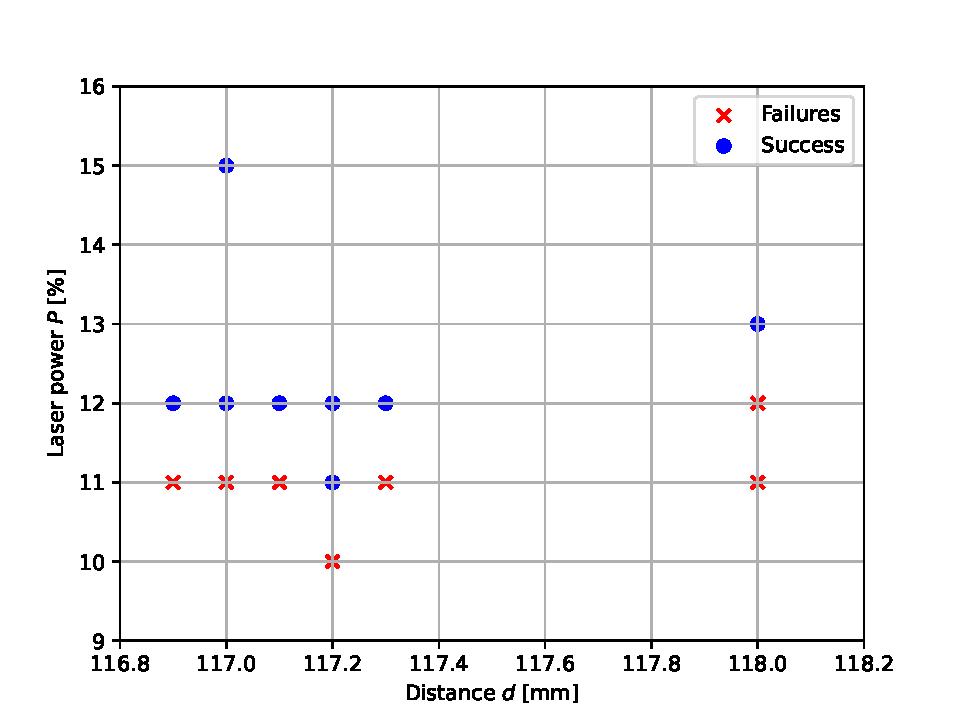
\includegraphics[width=0.75\textwidth]{assets/4 experiments/duallens_focus_threshold.pdf}
                \caption{LSP threshold graph for V1 with dual-lens system}
                \label{fig:V1 dual-lens threshold graph}
            \end{figure}
            The completion of these tests validated the dual-lens design, showing that LSPs in the CW power regime of the laser could be generated. The first LSPs in V2 were therefore done using the dual-lens system. A similar graph to \autoref{fig:V1 dual-lens threshold graph} was then created with V2 to find the lens position where the minimum laser power could reliably initiate QCW LSP. \autoref{fig:V2 threshold graph} presents these initiation attempts.
            \begin{figure}[!ht]
                \centering
                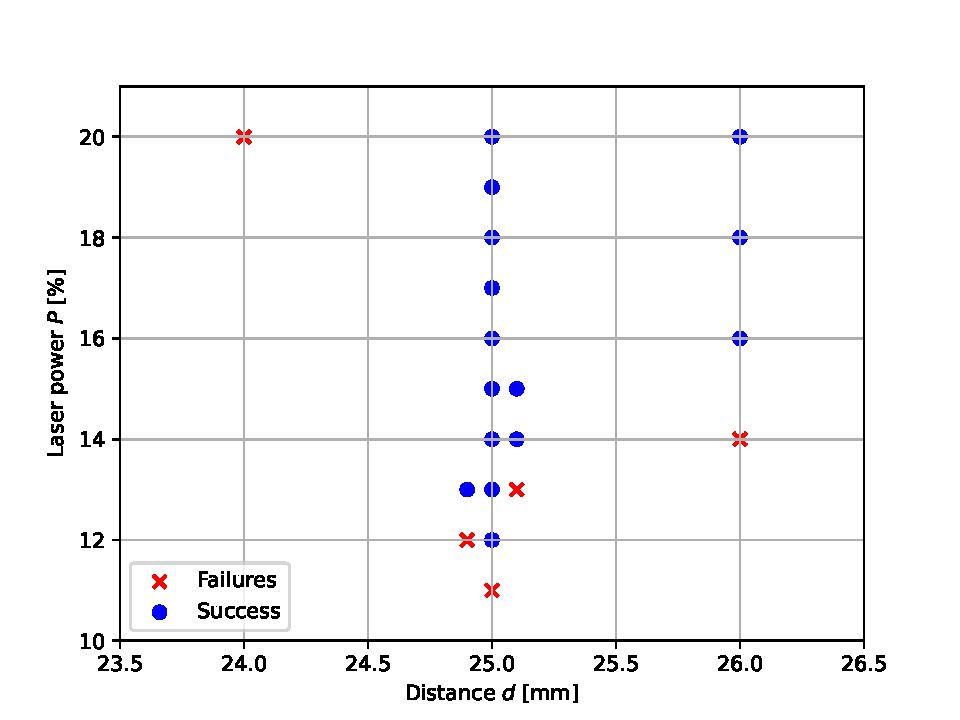
\includegraphics[width=0.75\textwidth]{assets/4 experiments/V2_focus_threshold.pdf}
                \caption{LSP threshold graph for V2 with dual-lens system}
                \label{fig:V2 threshold graph}
            \end{figure}

        \subsection{V2 CW LSP}

            A \qty{100}{\%} power CW shot was then attempted with static argon at \qty{20}{bar}. 

            \begin{figure}[h]
    \centering
    \begin{subfigure}[t]{0.3\textwidth}
        \centering
        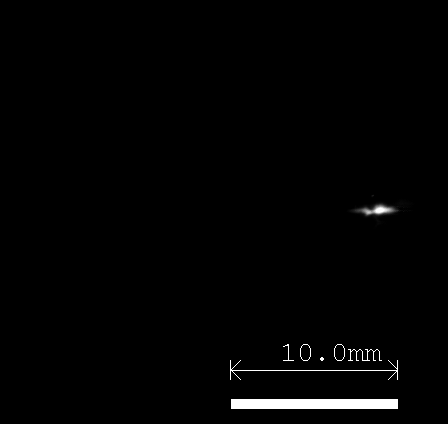
\includegraphics[width=\textwidth]{assets/4 experiments/V1 Spark Ignition Frames/LSP142_SPRK15_Fr32.bmp}
        \caption{\qty{3.2}{ms}}
        %\label{fig:V1_ignition_frames_16}
    \end{subfigure}
    \hfill
    \begin{subfigure}[t]{0.3\textwidth}
        \centering
        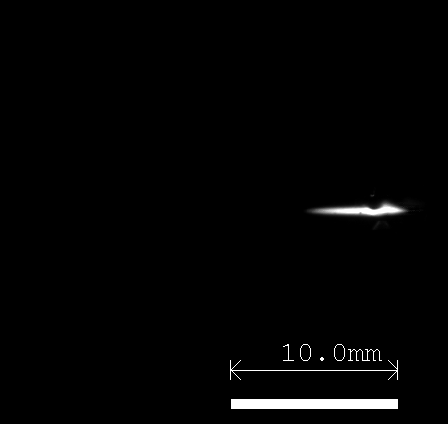
\includegraphics[width=\textwidth]{assets/4 experiments/V1 Spark Ignition Frames/LSP142_SPRK15_Fr33.bmp}
        \caption{\qty{3.3}{ms}}
        %\label{fig:ignition_frames_17}
    \end{subfigure}
    \hfill
    \begin{subfigure}[t]{0.3\textwidth}
        \centering
        \includegraphics[width=\textwidth]{assets/4 experiments/V1 Spark Ignition Frames/LSP142_SPRK15_Fr35.bmp}
        \caption{\qty{3.5}{ms}}
        %\label{fig:ignition_frames_18}
    \end{subfigure}
    \begin{subfigure}[t]{0.3\textwidth}
        \centering
        \includegraphics[width=\textwidth]{assets/4 experiments/V1 Spark Ignition Frames/LSP142_SPRK15_Fr38.bmp}
        \caption{\qty{3.8}{ms}}
        %\label{fig:ignition_frames_19}
    \end{subfigure}
    \hfill
    \begin{subfigure}[t]{0.3\textwidth}
        \centering
        \includegraphics[width=\textwidth]{assets/4 experiments/V1 Spark Ignition Frames/LSP142_SPRK15_Fr69.bmp}
        \caption{\qty{6.9}{ms}}
        %\label{fig:ignition_frames_20}
    \end{subfigure}
    \hfill
    \begin{subfigure}[t]{0.3\textwidth}
        \centering
        \includegraphics[width=\textwidth]{assets/4 experiments/V1 Spark Ignition Frames/LSP142_SPRK15_Fr130.bmp}
        \caption{\qty{13.0}{ms}}
        %\label{fig:ignition_frames_21}
    \end{subfigure}
    \caption{LSP spark initiation: \qty{3080}{W}, \qty{20}{bar}. \shotsettings{LSP142\_SPRK15}{0.1?? CHANGE}{22}{2048}}
    \label{fig:V1_spark_initiation_frames}
\end{figure}

            The webcam footage (\autoref{fig:CW_V2_webcam_frames}) will be examined first. The laser is first turned on. A flash marks the spark initiation and lifetime of the LSP. This flash lasts only a few frames. Notice the higher brightness in \autoref{fig:CW_V2_webcam_frames_LSP}, reflecting off various surfaces like the white box (PCB signal conditioner) on the left of the collimator. The laser was kept running for about a second before it was turned off.

            \begin{figure}[h]
    \centering
    \begin{subfigure}[t]{0.3\textwidth}
        \centering
        \includegraphics[width=\textwidth]{assets/4 experiments/V1 Spark Ignition Frames/LSP142_SPRK15_Fr32.bmp}
        \caption{\qty{3.2}{ms}}
        %\label{fig:V1_ignition_frames_16}
    \end{subfigure}
    \hfill
    \begin{subfigure}[t]{0.3\textwidth}
        \centering
        \includegraphics[width=\textwidth]{assets/4 experiments/V1 Spark Ignition Frames/LSP142_SPRK15_Fr33.bmp}
        \caption{\qty{3.3}{ms}}
        %\label{fig:ignition_frames_17}
    \end{subfigure}
    \hfill
    \begin{subfigure}[t]{0.3\textwidth}
        \centering
        \includegraphics[width=\textwidth]{assets/4 experiments/V1 Spark Ignition Frames/LSP142_SPRK15_Fr35.bmp}
        \caption{\qty{3.5}{ms}}
        %\label{fig:ignition_frames_18}
    \end{subfigure}
    \begin{subfigure}[t]{0.3\textwidth}
        \centering
        \includegraphics[width=\textwidth]{assets/4 experiments/V1 Spark Ignition Frames/LSP142_SPRK15_Fr38.bmp}
        \caption{\qty{3.8}{ms}}
        %\label{fig:ignition_frames_19}
    \end{subfigure}
    \hfill
    \begin{subfigure}[t]{0.3\textwidth}
        \centering
        \includegraphics[width=\textwidth]{assets/4 experiments/V1 Spark Ignition Frames/LSP142_SPRK15_Fr69.bmp}
        \caption{\qty{6.9}{ms}}
        %\label{fig:ignition_frames_20}
    \end{subfigure}
    \hfill
    \begin{subfigure}[t]{0.3\textwidth}
        \centering
        \includegraphics[width=\textwidth]{assets/4 experiments/V1 Spark Ignition Frames/LSP142_SPRK15_Fr130.bmp}
        \caption{\qty{13.0}{ms}}
        %\label{fig:ignition_frames_21}
    \end{subfigure}
    \caption{LSP spark initiation: \qty{3080}{W}, \qty{20}{bar}. \shotsettings{LSP142\_SPRK15}{0.1?? CHANGE}{22}{2048}}
    \label{fig:V1_spark_initiation_frames}
\end{figure}

            Observation of the high-speed camera footage (\autoref{fig:CW_V2_Photron_frames}), recorded at 10,000 frames per second, showed the CW LSP starting at frame 32 (\qty{3.2}{ms}) and ending at frame 883 (\qty{88.3}{ms}), lasting \qty{85.1}{ms}. This represents a 1.7 times longer lifetime than the maximum QCW pulse length of \qty{50.0}{ms} at this power. The brightness of the plasma increases regularly after initiation, to reach its maximum intensity around \qty{50}{ms}. The maximum brightness is constant for \qty{10}{ms}. A flickering of the LSP is seen at \qty{70.0}{ms}, before it died down and was completely extinguished after \qty{88.3}{ms}. This was the first CW LSP generated in the lab.

            \begin{figure}[!ht]
                \centering
                \includegraphics[width=0.75\textwidth]{assets/4 experiments/CW pressure rise.pdf}
                \caption{Dynamic pressure rise from CW LSP measured with PCB transducer}
                \label{fig:CW pressure rise}
            \end{figure}

            \autoref{fig:CW pressure rise} shows the pressure rise recorded by the PCB transducer connected to the oscilloscope. Minimal damage to the window was noticed after this test.

        % \subsection{CW power measurement}

        %     Wanted to see where exactly the pulsed power threshold was. For this, needed a max CW power measurement to compare against. 
    
        %     Tried to measure max CW power through two lenses, without the V2 apparatus. The two lenses were rated for this flux, but the 500 mm focal length lens shattered after about \qty{50}{s} of CW lasing. The leading hypothesis is that as the lens' temperature increased, it expanded, shattering it
    
        %     [graph of laser power that broke lens]
    
        %     \begin{figure}[!ht]
        %         \centering
        %         \includegraphics[width=0.25\textwidth]{assets/4 experiments/Shattered 500 mm lens.jpg}
        %         \caption{Shattered \qty{500}{mm} focal length lens}
        %     \end{figure}
    
        %     This test showed a \qty{314}{W} max CW power.
    
        %     Therefore, future CW tests will have to stay under this maximum time period, unless a lens cooling system is implemented. This could be as simple as a fan blowing cool air onto the lens.

        %     \todo{Long duration lasing test: determine limits of V2 under max CW power: conclusion: lens cracked due to expansion. No optical damage of the glass was seen}

        % \subsection{Summary of results}

        %     \begin{table}[!ht]
        %         \centering
        %         \caption{Summary of the static LSP validation campaign}
        %         \label{tab:validation}
        %         \begin{tabular}{@{}lll@{}}
        %         \toprule
        %         Validation Question               & Yes & No \\ \midrule
        %         Is LSP spark initiation possible? & X   &    \\
        %         Is QCW LSP possible in V2?        & X   &    \\
        %         Is CW LSP possible in V2?         & X   &   
        %         \end{tabular}
        %     \end{table}


    \section{V2 Cold flow thruster characterization}

        \subsection{Cold flow thrust tests}

            Cold flow tests (laser off) were completed with V2 to give a baseline measurement of thrust before eventual hot fire tests (laser on), and to validate the functioning of all data acquisition systems.

            For thrust tests, pressure and thrust were recorded. \autoref{fig:20bar cold flow} shows a typical thrust and pressure curve for a chamber pressure of \qty{20}{bar}. Note that the thrust measurement does not return to the same value it was at initially.

            \begin{figure}[!ht]
                \centering
                \includegraphics[width=0.75\textwidth]{assets/4 experiments/Example thrust 20 bar.pdf}
                \caption{Typical cold flow pressure and thrust curves for 20 bar chamber pressure}
                \label{fig:20bar cold flow}
            \end{figure}

            Next, cold flow thrust tests were completed at chamber pressures from \qtyrange{5}{35}{bar}. A linear curve fit of the experimental results is presented in \autoref{fig:coldflow pressure-thrust}.

            \begin{figure}[!ht]
                \centering
                \includegraphics[width=0.75\textwidth]{assets/4 experiments/pressure-thrust graph.pdf}
                \caption{Absolute pressure versus thrust and curve fit of pressure-thrust relation}
                \label{fig:coldflow pressure-thrust}
            \end{figure}

            The empirical relation of pressure versus thrust is given by:
            \[
            \text{Thrust (N)} = 0.0394*\text{Pressure (bar)} + 0.0318
            \]

            Repeatability of the thrust measurements was then examined with the Honeywell FSG005WNPB \qtyrange{0}{5}{N} load cell and a \qty{200}{g} preload, with an argon inlet pressure of \qty{20}{bar}. The raw voltage of the load cell was recorded, as the hysteresis was the point of interest and not the thrust.
            \begin{figure}[h]
                \centering
                \includegraphics[width=0.75\textwidth]{assets/4 experiments/hysterisis graph.pdf}
                \caption{Multiple cold flow thrust tests in succession}
                \label{fig:hysteresis}
            \end{figure}
            Significant hysteresis of the thrust stand is seen in \autoref{fig:hysteresis}. The final thrust was sometimes higher than the initial thrust, sometimes lower. The discontinuities at \qtylist{10;35}{s} were due to the accidental shutoff of the gas supply.

        \subsection{Thruster nozzle effective sonic area $A^*$}

            To determine the mass flow rate $\dot{m}$ of the thruster, sonic isentropic flow at the nozzle throat was assumed. The following equation can then be used:
            \begin{equation}
                \dot{m} = \frac{A^* p}{\sqrt{T}}\sqrt{\frac{\gamma}{R}}\left(\frac{\gamma + 1}{2}\right)^{\frac{-(\gamma + 1)}{2(\gamma-1)}}
            \end{equation}
            Where $A^*$, the nozzle effective sonic area, is an unknown, $p$ is pressure, $T$ is temperature, $\gamma$ is the specific heat ratio, and $R$ is the gas constant.
        
            To characterize the effective sonic area, $A^*$, of the thruster nozzle, a choked orifice blow-down test was done based upon the solution found in \textcite{saadCompressibleFluidFlow}. V2 in flowing configuration was pressurized to \qty{20}{bar} of argon. The argon flow was then closed. The pressure curve was recorded by the Omega transducer.

            The internal volume of the V2 thruster in flowing configuration was determined by weighing it before and after it was filled with isopropyl alcohol. Using a density of \qty{785}{kg/m^3}, the volume was found to be \qty{9.68e-6}{m^3}, or \qty{9.68}{ml}.

            The following expression for the pressure-time history of a blow down choked orifice flow \cite{saadCompressibleFluidFlow} was then implemented in Python. As the timescale is short (less than 10 seconds), the process is considered adiabatic, and the isentropic case is used:

            \begin{equation}
                t =  \frac{-2V \left[\left(\frac{p(t)}{p_\mathrm{i}}\right)^{(1-\gamma) / 2\gamma} -1 \right]}{(1-\gamma) R \sqrt{T} A \sqrt{\frac{\gamma}{R}\left(\frac{2}{\gamma + 1}\right)^{(\gamma+1) / (\gamma-1)}}}
            \end{equation}

            Where $t$ is time, $p(t)$ is the absolute pressure in the system at time $t$, $p_\mathrm{i}$ is the initial absolute pressure in the system, $V$ is the volume of the V2 thruster and tubing after the valve, $T$ is temperature, $A$ is the area of the nozzle's throat. With this equation, the absolute pressure in bar was plotted versus time in seconds for different values of $A$, with a specific heat ratio $\gamma$ of 1.67, a temperature of \qty{300}{K}, and an $R$ value of \qty{208.13}{J/(kg.K)} (see \autoref{fig:saad blowdown}). An experimental pressure curve was also overlaid, similar to \autoref{fig:20bar cold flow}, but cut to only show the decrease in pressure right after the gas feed valve is closed. The time at which this valve is closed is defined as $t=0$.

            \begin{figure}[!ht]
                \centering
                \includegraphics[width=0.75\textwidth]{assets/4 experiments/Saad blowdown fit.pdf}
                \caption{Saad blowdown model and experimental data}
                \label{fig:saad blowdown}
            \end{figure}

            The best match was found to be an area of \qty{3.46e-8}{m^2}, giving a nozzle diameter of \qty{0.21}{mm}.

        \subsection{Needle valve effective sonic area $A^*$}

            The WL14H-320P needle valve (see \autoref{fig:Needle valve}) was calibrated to relate its rotation increments to its flow rate. This was undertaken by connecting the valve's input to a gas supply, while the valve's output was connected to a bubble flow meter constructed for this experiment (\autoref{fig:bubble meter}). The bubble flow meter and experiment methodology were presented in \textcite{barigouFluidMechanicsSoap1993}.

            A uniform bubble created at the base of the tube rises upwards towards the top of the tube as it is displaced by the pressurizing gas. This end of the tube is open to the atmosphere. A stopwatch is started when the bubble passes the base of the green tape line and stopped once the bubble passes the base of the red tape line. These stopwatch measurements are repeated three times and averaged. This enables precise measurement of the volumetric flow rate.

            \begin{figure}[!ht]
                \centering
                \includegraphics[width=0.5\textwidth]{assets/4 experiments/Bubble meter.png}
                \caption{Bubble meter setup}
                \label{fig:bubble meter}
            \end{figure}

            First, the valve was calibrated with air at \qtylist{3.45;6.89}{bar}. The valve was then calibrated with \qtylist{20;50}{bar} of argon. The volumetric flow rate was measured in both cases for increments of 0.5 rotations to 2.0 rotations. The calculated opening area of the valve is presented in \autoref{tab:opening_area}.

            \begin{table}[!ht]
                \centering
                \caption{Calculated Opening Area for Needle Valve at Different Rotations (Upstream Pressure = \qty{5000}{kPa} and Outlet Pressure = \qty{100}{kPa}), adapted from \autoref{chp:app Thariq}}
                \label{tab:opening_area}
                \begin{tabular}{|c|c|c|c|c|}
                \hline
                \textbf{Increment} & \textbf{Volume Flow (L/s)} & \textbf{Mass Flow (g/s)} & \textbf{Area (mm²)} & \textbf{Diameter (mm)} \\ \hline
                0.5 & 0.25 & 0.410 & 0.028 & 0.188 \\ \hline
                1.0 & 0.37 & 0.607 & 0.041 & 0.229 \\ \hline
                1.1 & 0.51 & 0.836 & 0.057 & 0.269 \\ \hline
                1.2 & 0.67 & 1.099 & 0.075 & 0.308 \\ \hline
                1.3 & 0.97 & 1.591 & 0.108 & 0.371 \\ \hline
                1.4 & 1.24 & 2.033 & 0.138 & 0.419 \\ \hline
                \end{tabular}
            \end{table}

            Assuming that the temperature inside V2 during CW LSP thrust tests is \qty{1200}{K} and the mass flow rate is \qty{0.641}{g/s}, \autoref{chp:app Thariq} recommends a rotation increment of approximately 1.33 to produce an $A^*$ of \qty{0.147}{mm^2}.

        \subsection{Summary of results}

            \autoref{tab:characteristics} presents a summary of the results determined from cold flow thruster characterization.

            \begin{table}[!ht]
                \centering
                \caption{Summary of the studied V2 thruster characteristics}
                \label{tab:characteristics}
                \begin{tabularx}{\textwidth}{XX}
                \toprule
                Characteristic                                          &     Value and unit          \\ \midrule
                Needle valve $A^*$ with predicted experiment conditions   &     \qty{0.147e-6}{m^2}     \\
                Nozzle $A^*$                                               &     \qty{3.46e-8}{m^2}      \\
                Internal volume of thruster in flowing configuration    &     \qty{9.68e-6}{m^3}      \\
                Average cold flow thrust at 20 bar                      &     \qty{0.96}{N}           \\
                \bottomrule 
                \end{tabularx}
            \end{table}

        

    \section{Initial QCW LSP thrust tests (hot fire)}
 
        With V2 CW LSP achieved, and the cold flow thrust tests completed, initial QCW LSP thrust tests were attempted. The needle valve was not installed as it was not yet procured. 

        \begin{figure}[!ht]
            \centering
            \begin{subfigure}[t]{0.45\textwidth}
                \centering
                \includegraphics[width=\textwidth]{assets/4 experiments/LSP314.pdf}
                \caption{LSP314\_V2\_Flow3}
            \end{subfigure}
            \hfill
            \begin{subfigure}[t]{0.45\textwidth}
                \centering
                \includegraphics[width=\textwidth]{assets/4 experiments/LSP315.pdf}
                \caption{LSP315\_V2\_Flow4}
            \end{subfigure}
            \caption{Two QCW thrust tests}
            \label{fig:QCW LSP thrust tests}
        \end{figure}

        The thrust stand was unfortunately not calibrated before these tests. Thrust values should be closer to \qty{1}{N}, according to previous cold flow data. Nonetheless, the QCW pulse changes the thrust in both cases, but in opposing directions. No definitive increase in thrust could be determined with the current V2 setup when the laser was on.

        The following webcam frame (\autoref{fig:nozzle ablation}) was taken from the LSP315\_V2\_Flow4 \qty{3079}{W} QCW shot, with the electrodes unplugged so no LSP could be initiated. A plasma plume still left the nozzle and the noise of the flow changed once the laser was fired, indicating possible nozzle ablation.

        \begin{figure}[!ht]
            \centering
            \includegraphics[width=0.75\textwidth]{assets/5 discussion/Nozzle ablation.png}
            \caption{Nozzle ablation during flowing test. LSP315\_V2\_Flow4.}
            \label{fig:nozzle ablation}
        \end{figure}

        Further flowing tests confirmed that LSP could be initiated by a spark in flowing argon. The following frame (\autoref{fig:V2 Flowing LSP}) from the Photron SA5 shows LSP light emission in \qty{20.0}{bar} of flowing argon.

        \begin{figure}[!ht]
            \centering
            \includegraphics[width=0.45\textwidth]{assets/4 experiments/LSP321_V2_FLOW10.png}
            \caption{V2 Flowing QCW LSP. LSP321\_V2\_Flow10.}
            \label{fig:V2 Flowing LSP}
        \end{figure}

        




    \chapter{Discussion}

\todo{What was improved and why? DISCUSS OVERALL! Talk about why we got new parts for V2, limitations of current apparatus and future directions}

% why do we prefer spark ignition
This project was started on the heels of \textcite{duplayArgonLaserPlasmaThruster2024a}, with the V1 test section using wire initiation during summer 2023. Spark initiation is preferred for a few reasons. First, there would be no solid object blocking the beam path. This would allow the power meter to measure the energy that was not absorbed by the plasma, which is the first efficiency considered in\todo{Link to intro?}. Second, replacing the target wire is a time consuming process that was conducted every 1-3 shots, requiring the test section to be re-pressurized. Indeed, spark initiation would allow a much higher shot rate. Third, when conducting flowing experiments, the wire could be moved out of the focus by the flowing argon. Finally, the wire prevents the downstream propagation of the plasma by being physically in the way.

With V1, spark initiation was first attempted with an initiation plug that could fit into a single port \todo{photo}. The electrodes were side by side. However, the spark was created at a different height every time between the parallel electrodes. Using opposing electrodes would ensure that their tips were the closest point to each other, greatly increasing spatial repeatability of the spark and enabling the electrode gap length to be easily adjusted. Opposing ports were drilled into the bottom of the V1 apparatus to fit an electrode through the top and one through the bottom \todo{photo of electrode plugs}.

\begin{figure}[!ht]
    \centering
    \includegraphics[width=0.5\textwidth]{assets/5 discussion/Bottom ports machined.jpg}
    \caption{V1 with newly machined opposing bottom ports}
\end{figure}

%% % In addition to this, the synchronization of the spark and the laser was found to be lacking.

% Coil burnout
Another critical issue was that of coil burnout. 5 coils were damaged to the point that they could no longer create a strong enough spark across the spark gap. A contributing factor could have been the poor electrode retention of the Ultra-Torr fittings, as \qty{20}{bar} of gas could visibly push the electrodes away \qtyrange{1}{2}{mm}. An increase in the spark gap increases its resistance, putting a higher load on the coil. Another concern was electrical interference between the coil and its power supply. A \qty{10}{A} current-limited power supply was acquired and placed in a separate electrical box from the coil. Quad shielded coaxial cable was used between the coil, and it's controlling delay generator as a precaution. 

% TALK ABOUT TIMING?

% V1 spark initiation! + Why was V2 designed?
With these problems solved, reliable spark initiation of LSP was achieved in V1 \todo{When?}. 

However, this test section was made of steel, creating too much friction on its rails during thrust tests. This was mitigated in part by a rope system mentioned in \textcite{duplayArgonLaserPlasmaThruster2024a}, but was not found to be repeatable. Having the LSP heat a smaller internal volume than the \qty{0.38}{L} of V1 was also desirable, as a greater effect on internal pressure and thrust would be seen.

Critically, rubber seals were exposed to the laser path during continuous (CW) lasing with a lower focal length lens (picture), severely burning them in the only CW test conducted. A shorter test section designed for a \qty{100}{mm} focal length lens would allow the beam to pass through without hitting the sides of the test section. A purpose-built test section, named V2, was therefore designed over the course of two semesters. 

% Got V2 from capstone team
The achievement of consistent spark initiation with V1 coincided with the arrival of the V2 test section parts in late April. Static pressure testing of V2 up to \qty{75}{bar} for \qty{25}{minutes} was completed successfully. However, the off-the-shelf \qty{44}{kV} wire originally intended to be used as the electrodes burst during pressure tests. An electrode redesign was therefore necessary. Molded dielectric epoxy (Stycast ES 1001 [LINK to website]) around an industrial sewing needle core was chosen, as it was economical and the outer diameter of the electrodes could be precisely controlled by sanding the surface of the set epoxy. Molds were 3d printed and Mann Ease Release\texttrademark 300 was applied to all their inside surfaces.

\begin{figure}[!ht]
    \centering
    \begin{subfigure}[t]{0.30\textwidth}
        \centering
        \includegraphics[width=\textwidth]{assets/3 design/Molds.jpg}
        \caption{Molds with steel needle core in place}
    \end{subfigure}
    \hfill
    \begin{subfigure}[t]{0.30\textwidth}
        \centering
        \includegraphics[width=\textwidth]{assets/3 design/Mold process.jpg}
        \caption{Molding process}
    \end{subfigure}
    \hfill
    \begin{subfigure}[t]{0.30\textwidth}
        \centering
        \includegraphics[width=\textwidth]{assets/3 design/V2 electrodes.jpg}
        \caption{Assembled electrodes with Ultra-Torr cap and electrical connectors}
        \label{fig:Assembled electrode}
    \end{subfigure}

    \caption{Electrode manufacturing process}
\end{figure}

The electrodes were then sanded down to fit tightly into Ultra-Torr vacuum connectors [link to swagelok and part number]. Although these connectors were not designed for high pressure, previous experience has shown that they are appropriate up to about \qty{20}{bar} of internal pressure if tightened enough.

The result is presented in \autoref{fig:Assembled electrode}.

Once installed in the V2 thruster, the electrodes were pushed into contact with each other and the Ultra-Torr connectors tightened. Statically pressurizing V2 to \qty{20}{bar} was enough to slightly separate the electrodes from one another. \todo{Put some of this in design section}


% OLD DISCUSSION
\section*{AFTER THIS IS OLD DISCUSSION}

\section{Static LSP validation}

    \subsection{Improving V2's static LSP configuration}

        [Flat plate -> interim solution aluminum paper, then steel cylinder but can't align.-> needed window, damaged window -> designed window with extension \todo{validate extension}]

        % flat plate with aluminum damage
        \begin{figure}[!ht]
            \centering
            \includegraphics[width=0.75\textwidth]{assets/4 experiments/V2 test damage.jpg}
            \caption{Damage to the flat rear plate of the thruster after two \qty{3}{kW} laser shots}
        \end{figure}

        \subsubsection{Window extension tube - discussion}
        
        After the first CW LSP, more CW and pulsed shots were attempted. These continued to damage the rear window. Eventually, a \qty{3}{s} CW shot melted it severely enough that 

        \begin{figure}[!ht]
            \centering
            \includegraphics[width=0.5\textwidth]{assets/4 experiments/window damage.jpg}
            \caption{Rear window damage on V2}
        \end{figure}

        The solution chosen was to manufacture a window extension tube, moving the rear window downstream to where the laser flux density is comparable to the front window, where no damage was seen.

        [drawing of extension tube, calculations of laser flux]

\section{Cold flow thrust tests}

    \subsection{Cold flow test friction HYSTERESIS}

        [FRICTION HYSTERESIS PROBLEMS: TO DISCUSSION] To correct these problems, a more sensitive load cell was installed with a \qtyrange{0}{5}{N} force sensing range (Honeywell FSG005WNPB). Lubricant was also added to the cart's bearings. However, the issue remained.

        Here are some results of the cold flow tests with the new load cell. Here, I did multiple firings with a 200g preload. We didn't calibrate the load cell, as we just want to look at hysteresis. What we see is that sometimes the final thrust is higher than the initial thrust, sometimes it's the other way around. According to me, this is due to the friction in the rail stopping the thruster from resetting at the same place every time. When we get to doing thrust tests with LSP, we'll do a few and average them. At least the initial increase looks fairly repeatable.
        Going forward, I think the only way to get really nice thrust data would be to use a rotating arm thrust stand. To be done after I finish the thesis! \todo{edit this to read more academic}

        \begin{figure}[h]
            \centering
            \includegraphics[width=0.8\linewidth]{assets/5 discussion/hysterisis.png}
            \caption{PLACEHOLDER HYSTERESIS GRAPH}
            \label{fig:double choke sizing}
        \end{figure}

        \todo{make graph better, not excel and calibrate}

        The discontinuities at 10 and 35 seconds are due to me accidentally shutting off the gas supply.

        The present type of thrust stand is therefore inadequate for future thrust tests. A different type of thrust stand (e.g. a rotating arm), should be built to measure thrust in a repeatable manner.

    \subsection{Effective throat area - discussion}
            
        With the cold flow thrust tests completed, the effective throat area, $A^*$, was determined to be \qty{3.46e-8}{m^2}, or a diameter of \qty{0.21}{mm}. Although the throat was physically measured to be \qty{0.8}{mm} in diameter (a 20G pin could pass through it), boundary layer effects at this size greatly reduce the effective throat area.

        Indeed, the effective

        [Add Reynolds number at throat? -> calculation]

        [ADD SAAD BLOWDOWN DISCUSSION]

        [CITE 2 ASME STUDIES]

    \subsection*{Other stuff}

\section{Flowing QCW LSP discussion}

    \subsection{New nozzle design}

    Attempts at pulsed LSP initiation with the original nozzle gave 

    \begin{figure}[!ht]
        \centering
        \includegraphics[width=0.5\textwidth]{assets/5 discussion/Nozzle ablation.png}
        \caption{Nozzle ablation during flowing test}
        \label{fig:nozzle ablation}
    \end{figure}

    \autoref{fig:nozzle ablation} shows nozzle ablation during a QCW flowing test. No LSP was initiated, however a plasma trail can be seen exiting the nozzle. This plasma was generated by nozzle ablation, proving that this experiment can operate as a laser ablation thruster. This unfortunately not what the thruster was designed for. \todo{Looking at the video from the last shot (no electrodes, so no LSP), we do have a plasma-powered rocket engine!  It's just that it's an ablation plasma, not the kind we want}

    \textcite{toyodaThrustPerformanceCW2002} uses a refractory metal, tungsten, as the nozzle material. Other possibilites were: machinable cermaics (expensive on McMaster!), stainless steel. Graphite was chosen because it is already used for model rockets and is economical. However, it is messy when you machine it \todo{Refer to lit review article when talk about graphite nozzle, which study we base ourself on to choose a graphite nozzle}

    \begin{figure}[!ht]
        \centering
        \includegraphics[width=0.5\textwidth]{assets/4 experiments/Nozzle damage.jpg}
        \caption{Nozzle laser damage}
    \end{figure}

    To solve the ablation of the aluminum nozzle under pulsed laser shots, the V2 thruster inner cylinder was modified, and a new backplate was manufactured to accept graphite nozzle inserts. These inexpensive, changeable inserts are made from superfine iso-molded graphite rods sourced from Graphitestore (0.500" diameter x 12"L, SKU GT001685).

    [image of drawing highlighting changes to inner cylinder], other parts that were made.

% New parts that were made and why?
    % Nozzle/retaining plate
    % Window extension
    %  NPT fitting to calculate m_dot in bubble meter
Due to machining delays however, these final parts were not tested. 

% Future work:
% - Validate that window extension works
% - Characterize nozzle throat effective diameter

    
    \chapter{Conclusion and further work}
    Already identified as an alternative to chemical propulsion in the 1970s, laser-thermal propulsion promises the high specific impulse and thrust necessary to unlock rapid transit in the solar system. Whether this promise can be achieved in practice and at scale is however yet to be seen. McGill University's Interstellar Flight Experimental Research Group hopes to revive practical research on LSP for propulsion applications, by attempting to replicate and move beyond some of the work done in the late 20\textsuperscript{th} century with the fiber-optic lasers considered for use in other directed-energy propulsion concepts such as interstellar lightsails and laser-electric propulsion. By contrast with more recent LSP research which focused on non-propulsion applications, this project aimed to study the thermal, heat deposition, and thrust characteristics of LSP.

    A brief review of LTP and LSP literature was provided. DEP and LTP concepts were discussed, including their advantages and drawbacks. Research on LSP was summarized, starting with the physics of inverse bremsstrahlung (i.e., the physical mechanism powering LSP) and moving on the models and observations made through an intense period of research between 1970 and 1990. Researchers at the time were considering the use of \ce{CO_2} lasers emitting \qty{10.6}{\um} radiation, and the implications of a switch to \num{1.06}-\unit{\um} fiber-optic lasers were mentioned: while the range of these lasers is an order of magnitude greater, the lower IB absorption coefficient at this wavelength mandates higher laser power and/or pressure to sustain LSP. The design of past LSP facilities was briefly reviewed to provide context for the design choices made in creating such a facility at McGill, for the purposes of studying heat deposition and resulting thrust characteristics of argon LSP.

    The design process of the LTP thruster laboratory model was then reported in detail. The system's design was driven in large part by the constraints set by the laser available for this experiment, capable of emitting \num{3}-\unit{kW} pulses, but only for \qty{10}{ms}. The reasoning behind the decision to retrofit existing apparatus instead of opting for a clean-sheet design was discussed at length: given the many practical uncertainties surrounding the system, and the short timeline available for this project, the retrofit of a perhaps unoptimized test section was deemed preferable to inform the future design of a dedicated thruster model. This came at the cost of hindering thrust experiments, but this tradeoff paid off with the lessons learned in designing and rapidly testing an ignition system, developing diagnostic methodologies, and actually performing LSP experiments.

    Some modelling work was performed as part of this thesis, mainly to gain an understanding of the physics involved in inverse bremsstrahlung and the relevant parameters driving laser-sustained plasma. Namely, chamber pressure is a key parameter of any thermal propulsion system, with high pressures providing greater thrust. In LTP, higher pressures are also beneficial to improve LSP absorption properties. Predicting peak absorption (with respect to temperature) is also helpful to estimate the maximum temperature reached in the LSP, as it has been found to be correlated. \added{A simple model for LSP sizing prediction based on deposited laser energy was discussed, yielding temperature and size estimates on the same order as reported in literature and observed in experiment, respectively. The effects of heat deposition in the test section are also modelled, providing the means to estimate the heat deposition efficiency of LSP from experimental measurements. The modelling effort ends with an analysis of the expected performance of an LTP thruster model, suggesting that a dedicated thruster prototype should exhibit significant changes in thrust and exhaust velocity when powered by a laser---as long as the mass-flow rate is lower than \qty{1}{g.s^{-1}}.}

    Finally, the first results of a series of experiments were reported. Preliminary ignition tests quickly revealed the challenges posed by spark ignition. The use of such a system when constrained by a short laser pulse requires careful design to consistently align the laser focus and the spark. Successful LSP ignition using this system was difficult, but was achieved a few times, enough to build a small dataset on the laser absorption ability of LSP, which was observed to range from 70 to 90\%. Initial estimates on the absorption coefficient, derived from the absorption data and high-speed footage, appear to agree with this study's modelling, although a more systematic absorption study would be needed to confirm this. For other experiments, wire ignition was found to be far more reliable than spark ignition and allowed the replication of power threshold studies done in other LSP literature, finding that this ignition system provides a competitively low power threshold without the need of high precision optics. Spectral data acquired during these experiments should theoretically provide a measure of peak plasma temperature, but there appears to be methodology and/or processing issues to be resolved to provide a realistic temperature estimate. Flowing experiments were performed to explore the impact of incoming flow on LSP properties, but the feed system limitations only allowed for a cursory exploration.
    
    The recorded pressure change during and shortly after the LSP provided an insight into the heat deposition into the gas volume by the LSP. This ability will be crucial in a fully realized LTP system: to provide specific impulse on the order of \qty{3000}{s} yet high thrust, the LSP is meant to heat the surrounding propellant, and not be exhausted by itself (which would result in higher specific impulse but only for low thrust). The experimental data suggests a low heat-deposition efficiency of around 15\%, relative to the laser power incident on the LSP. Combined with the measured absorption, this builds an overall picture of the major loss factors involved in LSP: incomplete laser absorption and heat radiated to the walls or outside the test section appear to be responsible for 20\% and 65\% of the energy losses, respectively. This provides a baseline on efficiency that can now be improved on with a variety of strategies suggested in the LTP literature. The peculiar shape of the pressure profile, with its local maximum and minimum, should be the subject of further study.

    The objectives set for this project, to build an argon LTP thruster model, may not have been entirely met. Issues encountered with the unoptimized test section and its impact on thrust measurement meant that meaningful thrust experiments could not be performed. However, a method to determine heat deposition into the working gas was developed based on the pressure change of the test section, providing a baseline on heat-deposition efficiency, which can be used to design the next iteration of an LTP thruster at McGill University. In this regard, the project is successful in initiating a new experimental research effort on LTP at the IFERG, and the questions and issues raised across various aspects of this project could motivate several new, more targeted studies.

    \section{Further work}
        As this thesis project's \emph{raison d'être} was to lay the groundwork for experimental research on LSP and LTP at McGill, there are many opportunities for further work. A selection of such opportunities is given below.

        \paragraph{Optimization of the test section} Although the retrofit of the cavitation experiment's test section enabled rapid experimentation, its non-optimal design posed several challenges, some of which were already discussed in \autoref{sec:design_testSection}. The test section mass was particularly problematic for thrust experiments. Further research on LSP and LTP will be limited without the development of a new LSP generator or prototype thruster optimized for this project. Such optimizations would include:
        \begin{itemize}
            \item Opting for a lighter material for the pressure vessel, likely aluminum, to minimize weight
            \item Reducing the overall length and diameter of the vessel. This would both provide more flexibility in terms of beam geometry, allowing the use of shorter lenses or placing the laser focus at different locations in the chamber, to potentially optimize the LSP location relative to the nozzle. Smaller dimensions would also reduce the overall weight\added{ and result in a greater measured change in temperature and pressure, as implied by \autoref{eq:heatdep}}.
            \item Smaller observation windows. Although the current side windows offer excellent visibility throughout the length of the test section, their slender geometry and length mandated the use of heavy steel mounting clamps. Opting for lighter, smaller round windows bolted directly into the pressure vessel's body may be sufficient.
        \end{itemize}
        Such improvements would greatly facilitate the development of an appropriate thrust stand and provide greater beam-shaping flexibility without compromising on laser absorption measurements.

        \paragraph{Improved spark-ignition system} As discussed in \autoref{sec:ignitiontest}, the original spark-igniter design for this study proved difficult to work with, as the large spark gap and side-by-side electrodes created inconsistent arc paths that would rarely intersect with the laser beam path. Although good results were obtained with wire ignition, spark ignition is still thought to be optimal for future experiments, as its advantages over wire ignition would be worth the additional development efforts. As a reminder, they are as follows:
        \begin{itemize}
            \item An uninterrupted laser beam path allows determining the absorbed laser power and the absorption coefficient. It also does not impede the downstream growth of the LSP.
            \item Sparks can be generated at will without consuming material between each test. Several experiments could potentially be done in quick succession without re-aligning optics or replacing the ignition wire.
        \end{itemize}
        In order to improve spark consistency and ignition reliability, several improvements could be made to both the spark-plug design and how it integrates in the test section:
        \begin{itemize}
            \item The electrodes should be in a co-axial configuration, as was done for several LSP experiments in the literature (\textcite{luCharacteristicDiagnosticsLaserStabilized2022, zimakovInteractionNearIRLaser2016,matsuiGeneratingConditionsArgon2019}). This may improve the consistency of the arc path and would enable precise mechanical control of electrode distance more easily than with side-by-side electrodes.
            \item To accommodate for such an electrode arrangement, the test section should be modified with instrumentation ports along the opposite wall of the cylinder. Each port should ideally be precisely matched with another port facing it.
            \item Electrode tip distance should be reduced down to about a millimeter to favor arcing even at \qty{20}{bar} and to constraint possible arc paths to those intersecting with the laser focus. Ideally, this gap should be adjustable in order to adapt the electrode distance based on the test pressure.
            \item Discussions with researchers experienced with spark igniters suggested that a sharp tipped electrode paired with a rounded electrode gave better results.
        \end{itemize}

        \paragraph{Specific impulse measurement} One of the ultimate goals of the LTP project at McGill University is to demonstrate the feasibility of the concept and show that a specific impulse of \qtyrange{1000}{3000}{s} is possible under the right conditions. While the roadmap to this sort of performance is long and would involve a switch to hydrogen as a working gas, the experiment should be set-up such that mass-flow rates can be controlled and/or measured, enabling the calculation of exhaust velocity when combined with thrust data. This can be done using a mass flowmeter or by controlling mass flow by operating the facility in a double-choked configuration (choked at inlet and exhaust nozzle).

        \paragraph{Absorption measurements in flowing conditions} The nozzles used in this study could be easily fabricated and swapped on the test section but made it impossible to acquire an accurate measure of the laser power transmitted through the LSP and out of the test section, as the orifice size was significantly smaller than the laser beam. Designing a nozzle module that allows such a measurement would permit the study of the effect of flow on laser absorption. Poor laser absorption is one of the main efficiency loss mechanisms for an LTP thruster, so being able to measure it in flowing conditions would be valuable. This can be done either by using a regular laser window mount with an off-axis nozzle, or by designing an annular nozzle around the laser window (whether this option is worth the considerable design effort is debatable).

        \paragraph{Additional spectrometry and thermal imaging} As discussed in \autoref{sec:results_spectroscopy}, there is much room to improve this experiment's spectroscopy methodologies. The spectrometer's fiber termination should be equipped with a collimator to sample precise points in the LSP, which should improve the spectral data for temperature estimation with the Boltzmann plot method. Once this is corrected, the collimator could be mounted on opto-mechanical stages to precisely position it relative to the LSP, enabling the construction of temperature maps of the LSP, which could be compared to axisymmetric numerical models currently in development at McGill (\textcite{baoTwoDimensionalSimulationLasera}). In addition to spectroscopy, infrared thermal imaging could potentially be used to study the change in temperature of the cooler surrounding gas, providing additional data on the effective heat deposition from the LSP.
    
    \clearpage
    \defbibnote{bibmark}{\markright{}}
    \printbibliography[
        heading=bibintoc,
        title={References},
        block=ragged,
        prenote=bibmark
        ]
    \newpage

    \appendix
    \newcommand{\footeronly}{\thispagestyle{fancy}\markboth{}{}}
    \chapter{YLR-300/3000-QCW-MM-AC calibration report}
        \label{chp:app_YLR}
        \includepdf[pages=-, pagecommand={\footeronly}]{assets/appendices/IPGLaser300-3000_calib.pdf}
    \chapter{P30 collimator calibration report}
        \label{chp:app_Collimator}
        \includepdf[pages=-, pagecommand={\footeronly}]{assets/appendices/D30_Collimator_calib.pdf}
    \chapter{Bubble meter calibration report and $A^*$ calculation}
        \label{chp:app Thariq}
        \includepdf[pages=-, pagecommand={\footeronly}]{assets/appendices/Bubble Meter and Throat Area Calculation 2024-07-31.pdf}
    

\end{document}